% Michal Karczmarek


%\documentclass[times,11pt,twoside,oneandahalfspace]{mitthesis}
%\documentclass[times,11pt,twoside,draft,oneandahalfspace]{mitthesis}
%\documentclass[10pt,oneandahalfspace,twoside,openany]{mitthesis} %\pagestyle{drafthead}
%\documentclass[10pt,oneandahalfspace,twoside,openany,draft]{mitthesis} \pagestyle{drafthead}
%\documentclass[10pt,singlespace,twoside,openany,largemargin]{mitthesis} \pagestyle{drafthead}
%\pagestyle{drafthead}

\documentclass{sig-alt-full}

%\usepackage{lgrind}
\usepackage{verbatim}
\usepackage{epsfig, graphicx}
\usepackage{enumerate}
%\usepackage{fullpage}
%\usepackage{doublespace}
%\setstretch{1.05}
%\usepackage{algorithm}
%\usepackage{algorithmic}

  \toappear{
  %\raisebox{2pt}[2pt]{\underline{~~~~~~~~~~~~~~~~~~~~~~~~~~~~~~~~~~~~~~~~~~~~~~~~~~}} \\
  %$^*$ More information on the StreamIt project is available from
  %\texttt{http://compiler.lcs.mit.edu/streamit} \\
%    \rule{0cm}{0cm}\\\hrule\rule{0cm}{0cm} ~ \\ \vspace{-6pt} ~ \\
  \parbox[b]{20pc}{\baselineskip 9pt
  Permission to make digital or hard copies of all or part of this work
  for personal or classroom use is granted without fee provided that
  copies are not made or distributed for profit or commercial advantage
  and that copies bear this notice and the full citation on the first
  page.  To copy otherwise, to republish, to post on servers or to
  redistribute to lists, requires prior specific permission and/or a
  fee.} \par
  {\confname LCTES'03}, June 11--13, 2003, San Diego, California, USA. \par
  Copyright 2003 ACM 1-58113-647-1/03/0006 ...\$5.00 \\ ~ \\ ~ \\
 }

\conferenceinfo{LCTES'03,} {June 11--13, 2003, San Diego,California, USA.}
\CopyrightYear{2003}
\crdata{1-58113-647-1/03/0006}

%\pagestyle{plain}
\newtheorem{theorem}{Theorem}
%\newtheorem{proof}{Proof}
\newtheorem{lemma}{Lemma}
\newtheorem{corollary}{Corollary}
\newtheorem{definition}{Definition}


%\pagestyle{headings}

%\mainmatter

\title{Phased Scheduling of Stream Programs}
\numberofauthors{1}
\author{
\alignauthor \vspace{-18pt}
Michal Karczmarek, William Thies and Saman Amarasinghe \\
	\vspace{8pt}
	\large\texttt{\{karczma, thies, saman\}@lcs.mit.edu} \\
	\vspace{8pt}
	Laboratory for Computer Science \\
	Massachusetts Institute of Technology}

\date{}

\begin{document}
\maketitle

\newcommand{\Signed}{\emph{signed}}
\newcommand{\Unsigned}{\emph{unsigned}}
\newcommand{\Byte}{\emph{byte}}
\newcommand{\Char}{\emph{char}}
\newcommand{\Short}{\emph{short}}
\newcommand{\Int}{\emph{int}}
\newcommand{\Long}{\emph{long}}
\newcommand{\Float}{\emph{float}}
\newcommand{\Double}{\emph{double}}
\newcommand{\LongDouble}{\emph{long double}}
\newcommand{\Void}{\emph{void}}
\newcommand{\Struct}{\emph{struct}}
\newcommand{\Union}{\emph{union}}
\newcommand{\Reference}{\emph{reference}}
\newcommand{\New}{\emph{new}}
\newcommand{\Class}{\emph{class}}
\newcommand{\Malloc}{\emph{malloc}}
\newcommand{\Vastart}{\emph{va\_start}}
\newcommand{\Vaarg}{\emph{va\_arg}}
\newcommand{\Vaend}{\emph{va\_end}}
\newcommand{\Goto}{\emph{goto}}
\newcommand{\For}{\emph{for}}
\newcommand{\Printf}{\emph{printf}}
\newcommand{\NULL}{\textbf{NULL}}
\newcommand{\ANSIC}{\textbf{ANSI C}}
\newcommand{\SUIF}{\textbf{SUIF}}
\newcommand{\IEEE}{\textbf{IEEE}}
\newcommand{\Lod}{\textbf{lod}}
\newcommand{\Str}{\textbf{str}}
\newcommand{\Cal}{\textbf{cal}}

\newcommand{\Null}{\emph{null}}
\newcommand{\Tableswitch}{\emph{tableswitch}}
\newcommand{\Lookupswitch}{\emph{lookupswitch}}

\newcommand{\StreamIt}{StreamIt}
\newcommand{\filter}{{filter}}
\newcommand{\filters}{{\filter}s}
\newcommand{\pipeline}{{pipeline}}
\newcommand{\pipelines}{{\pipeline}s}
\newcommand{\splitjoin}{{splitjoin}}
\newcommand{\splitjoins}{{\splitjoin}s}
\newcommand{\feedbackloop}{{feedbackloop}}
\newcommand{\feedbackloops}{{\feedbackloop}s}
\newcommand{\splitter}{{splitter}}
\newcommand{\splitters}{{\splitter}s}
\newcommand{\joiner}{{joiner}}
\newcommand{\joiners}{{\joiner}s}
\newcommand{\duplicate}{{duplicate}}
\newcommand{\roundrobin}{{roundrobin}}
\newcommand{\work}{{work}}
\newcommand{\infwavefront}{{infromation wavefront}}
\newcommand{\Input}{{input}}
\newcommand{\Output}{{output}}
\newcommand{\Channel}{{channel}}
\newcommand{\Channels}{{channel}s}
\newcommand{\stream}{{stream}}
\newcommand{\streams}{{stream}s}
\newcommand{\operator}{{operator}}
\newcommand{\SDF}{{SDF}}
\newcommand{\C}{{C}}

\newcommand{\subsubsubsection}[1]{\vspace{10pt}\noindent{\bf{#1}:}}

\newcommand{\myitem}{\vspace{-6pt} \item}

\newcommand{\todo}[1]{\framebox{\bf #1}}
\newcommand{\mt}[1]{\mbox{\it #1}}


\vspace{0.1in}

\begin{abstract}
As embedded DSP applications become more complex, it is increasingly
important to provide high-level stream abstractions that can be
compiled without sacrificing efficiency.  In this paper, we describe
scheduler support for StreamIt, a high-level language for signal
processing applications.  A StreamIt program consists of a set of
autonomous filters that communicate with each other via FIFO queues.
As in Synchronous Dataflow (SDF), the input and output rates of each
filter are known at compile time.  However, unlike SDF, the stream
graph is represented using hierarchical structures, each of which has
a single input and a single output.

We describe a scheduling algorithm that leverages the structure of
StreamIt to provide a flexible tradeoff between code size and buffer
size.  The algorithm describes the execution of each hierarchical unit
as a set of phases.  A complete cycle through the phases represents a
single steady-state execution.  By varying the granularity of a phase,
our algorithm provides a continuum between single appearance schedules
and minimum latency schedules.  We demonstrate that a minimal latency
schedule is effective in decreasing buffer requirements for some
applications, while the phased representation mitigates the associated
increase in code size.

%% Applications structured around some notion of a ``stream'' are
%% becoming increasingly important and widespread. \cite{Rix98} provides
%% evidence that streaming media applications are already consuming most
%% of the cycles on consumer machines, and their use is continuing to
%% grow. The streaming computation model is pervasive and ranges from
%% small, embedded systems (ex. cell phones) to large, computationally
%% powerful machines (ex. cell base stations). In this paper, we describe
%% a novel technique for scheduling execution of synchronous data flow
%% streaming applications exhibiting hierarchical properties. A vital
%% aspect in compiling such programs is finding an efficient
%% schedule. The technique presented here focuses on producing schedules
%% that are optimized for the amount of space required for buffering and
%% storing the schedule. A wide variety of real-life applications and a
%% few synthetic applications are surveyed. Applications benefit from an
%% average 14.5\% decrease in buffer requirements, with a peak of 93\%
%% savings in buffer size. No application requires more space than the
%% most popular technique used today (Single Appearance Scheduling).

\end{abstract}

\category{D.3.4}{Programming Languages}{Processors}
\category{D.3.2}{Programming Languages}{Language Classifications}
\category{D.3.3}{Programming Languages}{Language Constructs and Features}
%\category{D.2.2}{Software Engineering}{Software Architectures}
%\category{D.2.2}{Software Engineering}{Design Tools and Techniques}

\begin{terms}
Algorithms, Languages, Performance, Experimentation
\end{terms}

\begin{keywords}
Phased Scheduling, StreamIt, Synchronous Dataflow, Cyclo-Static Dataflow, Buffer Size, Code Size, Stream Programming, DSP
\end{keywords}
\vspace{6pt}

%% -*-latex-*-
% $Log: not supported by cvs2svn $
% Revision 1.7  2001/02/08 18:53:16  boojum
% changed some \newpages to \cleardoublepages
%
% Revision 1.6  1999/10/21 14:49:31  boojum
% changed comment referring to documentstyle
%
% Revision 1.5  1999/10/21 14:39:04  boojum
% *** empty log message ***
%
% Revision 1.4  1997/04/18  17:54:10  othomas
% added page numbers on abstract and cover, and made 1 abstract
% page the default rather than 2.  (anne hunter tells me this
% is the new institute standard.)
%
% Revision 1.4  1997/04/18  17:54:10  othomas
% added page numbers on abstract and cover, and made 1 abstract
% page the default rather than 2.  (anne hunter tells me this
% is the new institute standard.)
%
% Revision 1.3  93/05/17  17:06:29  starflt
% Added acknowledgements section (suggested by tompalka)
%
% Revision 1.2  92/04/22  13:13:13  epeisach
% Fixes for 1991 course 6 requirements
% Phrase "and to grant others the right to do so" has been added to
% permission clause
% Second copy of abstract is not counted as separate pages so numbering works
% out
%
% Revision 1.1  92/04/22  13:08:20  epeisach
\title{Language and Compiler Support for Stream Programs}

\author{William Thies}
\department{Department of Electrical Engineering and Computer Science}
% If the thesis is for two degrees simultaneously, list them both
% separated by \and like this:
% \degree{Doctor of Philosophy \and Master of Science}
%\degree{Doctor of Philosophy of Science in Computer Science and Engineering}
\degree{Doctor of Philosophy}
\degreemonth{September} \degreeyear{2008} \thesisdate{\today}

\prevdegrees{~ \\ 
Bachelor of Science, Computer Science and Engineering\\
Massachusetts Institute of Technology, 2001 \\
~ \\
Bachelor of Science, Mathematics\\
Massachusetts Institute of Technology, 2002 \\
~ \\
Master of Engineering, Computer Science and Engineering \\
Massachusetts Institute of Technology, 2002 \\
~ \\
}

%% By default, the thesis will be copyrighted to MIT.  If you need to copyright
%% the thesis to yourself, just specify the `vi' documentclass option.  If for
%% some reason you want to exactly specify the copyright notice text, you can
%% use the \copyrightnoticetext command.
%\copyrightnoticetext{\copyright IBM, 1990.  Do not open till Xmas.}

% If there is more than one supervisor, use the \supervisor command
% once for each.
\supervisor{Saman Amarasinghe}{Associate Professor}

% These are optional, and enabled with reader.sty
%\reader{Arvind}{Professor}
%\reader{Srini Devadas}{Professor}

% This is the department committee chairman, not the thesis committee
% chairman.  You should replace this with your Department's Committee
% Chairman.
\chairman{Terry P. Orlando}{Chair, Department Committee on Graduate Students}

% Make the titlepage based on the above information.  If you need
% something special and can't use the standard form, you can specify
% the exact text of the titlepage yourself.  Put it in a titlepage
% environment and leave blank lines where you want vertical space.
% The spaces will be adjusted to fill the entire page.  The dotted
% lines for the signatures are made with the \signature command.
\maketitle

% The abstractpage environment sets up everything on the page except
% the text itself.  The title and other header material are put at the
% top of the page, and the supervisors are listed at the bottom.  A
% new page is begun both before and after.  Of course, an abstract may
% be more than one page itself.  If you need more control over the
% format of the page, you can use the abstract environment, which puts
% the word "Abstract" at the beginning and single spaces its text.

%% You can either \input (*not* \include) your abstract file, or you can put
%% the text of the abstract directly between the \begin{abstractpage} and
%% \end{abstractpage} commands.

% First copy: start a new page, and save the page number.
\cleardoublepage
% Uncomment the next line if you do NOT want a page number on your
% abstract and acknowledgments pages.
% \pagestyle{empty}
\setcounter{savepage}{\thepage}
\begin{abstractpage}
As DSP programming is becoming more complex, there is an increasing
need for high-level abstractions that can be efficiently compiled.
Toward this end, we present a set of aggressive optimizations that
target linear sections of a stream program.  Our input language is
StreamIt, which represents programs as a hierarchical graph of
autonomous filters.  A filter is linear if each of its outputs can be
represented as an affine combination of its inputs.  Linear filters
are common in DSP applications; examples include FIR filters,
expanders, compressors, FFTs and DCTs.

We present a linear extraction analysis that automatically detects
linear filters based on the C-like code in their {\tt work} function.
Once linear filters are identified, we show how neighboring nodes can
be collapsed into a single linear representation, thereby eliminating
many redundant computations.  Also, we describe a method for
automatically translating linear nodes into the frequency domain,
thereby yielding algorithmic savings for convolutional filters.

We have completed a fully-automatic implementation of the above
techniques as part of the StreamIt compiler, and we demonstrate
performance improvements that average 400\% over our benchmark
applications.




\end{abstractpage}

% Additional copy: start a new page, and reset the page number.  This way,
% the second copy of the abstract is not counted as separate pages.
% Uncomment the next 6 lines if you need two copies of the abstract
% page.
% \setcounter{page}{\thesavepage}
% \begin{abstractpage}
% As DSP programming is becoming more complex, there is an increasing
need for high-level abstractions that can be efficiently compiled.
Toward this end, we present a set of aggressive optimizations that
target linear sections of a stream program.  Our input language is
StreamIt, which represents programs as a hierarchical graph of
autonomous filters.  A filter is linear if each of its outputs can be
represented as an affine combination of its inputs.  Linear filters
are common in DSP applications; examples include FIR filters,
expanders, compressors, FFTs and DCTs.

We present a linear extraction analysis that automatically detects
linear filters based on the C-like code in their {\tt work} function.
Once linear filters are identified, we show how neighboring nodes can
be collapsed into a single linear representation, thereby eliminating
many redundant computations.  Also, we describe a method for
automatically translating linear nodes into the frequency domain,
thereby yielding algorithmic savings for convolutional filters.

We have completed a fully-automatic implementation of the above
techniques as part of the StreamIt compiler, and we demonstrate
performance improvements that average 400\% over our benchmark
applications.




% \end{abstractpage}

\cleardoublepage

\newpage
~ \vspace{-3.7\baselineskip}\\
\enlargethispage{0.3\baselineskip}
\section*{Acknowledgments}

I would like to start by expressing my deepest gratitude to my
advisor, colleague and friend, Saman Amarasinghe.
%Saman's committment to me has been downright scary.
%Simply put, Saman has changed my life.
%Simply put, Saman has been the mentor of a lifetime.
From 4am phone calls in Boston to weeks of one-on-one time in Sri
Lanka and India, Saman invested {\it unfathomable} time and energy
into my development as a researcher and as a person.  His extreme
creativity, energy, and optimism (not to mention mad PowerPoint
skills!) have been a constant source of inspiration, and whenever I am
at my best, it is usually because I am asking myself: {\it What would
Saman do}?  Saman offered unprecedented freedom for me to pursue
diverse interests in graduate school -- including weeks at a time
working with other groups -- and served as a fierce champion on my
behalf in every possible way.  I will forever treasure our deep sense
of shared purpose and can only aspire to impact others as much as he
has impacted me.

%Like a Papa Bear, any arguments between the two of us would be 
%completely dwarfed by the fierce battles he would wage on my behalf.

\vspace{-8pt}\paragraph*{Contributors to this dissertation} Many
people made direct contributions to the content of this dissertation.
The StreamIt project was a fundamentally collaborative undertaking,
involving the extended efforts of over 27 people.  I feel very lucky
to have been part of such an insightful, dedicated, and fun team.
Section~\ref{sec:streamit-project} provides a technical overview of
the entire project, including the division of labor.  In what follows
I am listing only a subset of each person's actual contributions.
Michael Gordon, my kindred Ph.D. student throughout the entire
StreamIt project, led the development of the parallelization
algorithms (summarized in Chapter~4), the Raw backend and countless
other aspects of the compiler.  Rodric Rabbah championed the project
in many capacities, including contributions to cache optimizations
(summarized in Chapter~4), teleport messaging (Chapter~3), the MPEG2
benchmarks, an Eclipse interface, and the Cell backend.  Michal
Karczmarek was instrumental in the original language design (Chapter
2) and teleport messaging, and also implemented the StreamIt scheduler
and runtime library.  David Maze, Jasper Lin, and Allyn Dimock made
sweeping contributions to the compiler infrastructure; I will forever
admire their skills and tenacity in making everything work.

Central to the StreamIt project is an exceptional array of
M.Eng. students, who I feel very privileged to have interacted with
over the years.  Andrew Lamb, Sitij Agrawal, and Janis Sermulins led
the respective development of linear optimizations, linear statespace
optimizations, and cache optimizations (all summarized in Chapter~4).
Janis also implemented the cluster backend, with support for teleport
messaging (providing results for Chapter~3).  Matthew Drake
implemented the MPEG2 codec in StreamIt, while Jiawen Chen implemented
a flexible graphics pipeline and Basier Aziz implemented mosaic
imaging.  Daviz Zhang developed a lightweight streaming layer for the
Cell processor; Kimberly Kuo developed an Eclipse user interface for
StreamIt; Juan Reyes developed a graphical editor for stream graphs;
and Jeremy Wong modeled the scalability of stream programs.  Kunal
Agrawal investigated bit-level optimizations in StreamIt.  Ceryen Tan
is improving StreamIt's multicore backend.

The StreamIt project also benefited from an outstanding set of
undergraduate researchers, who taught me many things.  Ali Meli, Chris
Leger, Satish Ramaswamy, Matt Brown, and Shirley Fung made important
contributions to the StreamIt benchmark suite (detailed in Chapter~2).
Steve Hall integrated compressed-domain transformations into the
StreamIt compiler (providing results for Chapter~5).  Qiuyuan Li
worked on a StreamIt backends for Cell, while Phil Sung targeted a
GPU.

%Qiuyuan Li worked on a StreamIt backend for the Cell processor, while
%Phil Sung worked on a backend for graphics processors.

Individuals from other research groups also impacted the StreamIt
project.  Members of the Raw group offered incredible support for our
experiments, including Anant Agarwal, Michael Taylor, Walter Lee,
Jason Miller, Ian Bratt, Jonathan Eastep, David Wentzlaff, Ben
Greenwald, Hank Hoffmann, Paul Johnson, Jason Kim, Jim Psota, Nathan
Schnidman, and Matthew Frank.
%
\newpage
\enlargethispage{0.3\baselineskip}
%
~ \vspace{-1.3\baselineskip}\\
\noindent Hank Hoffmann, Nathan Schnidman, and Stephanie Seneff also
provided valuable expertise on designing and parallelizing signal
processing applications.  External contributors to the StreamIt
benchmark suite include Ola Johnsson, Mani Narayanan, Magnus
Stenemo, Jinwoo Suh, Zain ul-Abdin, and Amy Williams.  Fabrice
Rastello offered key insights for improving our cache optimizations.
Weng-Fai Wong offered guidance on several projects during his visit
to the group.  StreamIt also benefited immensely from regular and
insightful conversations with stakeholders from industry, including
Peter Mattson, Richard Lethin, John Chapin, Vanu Bose, and Andy Ong.

Outside of the StreamIt project, additional individuals made direct
contributions to this dissertation.  In developing our tool for
extracting stream parallelism (Chapter~6), I am indebted to Vikram
Chandrasekhar for months of tenacious hacking and to Stephen McCamant
for help with Valgrind.  I thank Jason Ansel, Chen Ding, Ronny
Krashinsky, Viktor Kuncak, and Alex Salcianu, who provided valuable
feedback on manuscripts that were incorporated into this dissertation.
I am also grateful to Arvind and Srini Devadas for serving on my
committee on very short notice, and to Marek Olszewski for serving as
my remote agent of thesis submission!

\vspace{-8pt}\paragraph*{The rest of the story} Throughout my life,
I have been extremely fortunate to have had an amazing set of
mentors who invested a lot of themselves in my personal growth.  I
thank Thomas ``Doc'' Arnold for taking an interest in a nerdy high
school kid, and for setting him loose with chemistry equipment in a
Norwegian glacier valley -- a tactic which cemented my interest in
science, especially the kind you can do while remaining dry.
%a tactic which ignited not only my interest in science, but also in
%girls.
I thank Scott Camazine for taking a chance on a high school programmer
in my first taste of academic research, an enriching experience which
%was not only enriching and fun, but also 
opened up many doors for me in the future.  I thank Vanessa Colella
and Mitchel Resnick for making my first UROP experience a very
special one, as evidenced by my subsequent addiction to the UROP
program.  I thank Andrew Begel for teaching me many things, not
least of which is by demonstration of his staggering commitment,
capacity, and all-around coolness in mentoring undergraduates.  I'm
especially grateful to Brian Silverman, a mentor and valued friend
whose unique perspectives on everything from Life in StarLogo to
life on Mars have impacted me more than he might know.  I thank
Markus Zahn for excellent advice and guidance, both as my
undergraduate advisor and UROP supervisor.  Finally, I'm very
grateful to Kath Knobe, who provided unparalleled mentorship during
my summers at Compaq and stimulated my first interest in compilers
research.

Graduate school brought a new set of mentors.  I learned a great
deal from authoring papers or proposals with Anant Agarwal, Srini
Devadas, Fredo Durand, Michael Ernst, Todd Thorsen, and
Fr\'{e}d\'{e}ric Vivien, each of whom exemplifies the role of a
faculty member in nurturing student talent.  I am also very grateful
to Srini Devadas, Martin Rinard, Michael Ernst, and Arvind for being
especially accessible as counselors, showing interest in my work and
well-being even in spite of very busy schedules.  I could not have
imagined a more supportive environment for graduate study.

I thank Charles Leiserson and Piotr Indyk for teaching me about
teaching itself.  I will always remember riding the T with Charles
when a car full of Red Sox fans asked him what he does for a living.
Imagining the impressive spectrum of possible replies, I should not
have been surprised when Charles said simply, ``I teach''.  Nothing
could be more true, and I feel very privileged to have been a TA in
his class.

I'd like to thank my collaborators on projects other than StreamIt,
for enabling fulfilling and fun pursuits outside 
% the work described in 
of this dissertation.  In the microfluidics lab, I thank
J.P. Urbanski for many late nights ``chilling at the lab'', his
euphemism for a recurring process whereby he manufactures chips and
I destroy them.  His knowledge, determination, and overall good
nature are truly inspiring.  I also learned a great deal from David
Craig, Mats Cooper, Todd Thorsen, and Jeremy Gunawardena, 
%
\newpage
\enlargethispage{0.5\baselineskip}
%
~ \vspace{-1.5\baselineskip}\\
\noindent who were extremely supportive of our foray into
microfluidics.  I thank Nada Amin for her insights, skills, and
drive in developing our CAD tool, and for being an absolute pleasure
to work with.

%In the microfluidics lab, I learned an immense amount from
%J.P. Urbanski, microfluidic wizard extraordinaire whose work ethic
%is as intense as it is understated -- never again will I think
%lightly of a late night ``chilling at the lab''.

I'm very thankful to my collaborators in applying technology towards
problems in socio-economic development, from whom I've drawn much
support.  First and foremost is Manish Bhardwaj, whose rare
combination of brilliance, determination, and selflessness has been
a deep inspiration to me.  I also thank Emma Brunskill, who has been
a tremendous collaborator on many fronts, as well as
%whose independence and resourcefulness are always humbling.  
%I'm very grateful to Emma Brunskill, Somani Patnaik, 
Sara Cinnamon, Goutam Reddy, Somani Patnaik and Pallavi Kaushik for
being incredibly talented, dedicated, and fun teammates.
%I thank the Venerable Tenzin Priyadarshi and Scott Kennedy for
%valuable support and guidance.
%
%Further in the past, 
I am very grateful to Libby Levison for involving me in my first
project at the intersection of technology and development, without
which I might have gone down a very different path.  I also thank
Samidh Chakrabarti for being a great officemate and friend, and my
first peer with whom I could investigate this space together.

I am indebted to the many students and staff who worked with me on
the TEK project, including Marjorie Cheng, Tazeen Mahtab, Genevieve
Cuevas, Damon Berry, Saad Shakhshir, Janelle Prevost, Hongfei Tian,
Mark Halsey, and Libby Levison.  I also thank Pratik Kotkar,
Jonathan Birnbaum, and Matt Aasted for their work on the Audio Wiki.
I would not have been able to accomplish nearly as much without the
%continuous 
insights, dedication, and hard work of all these individuals.

% leaving out sri lanka guys, since it's not released:
% - Thayaparan Kailainathan
% - Mahendrakumar Senthivel
% - Thayarupan Rajendram
%
% leaving out some TEK authors who I don't even know:
% - Alexandro Artola
% - Binh D. Vo
% - Yuliya Litvak
% - Sheldon Chan
% - Sid Henderson

Graduate school would be nothing if not for paper deadlines, and I
feel very lucky to have been down in the trenches with such bright,
dependable, and entertaining co-authors.  Of people not already cited
as such, I thank Marten van Dijk, Blaise Gassend, Andrew Lee, Charles
W. O'Donnell, Kari Pulli, Christopher Rhodes, Jeffrey Sheldon, David
Wentzlaff, Amy Williams, and Matthias Zwicker for some of the best
end-to-end research experiences I could imagine.

Many people made the office a very special place to be.  Mary McDavitt
is an amazing force for good, serving as my rock and foundation
throughout many administrative hurricanes; I can't thank her enough
for all of her help, advice, and good cheer over the years.  I'm also
very grateful to Shireen Yadollahpour, Cornelia Colyer, and Jennifer
Tucker, whose helpfulness I will never forget.  Special thanks to
Michael Vezza, system administrator extraordinaire, for his extreme
patience and helpfulness in tending to my every question, and fixing
everything that I broke.

I thank all the talented members of the Commit group, and especially
the Ph.D. students and staff -- Jason Ansel, Derek Bruening, Vikram
Chandrasekhar, Gleb Chuvpilo, Allyn Dimock, Michael Gordon, David
Maze, Michal Karczmarek, Sam Larsen, Marek Olszewski, Diego Puppin,
Rodric Rabbah, Mark Stephenson, Jean Yang, and Qin Zhao.  On top of
tolerating {\it way} more than their fair share of StreamIt talks,
they offered the best meeting, eating, and traveling company ever.  I
especially thank Michael Gordon, my officemate and trusted friend, for
making 32-G890 one of my favorite places -- I'm really going to miss
our conversations (and productive silences!)

I'd like to extend special thanks to those who supported me in my job
search last spring.  I feel very grateful for the thoughtful counsel
of dozens of people on the interview trail, and especially to a few
individuals (you know who you are) who spent many hours talking to me
and advocating on my behalf.  This meant a great deal to me.  I also
thank Kentaro Toyama and others at MSR India for being very flexible
with my start date, as the submission of this thesis was gradually
postponed!

I am extremely fortunate to have had a wonderful support network to
sustain me throughout graduate school.  To the handful of close
friends who joined me for food, walks around town, or kept in touch
from a distance: thank you for seeing me through the thick and thin.
I'd like to especially call out to David Wentzlaff, Kunal Agrawal,
Michael Gordon and Cat Biddle, who held front-row season tickets to my
little world and made it so much better by virtue of being there.

Finally, I would like to thank my amazingly loving and supportive
parents, who have always been 100\% behind me no matter where I am
in life.  I dedicate this thesis to them.

%% \clearpage
%% ~ \\ \vspace{1.1in} ~ \\
%% \begin{center}
%% {\bf \large Relation to Prior Publications}
%% \end{center}
\section*{Relation to Prior Publications}
This dissertation alternately extends and summarizes prior
publications by the author.  Chapters 1 and 2 are significantly more
detailed than prior descriptions of the StreamIt
language~\cite{thies-cc02,thies-can02,amarasinghe-ijpp05} and include
an in-depth study of the StreamIt benchmark suite that has yet to be
published elsewhere.  Chapter~3 subsumes the prior description of
teleport messaging~\cite{thies-ppopp05}, including key changes to the
semantics and the first uniprocessor scheduling algorithm.  Chapter~4
is a condensed summary of prior
publications~\cite{gordon-asplos02,lamb-pldi03,agrawal-cases05,sermulins-lctes05,gordon-asplos06},
though with new text that often improves the exposition.  Chapter~5
subsumes the prior report on compressed-domain
processing~\cite{thies07compression}, offering enhanced functionality,
performance, and readability.  Chapter~6 is very similar to a recent
publication~\cite{thies-micro07}.  Some aspects of the author's work
on StreamIt are not discussed in this
dissertation~\cite{karczmarek-lctes03,chen-graphics05}.

Independent publications by other members of the StreamIt group are
not covered in this
dissertation~\cite{kuo05,drake-ipdps06,zhang_lightweight_2007}.  In
particular, the case study of implementing MPEG2 in StreamIt provides
a nice example-driven exposition of the entire
language~\cite{drake-ipdps06}.

%\vspace{1in}
%\begin{center}
%{\bf \large Funding Acknowledgment}
%\end{center}
\section*{Funding Acknowledgment}
This work was funded in part by the National Science Foundation
(grants EIA-0071841, CNS-0305453, ACI-0325297), DARPA (grants
F29601-01-2-0166, F29601-03-2-0065), the DARPA HPCS program, the MIT
Oxygen Alliance, the Gigascale Systems Research Center, Nokia, and a
Siebel Scholarship.
\clearpage

% NOT ACKNOWLEDGING:
%
% - Meha Senthil?
%
% StreamIt:
% - Vijay Saraswat
% - Ryan Newton
% - Ken Steele provided an IPAQ for some of the experiments in Chapter~4.
%
% Teaching:
% - David Liben Nowell
% 
% Microfluidics:
% - natalie andrew
%
% IIH:
% - Seema Kacker
% - Sourav Dey
% - Ajit Dash
% - Alex Krull
% - Oliver Venn
% - Jessica Leon
% - Nikhil Nadkarni
% - Catherine Dunn
%
% Job search:
% - christos kozyrakis
% - ras bodik
% - monica lam
% - stuart russel
% - krste asanovic
% - martin rinard
% - mark horowitz
%
% - arvind
% - eric grimson
%
% FRIENDS
% Grad school:
% - Gleb Chuvpilo
% - Satvika Chalasani
% - Gireeja Ranade
% - Jamie Stevenson
%
% - Maya Shivakumar
% - J.P. Urbanski
% - Amy Williams
% - Peter Mattson
% - Maya Rao
%
% Roommates:
% - Johnny Chen
% - Jacob Myerson
% - Cody Nave
% - Kenneth Lu
% - Rachel West
%
% College:
% - Minhaj Siddiqui
% - Xuemin Chi
% - Alice Tsay
% - Elaine Wan 
% - Manu Sridharan
% - Josh Sussan
% - Julie Hong
% - Robyn Treadwell
%
% High-school:
% - Austin Mandryk
% - Ankit Chander
% - Jerusha Achterberg
%
% All these details:
%
% I am indebted to many additional students and collaborators who
% helped to pursue goals at the intersection of technology and
% development in my graduate school career.
%
% For external contributions to TEK, from Elsevier I thank Ammy
% Votglander, Craig Scott, Jeremy Alder, Spencer de Groot, and
% Christian Pruvost; from First Mile Solutions, I thank Rich
% Fletcher, Amir Alexander Hasson, and Olufemi Omojola; from the
% People's First Network, I thank David Leeming.  
%
% At Innovators In Health, I thank Manish Bhardwaj, Sara Cinnamon,
% Goutam Reddy, Emma Brunskill, Somani Patnaik, Pallavi Kaushik,
% Seema Kacker, Sourav Dey, Ajit Dash, Alex Krull, Oliver Venn,
% Jessica Leon, Nikhil Nadkarni, and Catherine Dunn.  
%
% I also thank Rich Fletcher, Michael Gordon, Jonathan Jackson,
% Jhonatan Rotenberg, Luis Sarmenta, Ammy Votglander for many
% conversations benefiting this research.  I would not have been
% able to accomplish nearly as much without the steadfast
% dedication and help of all of these individuals.


%%%%%%%%%%%%%%%%%%%%%%%%%%%%%%%%%%%%%%%%%%%%%%%%%%%%%%%%%%%%%%%%%%%%%%
% -*-latex-*-

%  % -*- Mode:TeX -*-
%% This file simply contains the commands that actually generate the table of
%% contents and lists of figures and tables.  You can omit any or all of
%% these files by simply taking out the appropriate command.  For more
%% information on these files, see appendix C.3.3 of the LaTeX manual. 
\tableofcontents
\newpage
\listoffigures
% \newpage
% \listoftables


\section{Introduction}

%% Applications targetting embedded devices are becoming increasingly
%% large and complex.  
From handheld computers to cell phones to sensor networks, there has
been a surge of embedded applications that demand high-performance
digital signal processing.  These programs constitute a new and
important class of applications: those that are centered around {\it
streams} of data.  Despite the widespread parallelism and regular
communication patterns that are inherit in stream programs,
application development in the streaming domain is still very
labor-intensive and error-prone.  In order to optimize critical loops,
DSP programmers are often forced to resort to assembly code, thereby
sacrificing portability and robustness for the sake of performance.
As the complexity of embedded software grows, this practice will
become infeasible.  There is a pressing need to provide high-level
stream abstractions that can be compiled without sacrificing
efficiency.

The goal of the StreamIt project is to provide language and compiler
support for high-level stream programming.  A StreamIt program
consists of a set of autonomous filters that communicate using FIFO
queues.  Filters can be combined into single-input, single-output
modules by using a set of hierarchical primitives, thereby imposing a
structure on the stream graph that is akin to structured control flow
in a mainstream language.  In order to facilitate static scheduling,
the input and output rates of each filter are known at compile time.

In this paper, we present techniques for scheduling stream graphs such
as those found in StreamIt.  The StreamIt representation has much in
common with Synchronous Dataflow (SDF) graphs~\cite{lee87static}, for
which there is a large body of literature devoted to scheduling (see
\cite{bhattacharyya99synthesis} for a review).  There are two aspects
of StreamIt programs that distinguish our scheduling problem from a
general SDF graph: 1) StreamIt graphs are hierarchical, with each node
having only a single input and single output, and 2) StreamIt allows a
``peek'' operation whereby nodes can operate on items that they do not
consume until a future invocation.  In this context, this paper makes
the following contributions:
\begin{itemize}
\item Fundamental techniques for constructing a hierarchical schedule
from a hierarchical stream graph.

\item A method for computing an initialization schedule, which is a
unique requirement of graphs supporting the peek construct.

\item A parameterized phased scheduling algorithm that leverages the
structure of a StreamIt graph to give a flexible tradeoff between code
size and data size.

\item An instance of the phased scheduling algorithm that computes a
minimal latency schedule, guaranteed to avoid deadlock in any valid
feedback loop.
\end{itemize}
%% This paper makes the following contributions:
%% \begin{itemize}
%%
%% \item hieararhical scheduling of a streamig app hierarchical scheduling of
%% streaming application, a concept enabled by the {\StreamIt} language
%%
%% \item first formal handling of {\SDF} graphs with peeking
%%
%% \item a novel phased scheduling technique, giving a tradeoff between
%% code size and data size
%%
%% \item a minimum latency scheduler that uses hierarchical phases
%%
%% \end{itemize}
This paper is organized as follows.  The remainder of this section
gives an illustrating example and describes relevant {\StreamIt}
constructs; Section \ref{chpt:sched-basic} explains basic concepts in
scheduling {\StreamIt} graphs; Section \ref{chpt:phased} describes the
phased scheduling technique and presents a minimum latency scheduling
algorithm; Section \ref{chpt:results} presents experimental results;
Section \ref{chpt:related} describes related work and Section
\ref{chpt:conclusion} presents conclusions and planned future work.

\begin{figure}[t]
\psfig{figure=sched-diag2.eps,width=3.35in}
\caption{\small Execution trace of three different scheduling
strategies for one steady state execution of a simple pipeline.
Channels are annotated with the number of live data items that they
contain; shaded nodes represent those that fire on a given time
step.\protect\label{fig:trace}}
\end{figure}

\subsection{Example}
\label{sec:sched-vs-buffer}

A classic problem in the scheduling of synchronous dataflow graphs is
the tradeoff between code size and data size~\cite{bhat1999x1}.  Code
size refers to the space needed to represent the schedule, while data
size refers to the buffering of items during execution.  Generally
speaking, smaller schedules contain loops that require coarse-grained
execution of nodes, thereby leading to larger buffer requirements.

Consider the example stream graph depicted in Figure~\ref{fig:trace}.
Even given a simple pipeline of filters, there is a large space of
different schedules, each with different requirements for code and
buffer size.  Figure~\ref{fig:trace} illustrates two extreme
scheduling policies.  First is Single Appearance Scheduling (SAS),
which gives the minimal code size: the schedule is a loop nest with
each node appearing at a single position.  SAS is generally the method
of choice in the DSP community, as the contents of each node can be
inlined without duplicating code.  There are many different SAS
schedules for a given stream graph; the one shown in
Figure~\ref{fig:trace} is the best SAS schedule for this case.
%Even within sas schedules, it
%np-hard to determine the one that gives the smallest buffers.

At the other end of the spectrum is a push schedule, which results in
the minimal buffer size at the expense of code size
(Figure~\ref{fig:trace}(c)).  A push schedule starts by executing the
top-most node, and then pushes the items produced through the rest of
the graph, always executing the most downstream node possible.  When
no further node can fire, the top node is executed again.  In this
case, the push schedule reduces the buffer size by 48\% but increases
code size by 325\% over the SAS schedule.
%However, since the code was originally smaller than the buffers, the
%total amount of space required decreases slightly (see
%Figure~\ref{fig:codedata}).

In this paper, we develop a phased scheduling algorithm that offers a
flexible alternative between the extremes of SAS and push scheduling.
Shown in Figure~\ref{fig:trace}(b) is the phased minimum latency
schedule.  It consists of three ``phases'', each of which is a
single-appearance sub-schedule that results in a single output item
being produced from the pipeline.  The schedule has the same latency
as the push schedule, but has reduced code size due the
single-appearance property of the phases and the collapse of phases 2
and 3 into a single representation ``E''.

Figure~\ref{fig:codedata} illustrates the tradeoff between code size
and data size for the scheduling schemes.  It shows that there can be
a large tradeoff between code size and buffer size, with phased
scheduling striking a compromise between extremes.  In
Section~\ref{chpt:phased}, we give a flexible version of our phased
scheduling algorithm, and we also demonstrate that it can handle tight
feedback loops for which there does not exist a valid single
appearance schedule.

\begin{comment}
We can compare the storage efficiency of these two schedules by
assuming that one data item in a buffer requires $x$ amount of memory
and each entry in a schedule requires $y$ amount of memory.  Thus the
two schedules will require the same amount of storage to store
themselves and execute if $11 x + 18 y = 39 x + 4 y$.

\begin{displaymath}
\begin{array}{rcl}
11 x + 18 y & = & 39 x + 4 y \\
14 y & = & 28 x \\
y & = & 2x
\end{array}
\end{displaymath}

Thus the smaller schedule is more efficient if every data item
requires less than twice the amount of storage than every entry in
the schedule.

One of the difficulties in scheduling {\StreamIt} programs lies in
finding a good set of trade-offs between schedule size and
buffering requirements.
\end{comment}

\begin{comment}

\subsection{Minimum Buffer Size between {\filters}}

As illustrated above, the amount of buffering in a {\pipeline} can
be affected greatly by the order of executions of {\filters} in the
{\pipeline}.  The following equation calculates the minimal buffer
size required in order for two {\filters} to be able to push data
between each other indefinitely in the most buffer-efficient way.
Buffers this size cannot always be achieved, because some
components require that data be buffered up for execution (ex.
{\feedbackloops} require data to exist internally in order to
execution to advance) or because extra latency constrains require
additional buffering.

\begin{equation}
buffer_{A \to B} = \left\lceil {{peek_B} \over {\gcd(push_A,
pop_B)}} - 1 \right\rceil \gcd (push_A, pop_B) + push_A
\end{equation}

\emph{I can explain this equation, but I cannot prove it.  what
should I do with this?  it's not necessary for the thesis, but it
is a neat result we never published (PLDI submission), nor have I
seen it in any other papers (nobody does peeking, so it can't be
anywhere else)}

\end{comment}

\begin{figure}[t]
\psfig{figure=codedata.eps,width=3.35in}
\caption{\small Buffer and code sizes for the execution traces of
Figure~\ref{fig:trace}.  For brevity, we show these figures on the
same graph, even though a unit of storage might have a different cost
for code and data.\protect\label{fig:codedata}}
\end{figure}

%%\begin{figure}[t]
%\eightpoint
%\begin{Verbatim}[numbers = left]
%int->int filter AssignPictureType(int width, 
%        int height, 
%        int numpictures) {
%    int frameno;
%
%    init {
%        frameno = 0;
%    }
%
%    work pop (width*height*3) push 2 {
%        push(frameno);
%        for (int i = 0; i < width*height*3; i++) {
%            pop();
%        }
%
%        int pushval;
%        int framecount = frameno % 12;
%        if (framecount == 0) {
%            pushval = 1;
%        } else if (framecount == 3 
%                || framecount == 6 
%                || framecount == 9) {
%            pushval = 2;
%        } else {
%            pushval = 3;
%        }
%
%        if ((frameno == (numpictures-1)) 
%            && (pushval == 3)) {
%            pushval = 2;
%        }
%
%        push(pushval);
%        frameno++;
%    }
%}
%\end{Verbatim}
%
%\caption{Example StreamIt program with AssignPictureType filter, used in MPEG Encoder.\protect\label{fig:apt-pipeline}}
%\end{figure}

\section{The StreamIt Language}
\label{sec:streamit}

StreamIt is an architecture-independent language for high-performance
stream programming~\cite{thies-cc02}.  The compiler is publicly
available~\cite{streamitweb} and includes backends for multicore
architectures, clusters of workstations, and Tilera architectures.

The model of computation in StreamIt is grounded in (but not limited
to) synchronous dataflow~\cite{lee87}.  In this model, the programmer
implements independent actors, or {\it filters}, which translate data
items from input channels to output channels.  Filters are composed
into graphs that represent the overall computation.  The key property
of synchronous dataflow is that the number of items consumed and
produced during each execution of a filter is known at compile time,
allowing the compiler to perform static scheduling and optimization.

An example StreamIt filter appears in Figure~\ref{fig:apt-pipeline}.
It is based on the AssignPictureType filter in the MPEG2 encoder.
StreamIt filters contain three stages of execution.  The most
important is the \work function, which represents the
steady-state execution step and is called repeatedly by the runtime
system.  Within the \work function, a filter may {\it peek} at a given
element on the input tape, {\it pop} an item off the input tape, or
{\it push} an item to the output tape.  The total number of items
peeked, popped, and pushed are declared as part of the \work function.
Note that if the peek rate exceeds the pop rate, it represents a
sliding window computation in which some input elements are accessed
across multiple invocations of the filter.

In addition to the \work function, a filter may declare an {\tt init}
function to initialize internal data structures, as well as a 
 \prework function (not given in Figure~\ref{fig:apt-pipeline}) to
perform specialized processing of data items prior to the steady
state.  The \prework function is needed in cases where the initial
processing has a different input or output rate than the steady-state
processing.

A {\it schedule} gives a multiplicity for each filter in a stream
graph.  The multiplicity indicates how often a filter's \work function
should be invoked (or \prework function on the first iteration of the filter).  The
{\it steady-state schedule} can be calculated such that all filters
fire in the schedule, and the schedule can be repeated
indefinitely~\cite{lee87}.  Steady-state execution of the graph
entails repeating the steady-state schedule for as much input as is
expected.  Execution of the stream graph is conceptually wrapped in an
outer loop that continuously executes the steady-state schedule.  All
the multiplicities of the steady-state can be multiplied by the same
constant $m$, and the result will still be a valid steady-state.  We
call this process {\it increasing} the steady-state of the graph by
$m$.

Furthermore, an {\it initialization} schedule enables the steady-state
schedule in the presence of peeking filters.  An initialization
schedule is required if peeking is present in a graph to enable the
calculation and execution of a steady-state
schedule~\cite{karczmarek-lctes03}.  During application execution, the
{\it init} function is called once for each filter, then the
initialization schedule is executed once, followed by an infinite
repetition of the steady-state schedule.

As depicted in Figure~\ref{fig:structures}, StreamIt provides three
hierarchical primitives for composing filters into stream graphs.  A
{\it pipeline} represents a sequential composition of streams, in
which the output of one stream feeds into the input of the next.  A
{\it splitjoin} represents a parallel set of streams, which divulge
from a common {\it splitter} and converge to a common {\it joiner}.
The types of splitters and joiners are predefined by the StreamIt
language; they encompass duplication and weighted round-robin
behaviors.  Finally, a {\it feedbackloop} represents a cycle in the
stream graph.

\begin{figure}[t!]
\centering
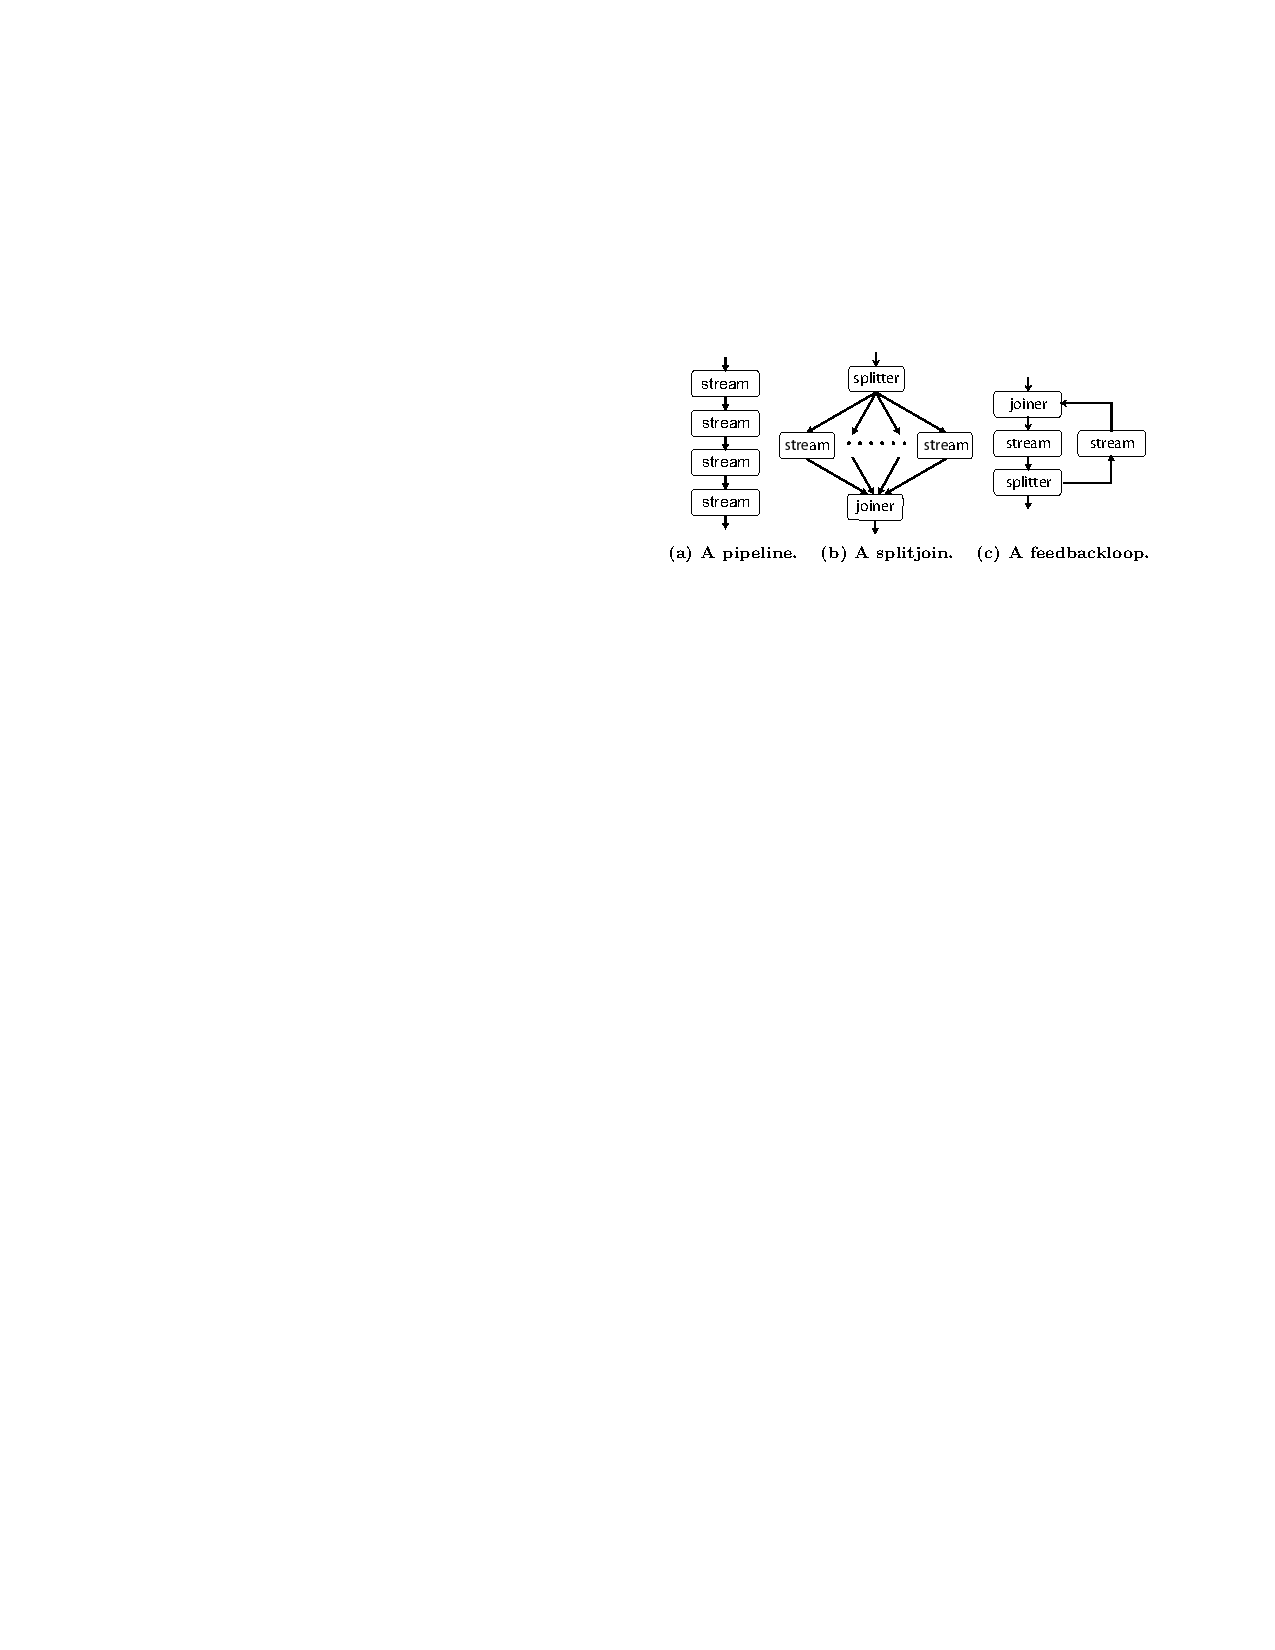
\includegraphics[width=3.3in]{stream-structures.pdf}
%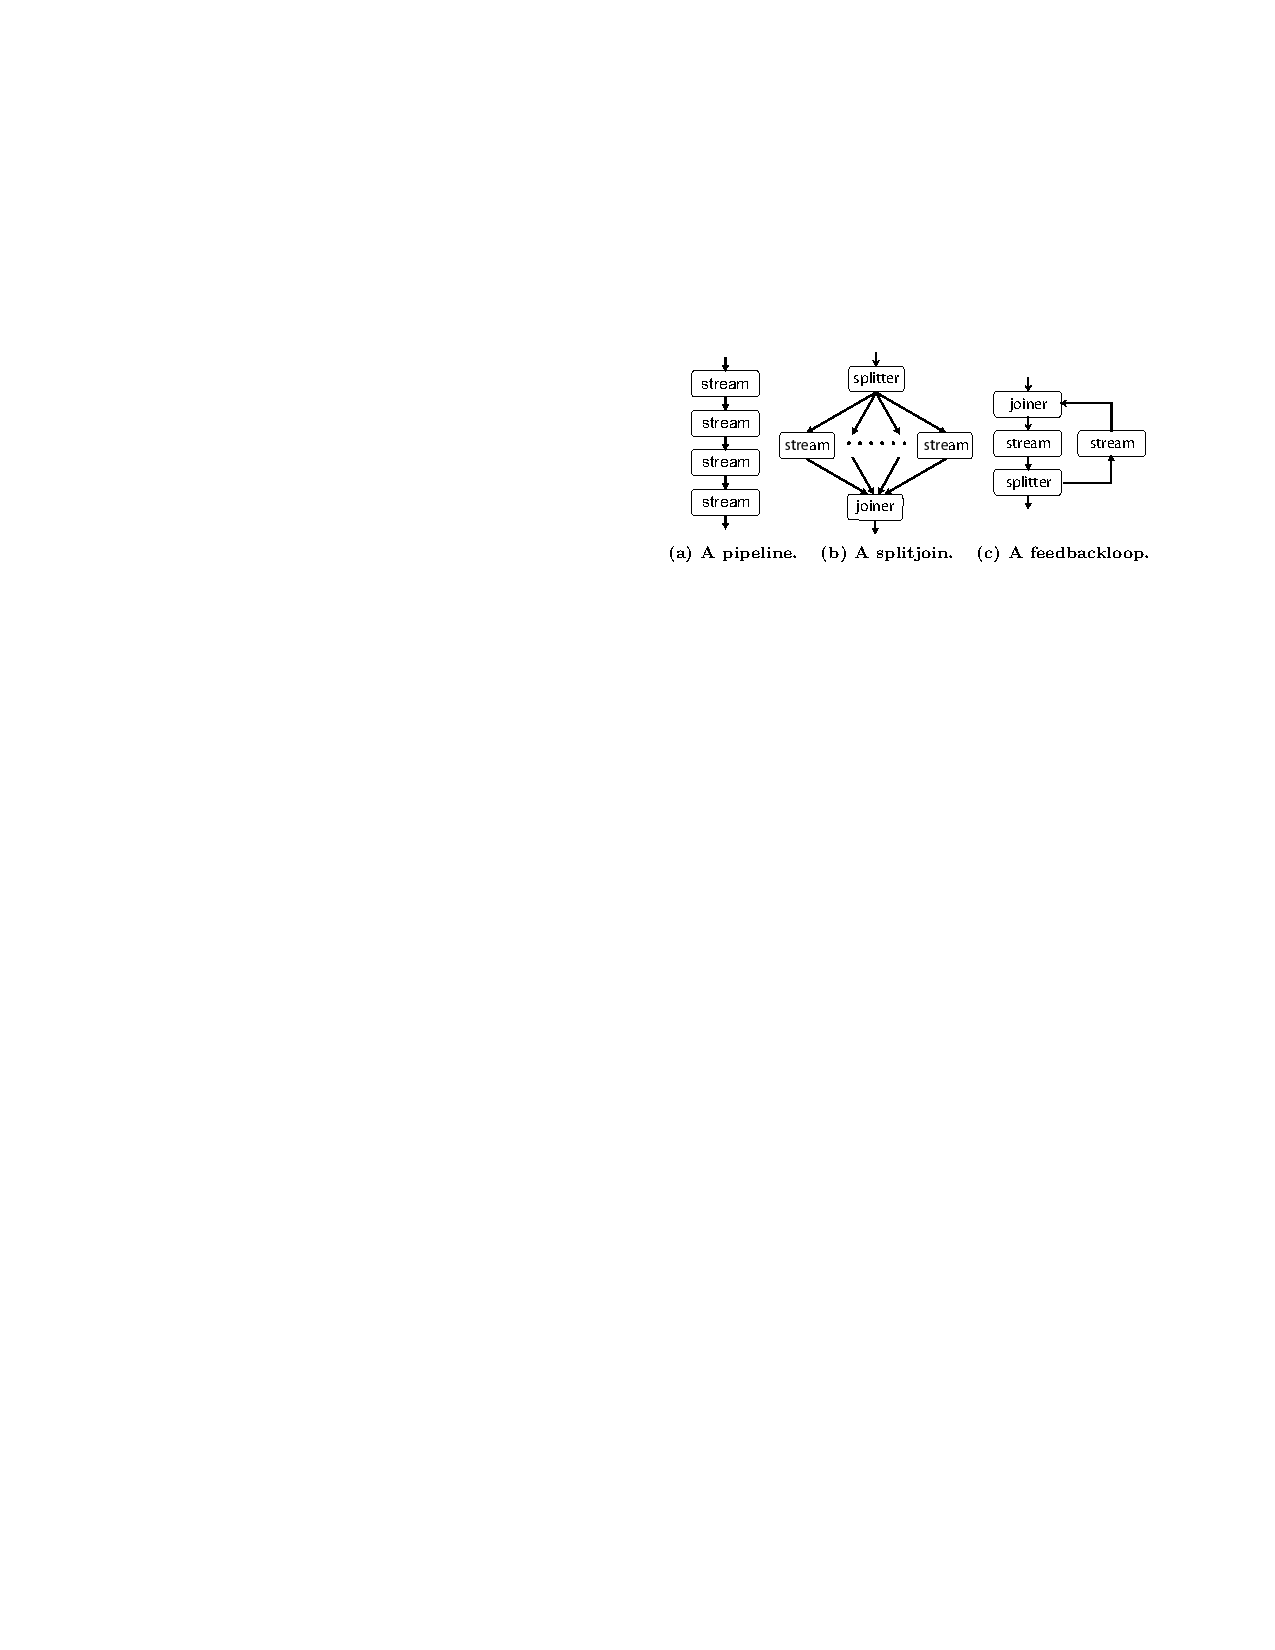
\psfig{file=stream-structures,width=\columnwidth}
\caption{Hierarchical stream structures supported by StreamIt.\protect\label{fig:structures}}
\end{figure}

The StreamIt compiler coarsens the granularity of a stream graph by
applying the {\it fusion} transformation which merges adjacent filters
into a single (large) filter (embedding the schedules of execution in
the merged filter)~\cite{streamit-asplos}.  The {\it fission}
transformation is employed to add data parallelism to a stream graph.
In fission, a single filter without state is duplicated a certain
number of ways and placed in a splitjion construct.  Input items to
the original filter are distributed among the duplicates, termed {\it
  fission products}.  In \S\ref{sec:fission}, we describe how to
extend the fundamental fission transformation to parallelize induction
variable state.

\subsection{The {\StreamIt} Language}
\label{sec:streamit}

The source language for our scheduler is {\StreamIt}: an
architecture-independent programming language for high-performance
streaming applications.  This section contains a very brief overview
of the semantics of {\StreamIt}.  We do not concern ourselves with the
syntax of the language, as it is not relevant to scheduling stream
graphs. A more detailed description of the design and rationale for
{\StreamIt} can be found in~\cite{thies02streamit} or on our
website~\cite{streamitweb}.

\subsubsection{Language Constructs}

The basic unit of computation in {\StreamIt} is the {\filter}. A
{\filter} is a single-input, single-output block with a user-defined
procedure for translating input items to output items.  Every
{\filter} contains a {\work} function, which is comprised of one or
more atomic phases that the filter cycles through during its
steady-state execution. A filter can optionally declare a {\tt
prework} function that executes instead of {\tt work} on the first
invocation of the filter, if special startup behavior is desired.
Filters communicate with their neighbors via FIFO queues, called
{\Channels}, using the intuitive operations of {\tt push(value)}, {\tt
pop()}, and {\tt peek(index)}, where {\tt peek} returns the value at
position {\tt index} without dequeuing the item.  The number of items
that are pushed, popped, and peeked\footnote{{\small We define $peek$
as the total number of items read, including the items popped.  Thus,
we always have that $peek \ge pop$.}} on each invocation are declared
with each phase of the {\work} function.

\begin{figure}
\begin{center}

\begin{minipage}{0.7in}
\centering \psfig{figure=pipeline-buffers.eps,width=0.4049in}
\end{minipage}
~~~~~~
\begin{minipage}{0.8in}
\centering \psfig{figure=splitjoin-steady-state.eps,width=0.6in}
\end{minipage}
~~~~~~
\begin{minipage}{0.8in}
\centering \psfig{figure=feedback-steady-state.eps,width=0.79in}
\end{minipage}

\vspace{0.1in}

{\small ~~~~(a) a pipeline ~~~~~~~ (b) a splitjoin ~~~~ (c) a feedbackloop~~~~}

\caption{\small Sample {\StreamIt} operators.  Each node is labeled
with its peek, pop rates (at top) and push rate (at bottom).  The $L$
{\filter} has been flipped upside-down for clarity.
\label{fig:steady-state}}
\vspace{-18pt}
\end{center}
\end{figure}

%% {\StreamIt}'s representation of a filter is an improvement over
%% general-purpose languages.  In a procedural language, the analog of a
%% filter is a block of statements in a complicated loop nest.  There is
%% no clear abstraction barrier between one filter and another, and
%% high-volume stream processing is muddled with global variables and
%% control flow. The loop nest must be re-arranged if the input or output
%% ratios of a filter changes, and scheduling optimizations further
%% inhibit the readability of the code.

%% In an object-oriented language, one could implement a stream
%% abstraction as a library.  This avoids some of the problems associated
%% with a procedural loop nest, but the programming model is complicated
%% by efficiency concerns--to optimize cache performance, the entire
%% application processes blocks of data that complicate and obscure the
%% underlying algorithm.

%% In contrast to these alternatives, {\StreamIt} places the filter in its
%% own independent unit, making explicit the parallelism and inter-filter
%% communication while hiding the grungy details of scheduling and
%% optimization from the programmer.

{\StreamIt} provides three primitives for composing {\filters} into
hierarchical streams (see Figure~\ref{fig:steady-state}).  The
{\pipeline} construct cascades a set of filters in sequence, with the
output of one connected to the input of the next.  The {\splitjoin}
construct is used to specify independent parallel streams that diverge
from a common {\splitter} and merge into a common {\joiner}---for
example, in the Equalizer of Figure~\ref{fig:radio-ascoded}.  StreamIt
currently supports two types of splitters: duplicate, which broadcasts
its input items to each parallel stream, and round-robin, which
distributes items cyclically to one child after another according to
an array of weights.  The joiner node must be a roundrobin.

The last control construct provides a means for creating cycles in the
stream graph: the {\feedbackloop}. A {\feedbackloop} contains a
{\joiner}, a body operator, a {\splitter}, and a loop operator.  A
{\feedbackloop} has an additional feature to allow it to begin
computation: since there are no data items on the feedback path at
first, the stream needs to enqueue initial values onto the channel.
The number of items pushed onto the feedback path is called the delay,
denoted $delay_{fl}$, for a {\feedbackloop} $fl$.

\subsubsection{Design Rationale}

{\StreamIt} differs from other stream languages in the single-input,
single-output hierarchical structure that it imposes on streams.  This
structure aims to help the programmer by defining clean, composable
modules that admit a linear textual representation.  In addition, it
helps the compiler by restricting certain analyses to a local level
rather than dealing with global properties of the graph.  In the
context of scheduling, hierarchy is also useful because it allows for
the separate compilation of program components.  This enables the
creation of standardized libraries and their distribution in binary
form, rather than source code.  This ability may become important as
streaming languages become more widely used for larger applications.

Another important feature of StreamIt---and one that requires special
support from the scheduler---is the peek construct.  By using the peek
command, a filter can examine an input item at a given index without
removing it from the channel.  This exposes to the compiler the reuse
of input items between successive invocations of a filter's work
function.  A primary example is an FIR filter, which pops 1 item but
peeks N items.  Without the capability to peek, the programmer would
have to maintain a persistent circular buffer within the filter to
retain previous input items.  Apart from being difficult to implement
and understand, this would greatly complicate compiler analysis.  In
particular, the linear analysis and optimization passes within the
StreamIt compiler benefit greatly from analyzing peek statements
directly instead of reverse-engineering internal filter
state~\cite{lamb03}.

\begin{figure}[t]
\begin{center}
\hspace{0.1in} \psfig{figure=radio-ascoded.eps, width=2.8in}
\vspace{-24pt} \caption{\protect\small Block diagram of an FM
Radio. \protect\label{fig:radio-ascoded}}
\vspace{-18pt}
%% \begin{minipage}{0.46in}
%% \centering
%% \psfig{figure=pipeline.eps,width=0.46in} \\
%% \end{minipage}
%% ~
%% \begin{minipage}{1.0in}
%% \centering
%% \psfig{figure=splitjoin.eps,width=0.57in} \\
%% \end{minipage}
%% ~
%% \begin{minipage}{1.02in}
%% \centering
%% \psfig{figure=feedback.eps,width=1.02in} \\
%% \end{minipage}
%% \\ ~ \\ {\bf \protect\small (a) \pipeline ~~~~ (b) \splitjoin ~~~~ (c) \feedbackloop}
%% \caption{\protect\small Stream structures supported by {\StreamIt}.
%% \protect\label{fig:structures}} \vspace{-12pt}
\end{center}
\end{figure}

%% \subsection{Messages}

%% {\StreamIt} provides a dynamic messaging system for passing irregular,
%% low-volume control information between filters and other stream
%% operators.  Messages
%% are sent from within the body of a filter's {\tt work} function,
%% perhaps to change a parameter in another filter.  The central aspect
%% of the messaging system is a sophisticated timing mechanism that
%% allows filters to specify when a message will be received relative to
%% the flow of data items between the sender and the receiver.  With the
%% messaging system, {\StreamIt} is equipped to support full application
%% development--not just high-bandwidth data channels, but also events,
%% control, and re-initialization.

\section{StreamIt Scheduling Concepts}
\label{chpt:sched-basic}

This section introduces the general concepts used for scheduling
{\StreamIt} programs.  Concepts presented here are common with other
systems \cite{ptolemyoverview}.  Section \ref{sec:exec-model} presents
the {\StreamIt} execution model. Section \ref{sec:steady-state}
introduces the concept of a steady state and shows how to calculate
it. Section \ref{sec:init-peeking} explains the need for
initialization of a {\StreamIt} program.
% these languages don't have static scheduling
% \cite{esterel92} \cite{lustre}.

\subsection{{\StreamIt} Execution Model}
\label{sec:exec-model}

A {\StreamIt} program is represented by a hierarchical graph, where
the leaf nodes are filters, splitters, and joiners, and the composite
nodes are pipelines, splitjoins, and feedbackloops.  Edges in the
graph represent data channels, which operate as FIFO queues.

In order for a {\filter} $f$ to execute, it must have at least
$\mt{peek}_f$ items on its input channel.  Execution will decrease the
amount of data on its input channel by $\mt{pop}_f$ and increase the
amount of data on its output channel by $\mt{push}_f$. Similarly, a
{\splitter} $s$ will consume $\mt{pop}_s$ data from its {\Input}
{\Channel} and push $\mt{push}_{s,i}$ data onto its $i$th output
channel, while a joiner $j$ will consume $\mt{pop}_{j,i}$ items from
its $i$th input channel and push $\mt{push}_j$ onto its {\Output}
{\Channel}.

Each filter, splitter, and joiner in the graph has two epochs of
execution: one for initialization, and one for the steady state.
Within each epoch, a given filter can have any number of phases, each
of which is an atomic execution step with its own input and output
rates.  At the start of the program, each node starts in phase $0$ of
the initial epoch.  It then advances through its initialization
phases, executing each a single time before transitioning to phase $0$
of the steady state epoch.  Within the steady state, a filter executes
its steady state phases cyclically.
% (just as in a cyclo-static dataflow graph~\cite{BELP96}).

\subsection{Steady State Schedule}
\label{sec:steady-state}

One of the most important concepts in scheduling streaming
applications is the steady state schedule.  A steady state schedule is
a schedule that the program can repeatedly execute forever.  It has
the property that the amount of data buffered up between any two nodes
does not change from before to after its execution.

A ``steady state'' of a program is a collection of number of times
that every node in the program needs to execute in a steady state
schedule.  It does not impose an order of execution on the nodes in
the program.
\begin{comment}
Not every {\StreamIt} program has a steady state schedule.  It is
possible for a program to have unbalanced production and
consumption of data in {\splitjoins} and {\feedbackloops}. The
amount of data buffered continually increases, and cannot be
reduced, thus making it impossible to create a steady state
schedule for them.  It is also possible that a {\feedbackloop}
does not have enough data buffered up internally in order to
complete execution of a full steady state, and thus deadlocks.
Programs without a valid steady state schedule are not considered
valid {\StreamIt} programs. In other words, all valid {\StreamIt}
programs have a steady state schedule.
\end{comment}

\subsubsection{Minimal Steady State}

We now summarize some of the key properties of steady states, which
are presented in~\cite{lee87static}.  Detailed proofs of these
properties in the context of StreamIt can be found in
\cite{karczma-thesis}.

%% The size of a steady state is defined as the sum of all executions
%% of all the nodes in the program per iteration of the steady state.

%% \begin{definition}
%% A steady state of a stream operator $s$ is represented by vector
%% $m$ of non-negative integers. Each of the elements in $m$
%% represents the number of times a corresponding node in $s$ must be
%% executed in the steady state.
%% \end{definition}

%% Note that $m$ does not impose an order of execution of nodes. Size
%% of a steady state is the total number of executions of all the
%% nodes in the steady state.

The first property concerns the size of a steady state.  The size is
defined to be the sum of the repetitions of all nodes in the schedule.

\begin{theorem}[Minimal Steady State Uniqueness]
A {\StreamIt} program that has a valid steady state, has a unique
minimal steady state.
\end{theorem}

This means that for every valid {\StreamIt} program, there is a unique
set of steady state multiplicities that fires as few nodes as
possible.  Our scheduler will produce schedules that execute exactly
the minimal steady state of a program.

\begin{comment}
\begin{proof}[Minimal Steady State Uniqueness]
Assume that there are two different minimal steady states with
same size.  Let $m$ and $q$ denote vectors representing the two
steady states. Let $\sum_i m_i$ denote size of schedule $m$ and
$\sum_i q_i$ denote size of schedule $q$. Note that since both $m$
and $q$ are minimal steady states, $\sum_i m_i = \sum_i q_i$.
Since the schedules are different, there must be some $j$ for
which $m_j \ne q_j$. Assume without loss of generality that $m_j <
q_j$. Since a steady state does not change the amount of data
buffered between nodes, the node producing data for node $i$ must
also execute less times than corresponding node in $q$. Similarly,
the node consuming data produced by node $j$ also must execute
less times than the corresponding node in schedule $q$. Since a
{\StreamIt} program describes a connected graph, it follows that
$\forall i, m_i < q_i$.  Thus $\sum_i m_i \ne \sum_i q_i$, which
is a contradiction. Thus there cannot be two different minimal
steady state.
\end{proof}

\begin{corollary}[Minimal Steady State Uniqueness]
\label{corollary:minimal-state}
The additional property we have from the above proof is that if
$m$ represents a minimal steady and $q$ any other steady state,
then $\forall i, m_i < q_i$.
\end{corollary}

\begin{lemma}[Composition of Steady Schedules]
\label{lemma:composition}
If $m$ and $q$ are two steady states for a {\StreamIt} program, then
$m + q$ is also a steady state.
\end{lemma}

The above lemma is true because neither $m$ nor $q$ change the
amount of data buffered in the {\Channels}.  Thus a composition of
the steady states does not change the amount of data buffered in
the {\Channels}, which makes the composition also a steady schedule.

\begin{corollary}[Composition of Steady Schedules]
\label{corollary:composition}
If $m$ and $q$ are two steady states, and $\forall i, m_i > q_i$,
then $w = m - q$ is also a steady state.
\end{corollary}

If $q$ is a steady state and $m = w + q$ is a steady state, then
$w$ must not change the amount of data buffered in {\Channels}. Thus
$w$ must be a steady state.
\end{comment}

\begin{theorem}[Multiplicity of Steady States] If a
{\StreamIt} program has a valid steady state, then all its steady
states are strict multiples of its minimal steady state.
\label{thm:multiplicity}
\end{theorem}

\begin{comment}
\begin{proof}[Multiplicity of Minimal Steady State]
Assume that there exists a steady state that is not a multiple of
the minimal steady state.  Let $m$ denote the minimal steady
state. Let $q$ denote the other steady state.  Note that $w = q -
m$ is still a steady state, as long as all elements of $w$ remain
non-negative (by Corollary \ref{corollary:composition}).  Repeat
subtracting $m$ from $q$ until no more subtractions can be
performed without generating at least one negative element in
vector $w$.  Since $q$ is not a multiple of $m$, $w \ne 0$. But
since we cannot subtract $m$ from $w$ any further, $\exists i, m_i
> w_i$.  Since $m$ is a minimal steady state and $w$ is a steady
state, this is impossible due to Corollary
\ref{corollary:minimal-state}. Thus there are no steady states
that are not multiples of the minimal steady schedule.
\end{proof}
\end{comment}

This property means that in order to find a minimal steady state
schedule of a stream operator, we can find any of its steady states
and divide it by the $gcd$ of executions of all its children to find
the minimal steady state schedule.

\subsubsection{Calculating Minimal Steady States}
\label{sec:calc-min-steady}

For a general stream graph, the minimal steady state can be calculated
in a linear algebra framework by formulating a set of balance
equations~\cite{lee87static}.  However, with StreamIt we leverage the
structure of the stream graph to calculate steady states in a
hierarchical manner.  That is, a minimal steady state is calculated
for all child operators of a {\pipeline}, {\splitjoin} and
{\feedbackloop}, and then the schedule is computed for the actual
parent operator using these minimal states as atomic executions.  This
approach is useful in the context of separate compilation, where the
entire graph might not be available at compile time; additionally, the
steady state multiplicity of a given node in relation to its parent is
useful for our scheduling algorithms.

For brevity, we omit the equations for finding the minimal steady
states.  The steady states are calculated hierarchically; filters with
multiple phases are represented by a single, coarser phase for the
sake of the steady-state schedule.  Details can be found
in~\cite{karczma-thesis}.  For example, the minimal steady states of
the stream graphs in Figure~\ref{fig:steady-state} are as follows:

\mbox{}
~ \vspace{-20pt} \\
\begin{equation*}
\begin{tabular}{ll}
\mbox{Sample Pipeline}: & \mt{steady}(A) = 4 \\
~ & \mt{steady}(B) = 6 \\
~ & \mt{steady}(C) = 9 \\
~ & \mt{steady}(D) = 3 \\
~ & ~ \vspace{-4pt} \\
\mbox{Sample SplitJoin}: & \mt{steady}(splitter) = 2 \\
~ & \mt{steady}(A) = 2 \\
~ & \mt{steady}(B) = 1 \\
~ & \mt{steady}(joiner) = 2 \\
~ & ~ \vspace{-4pt} \\ 
\mbox{Sample FeedbackLoop}: & \mt{steady}(joiner) = 6 \\
~ & \mt{steady}(B) = 15 \\
~ & \mt{steady}(splitter) = 5 \\
~ & \mt{steady}(L) = 3 \vspace{4pt}\\
\end{tabular}
\end{equation*}
Note that these numbers represent the multiplicity of each node in one
steady state execution of its parent.  In Section~\ref{chpt:phased},
we consider how to order these executions to form a valid schedule.

%% Executing a full steady state of an operator is referred to as
%% ``executing an operator". The notation for $peek$, $pop$ and $push$ is
%% is extended to mean entire operators in their minimal steady state
%% execution.  That is, a {\pipeline} $p$ will consume $o_p$ data,
%% produce $u_p$ data and peek $e_p$ data on every execution of its
%% steady state.  Again, in the hierarchical view of {\StreamIt}
%% programs, a child operator of a {\pipeline} will execute its steady
%% state atomically.

%% A steady state of a stream operator $s$ is represented by an
%% ordered set $S_s$ of elements, $S_s = \{m, N, c, v\}$. The set
%% includes a vector $m$, which describes how many times each
%% {\StreamIt} node of the operator will be executed in the steady
%% state, a corresponding ordered set $N$ which stores all the nodes
%% of the operator, a vector $c$, which holds values $[e_s, o_s,
%% u_s]$ for stream operator $s$, and a vector $v$ which holds number
%% of steady state executions of all direct children of $s$. $m$ and
%% $v$ are not the same vector, because $m$ refers to nodes in the
%% subgraph, while $v$ refers only to the direct children, which may
%% be {\filters}, {\pipelines}, {\splitters} and {\feedbackloops}.
%% For a stream operator $s$, set $S$ is denoted as $S_s$ and the
%% elements of $S_s$ are denoted as $S_{s,m}$, $S_{s,N}$, $S_{s,c}$
%% and $S_{s,v}$.

%% Note, that a steady state does not say anything about the ordering
%% of the execution of nodes, only how many times each node needs to
%% be executed to preserve amount of data buffered by the operator.

%% We omit the equations for calculating the minimal steady states
%% for brevity. Details can be found in Appendix \ref{apx:eqs}. As an
%% example, the {\splitjoin} from Figure \ref{fig:steady-state}(b) has
%% the following steady state:

%% \begin{displaymath}
%% S_{sj} = \left\{
%% \begin{array}{c}
%% 2 * S_{sj_0, m} \circ 1 * S_{sj_1, m} \circ [2\ 2], \\
%% S_{sj_0, N} \circ S_{sj_1, N} \circ \{sj_s, sj_j\}, \\
%% \left[
%% \begin{array}{c}
%% 2 * 3 \\ 2 * 3 \\ 2 * 4
%% \end{array}
%% \right], \left[
%% \begin{array}{c}
%% 2 \\ 1 \\ 2 \\ 2
%% \end{array}\right]
%% \end{array} \right\}
%% \end{displaymath}

\subsection{Initialization Schedule}
\label{sec:init-peeking}

Unlike traditional SDF graphs, StreamIt programs may require a
separate schedule for initialization.  This is for two reasons.
First, each filter might contain an initialization stage, where the
input and output rates are different than in the steady state.  But
even without the initialization epoch, an initialization schedule is
necessary if any filter makes use of StreamIt's $peek$ construct, in
which input items can be examined without being consumed.

To understand the impact of peeking on scheduling, consider a filter
$f$, with $\mt{peek}_f = 2$ and a $\mt{pop}_f = 1$. When a {\StreamIt}
program is first run, there is no data present on any of the
{\Channels} (ignoring the case of a feedbackloop delay).  This means
that for the first execution, {\filter} $f$ requires that two data
items be pushed onto its {\Input} {\Channel}.  After the first
execution of $f$, it will have consumed one data item, and left at
least one data item on its {\Input} {\Channel}.  Thus in order to
execute $f$ for the second time, no more than one extra data item
needs to be pushed onto $f$'s {\Input} {\Channel}.  The same situation
persists for all subsequent executions of $f$ -- no more than one
additional data item is required on $f$'s {\Input} {\Channel} in order
to execute $f$.

This example illustrates that the first execution of a {\filter} may
require special treatment.  Namely, some nodes will need to push extra
items at the start of execution so that downstream filters can fire
for the first time.  Due to this condition, a {\StreamIt} node may
need to be initialized before it can enter steady state execution.

%% \subsection{Schedules}
%% \label{sec:general:schedules}

%% Once a program has been initialized, it is ready to execute its
%% steady state. In order to do this, a steady state schedule needs
%% to be computed. The steady states computed above do not indicate
%% the ordering of execution of the nodes, only how many times the
%% nodes need to be executed.

%% A schedule is an ordering of nodes in a {\StreamIt} operator. In
%% order to execute the schedule, we iterate through all of its nodes
%% in order of appearance and execute them one by one.  For example
%% in order to execute schedule $\{ABBCCBBBCC\}$ we would execute
%% node A once, node B twice, node C two times, node B three times
%% and node C twice again, in that order. In order to shorten the
%% above schedule we can run-length encode it.  The schedule becomes
%% $\{A \{2B\}\{2C\}\{3B\}\{2C\}\}$.

\section{Phased Scheduling}
\label{chpt:phased}

A schedule for a given hierarchical node of a {\StreamIt} program is a
list of the node's immediate children, specifying the order in which
they should be executed.  More precisely, since filters (and, as we
will see, hierarchical nodes as well) can have multiple phases, a
schedule is a list of phases of child nodes.  In order for a schedule
to be legal, it must satisfy two conditions: first, for every
execution of a node, a sufficient amount of data must be present on
its {\Input} {\Channel}(s); second, in the case of the steady state,
an infinite repetition of the schedule must require a finite amount of
memory.  The second condition is ensured by using the steady state
multiplicities calculated in the previous section, while the first
condition is one that we must respect when choosing an ordering for
the nodes.

Our phased scheduling algorithm, shown in Figure~\ref{fig:phasealg},
operates in a hierarchical fashion.  That is, it constructs a schedule
for a given pipeline, splitjoin, or feedbackloop as a sequence of the
schedules of its children.  A schedule is represented as a sequence of
phases.  In the base case of a filter, these phases are specified by
the StreamIt program (with one small modification, described below),
while at hierarchical nodes they are computed by our algorithm.  To
schedule an entire StreamIt program, our algorithm should be applied
as a post-order traversal of the stream graph.

Intuitively, our algorithm is based on the observation that a
hierarchical stream displays cyclic behavior as it executes its
components.  At the coarsest level of granularity, these cycles are
evident in the steady state schedule: each iteration of the steady
state is exactly the same.  The aim of our algorithm is to exploit a
finer level of granularity in execution behavior---the basic unit
being a phase of the push schedule for the stream.  Generally
speaking, a phase of the push schedule holds the smallest sequence of
filter executions that will both consume input and produce output for
the stream.  Our algorithm allows a parameterized level of granularity
by collapsing some of these fine-grained phases together and shuffling
the resulting schedule so that the phases of a given child stream are
all adjacent.  As we demonstrate below, a single appearance schedule
and minimum latency schedule are both special cases of a parameterized
phased schedule.  For a more mathematical description of the phased
scheduling technique, see~\cite{karczma-thesis}.

\subsection{Algorithm Details}

We now consider in more detail the pseudocode in
Figure~\ref{fig:phasealg}; refer to Figures~\ref{fig:sjex}
and~\ref{fig:sjexlabel} for an example.  The algorithm inputs a Stream
{\tt s} and returns a sequences of phases that represent the schedule
for that stream.  It also inputs two additional parameters: {\tt
maxPhases}, which specifies the maximum number of phases in the
resulting schedule, and {\tt mode}, which indicates whether we are
scheduling for the initial or steady-state epoch.  The algorithm
starts by assembling a series of fine-grained phases, each of which
corresponds to a push schedule as built by the {\tt pushSchedule}
routine.

The {\tt pushSchedule} routine simulates a push schedule until the
bottom node is fired at least once (in most cases, this will
correspond to an output being produced).  A push schedule is one in
which downstream nodes are fired as much as possible before upstream
nodes are considered.  The routine starts with the entrance node of
the stream, {\it i.e.,} the first child of a pipeline, the splitter of
a splitjoin, or the joiner of a feedbackloop.  It then pushes live
items as far forward as possible, only executing the entrance node
again if the exit node could not fire.

\begin{figure}[t]
\vspace{3pt}
\psfig{figure=pseudocode5.eps,width=3.5in}
\vspace{-26pt}
\caption{\small Phased Scheduling Algorithm.\protect\label{fig:phasealg}}
\vspace{-8pt}
\end{figure}

There are two subtleties in the {\tt pushSchedule} procedure.  First,
note that it always flushes extra items from the stream: the exit node
might fire multiple times, even though all firings were caused by a
single execution of the entrance node.  Second, in the case of a
feedbackloop, it is careful to push items around the feedback path
even after the splitter (the exit node) has fired.  That is, the
ranking of nodes in a feedback loop is $(\mt{joiner}, \mt{body},
\mt{splitter}, \mt{loop})$, and pushing of items through the loop node
is necessary to ensure a correct steady-state schedule.

The {\tt phasedSchedule} routine builds up a maximal list of phases
from the push schedule.  In the steady state, this list is complete
when each node has completed its steady state repetitions, while in
the initialization mode, simulation is finished when each node has
executed its initial phases.  To ensure that the initialization
schedule provides enough data items for the peeking requirements of
the steady state, we add an extra initialization phase to each filter
before running the algorithm.  For filter $f$, this phase has rates
$\mt{peek'}=\mt{peek}_f - \mt{pop}_f, \mt{pop'}=\mt{push'}=0$.  Since
this phase must execute in the initial schedule, it ensures that there
will be $\mt{peek}-\mt{pop}$ items present at the start of the steady
state.  A steady state schedule is then possible to construct, since
the filter can return the buffer to this state by firing once with
$\mt{peek}$ items on the channel.

Once it has gathered the list of maximally fine-grained phases, the
{\tt phasedSchedule} algorithm makes two modifications.  First, it
combines some adjacent phases so that only {\tt maxPhases} are
returned.  Combination works simply by concatenating the sequence of
child executions from the given phases.  Second, even if no phases are
combined, the algorithm re-arranges the order of child phases so that
all phases corresponding to a given stream are adjacent.  This is an
attempt to provide a canonical form for a given series of executions,
so that phases with the same form can be compressed in the resulting
schedule~(see Section~\ref{sec:schedrep}).

\begin{figure*}[t]
\psfig{figure=splitjoin-sample-tiny2.eps,width=7in}
\caption{{\small Example construction of phased schedules for the
splitjoin of Figure~\ref{fig:sjexlabel}.  First, execution is
simulated for one steady state according to a push schedule; the
stream graph is labeled with the number of items on each channel
following the firing of a shaded node.  Then, fine-grained phases are
formed that include executions of both the entry (A) and exit (D)
nodes.  Finally, the fine-grained phases are combined into
$\mt{maxPhases}$ phases, each of which is factored into a single
appearance schedule.  Note that buffer size increases with the
granularity of the phases, as shown at right.\protect\label{fig:sjex}}}
\vspace{-12pt}
\end{figure*}

\begin{figure}
\vspace{6pt}
\begin{minipage}{1.3in}
\begin{center}
\psfig{figure=splitjoin-sample2.eps,width=0.8in} 
\end{center}
\end{minipage}
\begin{minipage}{1.75in}
\caption{\small Example splitjoin to illustrate phased scheduling.
Each node is annotated with its input and output
rates.\protect\label{fig:sjexlabel}}
\end{minipage}
\vspace{-6pt}
\end{figure}


Note that the pseudocode given in Figure~\ref{fig:phasealg} specifies only
the behavior of the algorithm, rather than the implementation.  In our
implementation, we avoid symbolic execution of the entire steady state
by calculating, from the bottom-up, the number of node firings that
will be required in each phase.  If upstream nodes produce more data
than is necessary, then we drain this data through the stream by
firing downstream nodes again.  In this technique, each child is
visited no more than twice per calculation of a parent phase.

%% \begin{table*}[t] \centering  \scriptsize
%% \begin{tabular}{|c|c|c|c|c|c|c|c|c|c|c|c|}
%% \hline
%% \multicolumn{4}{|c|}{data in {\Channel}} & \multicolumn{4}{c|}{\parbox{1in}{\centering phase executions left}} & \parbox{0.5in}{\centering child considered} & \parbox{0.6in}{\centering phases executed} & \parbox{0.6in}{\centering {\pipeline} consumption} \\
%% \cline{1-8} $in_A$ & $out_A$ & $in_B$ & $out_B$ & split & A & B & join & & & \\
%% \hline 0 (0) & 0 (0) & 0 (0) & 0 (0) & 0 & 0 & 1 & 0 & join & - & $[0\ 0\ 0]$ \\
%% \hline 0 (0) & 0 (0) & 0 (0) & 0 (0) & 0 & 0 & 1 & 0 & A & - & $[0\ 0\ 0]$ \\
%% \hline 0 (0) & 0 (0) & 0 (0) & 0 (0) & 0 & 0 & 1 & 0 & B & $A^i_{B,0}$ & $[0\ 0\ 0]$ \\
%% \hline 0 (0) & 0 (0) & 0 (1) & 0 (0) & 0 & 0 & 0 & 0 & split & split & $[3\ 3\ 0]$ \\
%% \hline 2 (0) & 0 (0) & 1 (0) & 0 (0) & 0 & 0 & 0 & 0 & A & $A^i_{A,0}$ & $[0\ 0\ 0]$ \\
%% \hline 0 (0) & 1 (0) & 1 (0) & 0 (0) & 0 & 0 & 0 & 0 & B & - & $[0\ 0\ 0]$ \\
%% \hline 0 (0) & 1 (0) & 1 (0) & 0 (0) & 0 & 0 & 0 & 0 & join & - & $[0\ 0\ 0]$ \\
%% \hline 0 (0) &  1 (0) &  1 (0) &  0 (0) & \multicolumn{7}{|c|}{init phase 0 done, init done} \\
%% \hline 0 (0) & 1 (0) & 1 (0) & 0 (0) & 2 & 2 & 1 & 2 & join & join & $[0\ 0\ 4]$ \\
%% \hline 0 (0) & 0 (0) & 1 (0) & -3 (3) & 2 & 2 & 1 & 2 & A & - & $[0\ 0\ 0]$ \\
%% \hline 0 (0) & 0 (0) & 1 (0) & -3 (3) & 2 & 2 & 1 & 1 & B & $A_{B,0}$ & $[0\ 0\ 0]$ \\
%% \hline 0 (0) & 0 (0) & -1 (2) & 3 (0) & 2 & 2 & 0 & 2 & split & $\{2split\}$ & $[6\ 6\ 0]$ \\
%% \hline 4 (0) & 0 (0) & 1 (0) & 3 (0) & 0 & 2 & 0 & 2 & A & $\{2A_{A,0}\}$ & $[0\ 0\ 0]$ \\
%% \hline 0 (0) & 2 (0) & 1 (0) & 3 (0) & 0 & 0 & 0 & 0 & B & - & $[0\ 0\ 0]$ \\
%% \hline 0 (0) & 2 (0) & 1 (0) & 3 (0) & 0 & 0 & 0 & 1 & join & join  & $[0\ 0\ 4]$ \\
%% \hline 0 (0) &  1 (0) &  1 (0) &  0 (0) & \multicolumn{7}{|c|}{phase 0 done, steady state schedule done} \\
%% \hline
%% \end{tabular}
%% \caption[Execution of Minimal Latency Scheduling Algorithm on a
%% {\splitjoin}]{Execution of Minimal Latency Scheduling Algorithm on
%% {\splitjoin} from Figure \ref{fig:steady-state}(b). In the ``data
%% in {\Channel}'' columns, the first value represents the actual
%% number of data in the {\Channel}, which can be negative due to
%% data borrowing. The second value is the minimal number of data
%% items borrowed from the {\Channel}.}
%% \label{tbl:min-lat-sj}
%% \end{table*}

%% Table \ref{tbl:min-lat-sj} contains a trace of execution of our
%% algorithm on the sample {\splitjoin} from Figure
%% \ref{fig:steady-state}(b). Below is the phased schedule for the
%% {\splitjoin}. Note that this example produces a phased single
%% appearance schedule.

%% \begin{displaymath} \scriptsize
%% P_{sj} = \left\{
%% \begin{array}{c}
%% T_{sj} = \left\{
%% \begin{array}{c}
%% A_{sj,0} = \left\{ \{\{2 split\}\{2A\}B\{2 join\}\}, \left[\begin{array}{c} 6 \\ 6 \\ 8 \end{array}\right]\right\} \\
%% \end{array}\right\}, \\
%% I_{sj} = \left\{ A^i_{sj,0} = \left\{
%% \{split\ A^i_{A,0}\ A^i_{B,0}\}, \left[\begin{array}{c} 3 \\ 3 \\ 0 \\
%% \end{array}\right]\right\}
%% \right\}, \\
%% c_{sj} = \left[ \begin{array}{c} 6 \\ 6 \\ 8 \end{array} \right],
%% c^i_{sj} = \left[ \begin{array}{c} 3 \\ 3 \\ 0 \end{array}
%% \right],
%% \end{array}
%% \right\}
%% \end{displaymath}

\subsection{Generalizing Other Techniques}

As alluded to above, single appearance scheduling and minimum latency
scheduling are special cases of our parameterized phased scheduling
algorithm.  A single appearance schedule is defined as a schedule
where each node appears in one position of the loop nest denoting the
schedule.  Because the nodes within a phase are sorted by child
stream, this is equivalent to a phased schedule with a single phase:
\[
\small
\begin{array}{rcl}
\mt{singleAppSchedule}[s]  & = & \langle \mt{phasedSchedule}(s, 1, \mbox{INIT}), \\
                         ~ & ~ & ~ \mt{phasedSchedule}(s, 1, \mbox{STEADY}) \rangle
\end{array}
\]

A minimum latency schedule exhibits the following property: if $i$
input items have been consumed by a hierarchical node when it produces
its $j$th output item, then there does not exist a schedule which
produces $j$ output items while consuming less than $i$ input items.
This condition is necessary and sufficient for a schedule to be
minimum latency.  We can construct a minimum latency schedule as a
phased schedule with an unlimited number of phases:
\[
\small
\begin{array}{rcl}
\mt{minLatencySchedule}[s] & = & \langle \mt{phasedSchedule}(s, \infty, \mbox{INIT}), \\
                         ~ & ~ & ~ \mt{phasedSchedule}(s, \infty, \mbox{STEADY}) \rangle
\end{array}
\]
This schedule is guaranteed to be minimum latency, since it is
comprised of push phases that do not fire the entrance node once the
exit node has been fired (see {\tt pushSchedule} in
Figure~\ref{fig:phasealg}).

Thus, single appearance and minimum latency schedules represent
extreme values of the {\tt maxPhases} parameter.  Other values of {\tt
maxPhases} indicate compromises between these two extremes.  Also,
note that different levels of granularity could be applied to
different streams in the same graph, depending on the constraints; the
algorithm does not depend on the granularity of the children when it
is scheduling a parent node.

\subsection{Scheduling Feedback Loops}

Some feedback loops require a minimum number of phases in order to
construct a valid schedule.  This is because if the latency of child
streams is too high, then a node could deadlock waiting for its own
(upcoming) output to propagate through the loop.  For example, in our
GSM benchmark, there is a tightly constrained feedback loop (see
Figure~\ref{fig:gsm}).  While it is impossible to schedule this loop
with a single appearance schedule, a minimum latency schedule results
in a legal ordering (see~Figure~\ref{fig:gsm-phases}).

Figure~\ref{fig:feedalg} provides an algorithm for calculating the
minimum number of phases that are required to schedule a feedback
loop.  The routine's functionality is similar to the phased scheduler,
except for one key difference: the joiner is executed as much as
possible before the items that it pushes are propagated around the
loop.  This ensures that the reshuffling step of the phased scheduling
algorithm will be legal, since no element in the schedule will depend
on items that it produced earlier in the same phase.  Note that the
{\tt phasedSchedule} algorithm gives an undefined result if a given
loop is impossible to schedule with the requested number of phases;
thus, {\tt phasesForFeedback} should always be called first to see how
many phases are needed.

\begin{figure*}[t]
\centering
\psfig{figure=gsmfl-sched.eps,width=5.2in}
\vspace{-4pt}
\caption{\small Phased minimum latency schedule for one steady state
execution of the feedback loop of Figure~\ref{fig:gsm}.  Nodes are
labeled with the number of times they fire in a given phase.  No
single appearance schedule exists for this
loop.\protect\label{fig:gsm-phases}}
\vspace{-3pt}
\end{figure*}

\begin{figure}
\begin{center}
\vspace{-6pt}
\psfig{figure=gsmfl.eps,width=2in}
\vspace{-6pt}
\caption{\small A tightly coupled feedback loop that appears as one component
of our GSM benchmark.  Nodes are labeled with their pop and push
rates.  \protect\label{fig:gsm}}
\end{center}
\vspace{-12pt}
\end{figure}

\subsection{Schedule Representation}
\label{sec:schedrep}

In the discussion above, a schedule is represented simply as a
sequence of phases for child nodes.  However, since this
representation can become large for some programs, our implementation
employs compression to keep code size to a minimum.  

We compress the schedule in three simple ways.  First, we collect
repetitions of identical phases into a loop.  For example, if {\tt A}
is a phase:
\[
\mbox{{\tt A=BBB}} ~\rightarrow~ \mbox{{\tt A=\{3B\}}}
\]
Second, if a hierarchical phase contains only one execution of a
child, we substitute all occurrences of the parent with a direct call
to the child:
\[
\mbox{{\tt A=BCD, C=E}} ~\rightarrow~ \mbox{{\tt A=BED}}
\]
Finally, if a phase is used only once, then it can be replaced by its
child phases, even if there are multiple children:
\[
\mbox{{\tt A=BCD, C=EFG, C}}~\mt{used}~\mt{only}~\mt{once}~ ~\rightarrow~ \mbox{{\tt A=BEFGD}}
\]
To improve the compression of the schedule, we repeatedly apply the
above three transformations until no further changes can be made.

%% During testing it was found that in some applications some operators
%% had many phases that were identical to other phases of the
%% operator. Instead of including these phases in the final schedule
%% multiple times, they were listed only once, and references to the
%% duplicate phases have been replaced with references to the one copy.

%% This optimization lead to improvements in schedule size for two
%% reasons. First, operators now have fewer phases, so their schedules
%% take up less space. Second, applications using the phased schedules
%% can now execute the same phase multiple times in a row, which was
%% optimized out using run length encoding.

In the future, an additional optimization could be explored regarding
schedule compression.  Instead of representing different phases for a
given stream by distinct entries in the schedule, we could record only
the name of the stream in the schedule and postpone the resolution of
the current phase number until runtime.  This would allow more
opportunities for schedule compression, as two different phases would
be considered equal if they call the same child streams, rather than
requiring them to call the same phases on those children.  However,
proper evaluation of this technique would need to take into account
the overhead of this indirection at runtime, and we do not evaluate it
here.

\begin{figure}
\psfig{figure=pseudocode6.eps,width=3.5in}
\vspace{-16pt}
\caption{\small Algorithm to detect the minimum number of phases required by
a given feedback loop.\protect\label{fig:feedalg}}
\end{figure}

%\section{Pseudo Single Appearance Hierarchical Scheduling}
\label{chpt:hierarchical}

In this section we present Pseudo Single Appearance Hierarchical
Scheduling, a technique which is quite effective for scheduling
{\StreamIt} programs, but which cannot schedule all programs, and
which may require the buffers to be very large.

\begin{comment}
Section \ref{sec:hierarchical:motivation} provides some motivation
for hierarchical scheduling.
\end{comment}
Section \ref{sec:hierarchical-notation} presents the notation used
for hierarchical schedules. Section \ref{sec:sas} provides an
algorithm for computing pseudo single appearance hierarchical
schedules.

\begin{comment}
\subsection{Motivation}
\label{sec:hierarchical:motivation}

As has been explained in Section \ref{sec:sched-vs-buffer}, the
ordering of execution of nodes in a {\StreamIt} program can have a
significant effect on the amount of resources necessary to execute
the schedule.  The two important factors to consider when creating
the schedule is amount of buffering necessary to execute the
schedule, and the amount of space necessary to store the schedule.
The amount of buffering necessary is controlled by the ordering of
execution of nodes of the {\StreamIt} graph.  The amount of storage
necessary to store the schedule is controlled by the encoding of
the schedule.  As a general rule, ordering which minimizes the
buffering space requirements is fairly irregular and difficult to
encode efficiently.

\begin{figure}
\centering \psfig{figure=hierarchical-sample.eps,width=1in}
\caption[Stream operator for hierarchical scheduling]{A sample
stream operator used for hierarchical scheduling.}
\label{fig:sample-sj}
\end{figure}

One technique used for encoding schedules is to form loop-nests of
sub-schedules and repeat them multiple times, until a steady-state
schedule is reached.  For example, the operator in Figure
\ref{fig:sample-sj} has a following steady state:

\begin{displaymath}
S_{s} = \left\{ \left[
\begin{array}{c}
9 \\ 6 \\ 18 \\ 18 \\ 4 \\ 4
\end{array} \right], \left[
\begin{array}{c}
A \\ C \\ D \\ split \\ join \\ B
\end{array}
\right], \left[
\begin{array}{c}
54 \\ 54 \\ 40
\end{array}
\right], \left[
\begin{array}{c}
9 \\ 2 \\ 4
\end{array}
\right]\right\}
\end{displaymath}

\noindent Thus one steady state schedule for this operator can be
$$\{9\{A\{2 split\}\{2D\}\}\}\{2\{\{3C\}\{2 split\}\{2B\}\}\}$$
Here, $\{A\{2 split\}\{2D\}\}$ and $\{\{3C\}\{2 split\}\{2B\}\}$
are the inner nests, executed 9 and 2 times respectively.

If, the overall schedule has every {\StreamIt} node appear only
once (as in the example above), the technique is called Single
Appearance Scheduling \cite{bhattacharyya94looped}. One of
difficulties in using Single Appearance Scheduling is finding a
good way to form loop-nests for the sub-schedules, because the
buffering requirements can grow quite large.  An example of this
has been presented in Section \ref{sec:sched-vs-buffer}.

{\StreamIt} provides the scheduler with a pre-existing
hierarchical structure. While it is possible to use techniques
developed for Single Appearance Scheduling to create valid
schedules for {\StreamIt} programs, Single Appearance Scheduling
does not satisfy all requirements of an effective {\StreamIt}
scheduler. This is because some {\feedbackloops} cannot be
scheduled using Single Appearance Scheduling techniques. This
difficulty arises because the amount of data provided to the
{\feedbackloop} by the $delay_{fl}$ variable is not sufficient to
perform a complete steady-state execution of the loop, thus
preventing the schedule for the {\feedbackloop} to be encoded with
only a single appearance of every node in the schedule.

The solution to this problem is to have the same node appear
multiple times in the schedule.  While this solves the problem of
inability to schedule some {\feedbackloops}, it introduces another
problem: which nodes should appear several times, and how many
times should they be executed on each appearance.  The solution
proposed here goes half-way to solve the problem. A more effective
solution will be proposed in Chapter \ref{chpt:phased}.

In hierarchical scheduling we use the pre-existing structure
(hierarchy) to determine the nodes that belong in every loop-nest.
Basically, every operator receives its own loop-nest, and treats
steady-state execution of its children as atomic (even if those
children are operators whose executions can be broken down into
more fine-grained steps). In the example above, the {\pipeline}
has a {\splitjoin} child.  The {\splitjoin} is responsible for
scheduling its children (nodes $C$, $B$, $split$ and $join$).  The
{\pipeline} will use the {\splitjoin}'s schedule to create its own
steady state schedule. Here the {\splitjoin}'s schedule can be
$T_{sj} = \{\{9 split\}\{3C\}\{9D\}\{2 join\}\}$, thus making the
{\pipeline}'s schedule \footnote{Notation for this schedule is
explained in next section (Section
\ref{sec:hierarchical-notation}).} $$T_{pipe} = \{\{9A\}\{2
T_{sj}\}\{4B\}\} = \{\{9A\}\{2\{\{9 split\}\{3C\}\{9D\}\{2
join\}\}\}\{4B\}\}$$


The problem of inability to schedule some {\feedbackloops} is
alleviated by allowing {\feedbackloop} to interleave the execution
of its children (the body, the loop, and the {\splitter} and
{\joiner}).  This results in {\feedbackloop} containing multiple
appearances of its children. All other operators use their
children's schedules in their schedules only once. This technique
is called Pseudo Single Appearance Scheduling, since it results in
schedules that are very similar to proper single appearance
schedules. While it does not allow scheduling of all
{\feedbackloops} (a {\feedbackloop} may have a child which
requires more data for steady state execution then made available
by the $delay_{fl}$ variable) it has been found to be very
effective, and only one application has been found which cannot be
scheduled using this technique.
\end{comment}

\subsection{Notation}
\label{sec:hierarchical-notation}

\begin{comment}
The notation in the above example, is very similar to that
presented in Section \ref{sec:sched-vs-buffer}.  A number in front
of a node represents that the node is meant to be executed a
certain number of times.  The one big difference is that
$\{2T_{sj}\}$ means that the schedule for the {\pipeline} is meant
to be executed twice.  Since $T_{sj} = \{\{9
split\}\{3C\}\{9D\}\{2 join\}\}$, $\{2T_{sj}\}$ is same as
$\{2\{\{9 split\}\{3C\}\{9D\}\{2 join\}\}\}$.

This means that to execute $T_{pipe}$, node $A$ is executed 9
times, schedule $T_{sj}$ is executed twice and node $B$ is
executed twice, in that order. To execute $T_{sj}$, the {\splitter}
is executed 9 times, node $C$ is executed 3 times, node $D$ 9
times and the {\joiner} twice.

Thus, writing the schedule of $T_{pipe}$ into a flat schedule (one
with no loop-nests) results in schedule $\{9A\}\{9
split\}\{3C\}\{9D\}\{2 join\}\{9 split\}\{3C\}\{9D\}\{2
join\}\{4B\}$.

In other words, $T_{sj}$ is a loop-nest, which can be executed
multiple times. When storing a schedule, $T_{sj}$ is stored only
once, and every use of $T_{sj}$ becomes the reference to the
actual schedule.
\end{comment}

A hierarchical schedule is a schedule which uses the hierarchy of
the program to create a schedule. Each hierarchical component in
the program has a corresponding schedule. This schedule only
consists of executions of steady state schedules of the
component's direct children. For example, if a {\splitjoin} has a
{\pipeline} child, the {\pipeline} will have a steady schedule $T_p$,
while the {\splitjoin} will have a steady schedule $T_{sj}$, which
will include $T_p$.

A hierarchical steady state schedule for a stream operator $s$
will be denoted by $T_s$, while an initialization schedule for an
operator $s$ will be denoted $I_s$. A {\splitter} of a
{\splitjoin} $sj$ or a {\feedbackloop} $fl$ will be denoted as
$split_{sj}$ or $split_{fl}$, while the {\joiner} will be denoted
as $join_{sj}$ or $join_{fl}$.

This section will continue using the notation for $e$, $o$ and $u$
extended to operators.
\begin{comment}
That is, for a stream operator $s$, $e_s$ will represent the
amount of data needed by $s$ on its {\Input} {\Channel} in order
to execute its minimal steady state schedule; $o_s$ represents the
amount of data consumed by from its {\Input} {\Channel} $s$ during
execution of its steady state schedule; and $u_s$ represents the
amount of data pushed by $s$ onto its {\Output} {\Channel}.
\end{comment}
The notation for $e$, $o$ and $u$ will also be extended to
initialization schedules.  Namely, $e^i_s$ represents the amount
of data required by stream operator $s$ on its {\Input} {\Channel}
in order to execute the initialization schedule for $s$; $o^i_s$
represents the amount of data consumed by $s$ from its {\Input}
{\Channel} during its initialization schedule; and $u^i_s$ denotes
the amount of data pushed by $s$ onto its {\Output} {\Channel}
during execution of its initialization schedule. We also use
steady state operator consumption, denoted $c_s$, which is a
vector holding appropriate values of $e_s$, $o_s$ and $u_s$, and
$c^i_s$ holding $e^i_s$, $o^i_s$ and $u^i_s$. The initialization
schedules are created in such a way, that after all operators have
executed their initialization schedules, the program is ready to
enter its steady state execution.

\begin{comment}
Note, that it is possible that a stream operator $s$ has $u^i_s
\ne 0$. An example of this will be presented in Section
\ref{sec:sas-fl}.
\end{comment}

A hierarchical schedule for a stream operator $s$ is denoted as
$$H_s = \left\{T_s, I_s, c_s = \left[\begin{array}{c}
e_s\\o_s\\u_s\end{array}\right], c^i_s =
\left[\begin{array}{c}e^i_s\\o^i_s\\u^i_s\end{array}\right]\right\}$$

\subsection{Pseudo Single-Appearance Hierarchical Scheduling}
\label{sec:sas}

\begin{comment}
\begin{figure}
\begin{minipage}{1.5in}
\centering \psfig{figure=pipeline-steady-state.eps,width=0.6in} \\
{\protect\small (a) A sample {\pipeline}}
\end{minipage}
~
\begin{minipage}{1.5in}
\centering \psfig{figure=splitjoin-steady-state.eps,width=1.2in} \\
{\protect\small (b) A sample {\splitjoin}}
\end{minipage}
~
\begin{minipage}{2.5in}
\centering \psfig{figure=feedback-hierarchical.eps,width=1.0in} \\
{\protect\small (c) A sample {\feedbackloop}.\\ $delay_{fl} = 15$ \\
The $L$ {\filter} has been flipped upside-down for clarity. \\$e_L
= 9, o_L = 5, u_L = 6$ }
\end{minipage}
\caption{Sample {\StreamIt} operators used for Pseudo
Single-Appearance Hierarchical Scheduling}
\label{fig:hierarchical-schedule}
\end{figure}
\end{comment}

A single appearance schedule is a schedule in which every node
appears exactly once. The advantage of single appearance schedules
is that they are very small. The disadvantage of single appearance
schedules is that they can require large amount of buffering
between {\filters}. Not all valid {\StreamIt} programs can be
scheduled using single appearance schedules. This is because a
{\feedbackloop} may not provide enough data in its feedback path.
Pseudo single appearance scheduling allows a large number of
applications to be scheduled, while keeping the size of the
schedule small. There still exist applications which cannot be
scheduled.

Due to space constraints, algorithms presented below are not
detailed. Refer to \cite{karczma-thesis} for details.

\begin{comment}
This section will develop hierarchical scheduling techniques to
create initialization and steady state schedules. A simple
implementation of the hierarchical scheduling creates a
single-appearance schedule.  While single-appearance scheduling is
quite effective in scheduling {\StreamIt} programs, it is also easy
to construct programs that have {\feedbackloops} that are impossible
to schedule.  To alleviate the problem, the single-appearance
scheduling was slightly modified to allow {\feedbackloops} to
schedule programs using hierarchical push scheduling.  This does
not solve the problem altogether (some {\feedbackloops} are still
impossible to schedule using this technique), but this technique
is able to schedule many programs which cannot be scheduled with a
simple single-appearance scheduler.

Sample operators for techniques described here are taken from
Figure \ref{fig:hierarchical-schedule}.  The operators in Figure
\ref{fig:hierarchical-schedule} are identical to those in Figure
\ref{fig:steady-state} with exception of the {\feedbackloop}.
\end{comment}

\subsubsection{\filter}

An execution of a {\filter} is an atomic operation.  Thus a steady
state schedule for a {\filter} $f$ is simply $T_f = \{f\}$.

A {\filter} has no internal buffering.  Thus there is no need to
initialize a {\filter} for its steady state.  {\filters} may,
however, peek data.  That means that in order to enter a steady
state, sufficient amount of data must be pushed onto {\filter}'s
{\Input} {\Channel}.  Thus, for a {\filter} $f$, $e^i_f = e_f -
o_f$. Thus we have $$H_f = \left\{\{f\}, \{\}, \left[
\begin{array}{c}
e_f\\o_f\\u_f
\end{array}\right], \left[
\begin{array}{c}
e_f-o_f\\0\\0\end{array}\right] \right\}
$$

\subsubsection{{\pipelines} and {\splitjoins}}

Scheduling {\pipelines} and {\splitjoin} consists of computing a
single appearance schedule for the {\pipeline} or {\splitjoin}.
This means that the resulting schedule contains each child of the
{\pipeline} or {\splitjoin} exactly once.

\subsubsubsection{Initialization Schedule} In order for a
{\pipeline} or {\splitjoin} to be initialized, all their children
must have executed their own initialization schedules.

The initialization schedule for a {\pipeline} is calculated as
follows. For every child operator of the {\pipeline}, the amount
of data necessary to initialize all the operators below it is
calculated. For $k$th operator, that amount is denoted $init_k$.
If the {\pipeline} has $n$ children, then for the bottom-most
child, $p_{n-1}$, that amount is $init_{n-1} = e^i_{p_{n-1}}$. The
data to the $k$th child is provided by the $k-1$ child, during its
initialization and subsequent execution of its steady state
schedule. Thus the $k-1$ child must execute its steady state
schedule $l_{k-1} = \left\lceil init_k - u^i_{p_{k-1}} \over
u_{p_{k-1}} \right\rceil$ times.  The amount of data required for
initialization of the {\pipeline} by the $k-1$ child is
$init_{k-1} = e^i_{p_{k-1}} + l_{k-1} * o_{p_{k-1}}$.

Now, the initialization schedule is simply constructed by
iterating over all children of the {\pipeline}, from top to
bottom, and concatenating all initialization and appropriate
steady state schedules.

Constructing an initialization schedule for a {\splitjoin} is
similar to the {\pipeline}. Every child operator will execute only
their initialization schedule. The {\splitter} will execute as
many times as necessary to provide enough data for all the
children to initialize. The {\joiner} will not execute. The
schedule is created by concatenating executions of the
{\splitter}, followed by initialization schedules of all the
children.

\begin{comment}
In order to create an initialization schedule of a
{\pipeline}, all of {\pipeline}'s children's initialization
schedules must be executed. Every child must execute its
initialization schedule before it can execute its steady-state
schedule.  Some children may require some data in order to execute
their initialization schedules. The upstream children provide this
data to them by first executing their own initialization schedule,
and then their steady-state schedule. Thus, in the final form, the
execution of a {\pipeline}'s initialization schedule first
executes the initialization schedule of the top-most child, then
executes the steady-state schedule this child several times, then
the initialization schedule of the second-from-the-top child,
followed by executing this child's steady-state schedule several,
etc, until the bottom-most child is reached.  Since the
bottom-most child does not need to provide any data {\pipeline}'s
downstream children (there aren't any), the bottom-most child only
executes its initialization schedule.

The initialization schedule is calculated as follows. At every
operator of the {\pipeline}, the amount of data necessary to
initialize all the operators below is calculated. For $k$th
operator, that amount is denoted $init_k$. If the {\pipeline} has
$n$ children, then for the bottom-most child, $p_{n-1}$, that
amount is $init_{n-1} = e^i_{p_{n-1}}$. The data to the $k$th
child is provided by the $k-1$ child, during its initialization
and subsequent execution of its steady state schedule.  The
initialization provides $u^i_{p_{k-1}}$ data items. Thus the $k-1$
child must execute its steady state schedule $l_{k-1} =
\left\lceil init_k - u^i_{p_{k-1}} \over u_{p_{k-1}} \right\rceil$
times.  The amount of data required for initialization of the
{\pipeline} by the $k-1$ child is $init_{k-1} = e^i_{p_{k-1}} +
l_{k-1} * o_{p_{k-1}}$.

This calculation is performed for all children of the {\pipeline},
starting at the last (bottom-most) child, and moving up.  For the
sample {\pipeline} in Figure \ref{fig:hierarchical-schedule}(a), the
values computed are:

\begin{displaymath}
\begin{array}{lr}
\begin{array}{rl}
l_3 & = 0 \raisebox{-0.2in}{ } \\
l_2 & = \left\lceil init_3 - u^i_C \over u_C \right\rceil = \left\lceil 2 - 0 \over 1 \right\rceil = 2 \raisebox{-0.2in}{ } \\
l_1 & = \left\lceil init_2 - u^i_B \over u_B \right\rceil =
\left\lceil 4 - 0 \over 3 \right\rceil = 1 \raisebox{-0.2in}{ } \\
l_0 & = \left\lceil init_1 - u^i_A \over u_A \right\rceil =
\left\lceil 4 - 0 \over 3 \right\rceil = 2 \raisebox{-0.2in}{ } \\
\end{array} &
\begin{array}{rl}
init_3 & = e^i_D + l_3 * o_D = 2 + 0 * 1 = 2 \raisebox{-0.2in}{ }\\
init_2 & = e^i_C + l_2 * o_C = 0 + 2 * 2 = 4 \raisebox{-0.2in}{ }\\
init_1 & = e^i_B + l_1 * o_B = 1 + 1 * 3 = 4 \raisebox{-0.2in}{ }\\
init_0 & = e^i_A + l_0 * o_A = 0 + 2 * 1 = 2 \raisebox{-0.2in}{ }\\
\end{array}
\end{array}
\end{displaymath}

Now, the initialization schedule is simply constructed by
iterating over all children of the {\pipeline}, from top to
bottom, and concatenating all initialization and appropriate
steady state schedules.  Thus $I_p = \{I_A\{2T_A\} I_{B}T_B
I_C\{2T_C\} I_D\}$.

Finally, we need to compute the amount of data peeked, popped and
pushed by the {\pipeline} during its initialization.

The amount of data popped is simply the amount of data popped by
the top-most child when executing the {\pipeline}'s initialization
schedule, that is the amount of data popped by the first child
during its own initialization plus the amount of data popped
during its steady-state execution times number of steady state
executions. That is $o^i_p = o^i_{p_0} + l_0 * o_{p_0}$.

Similarly, the amount of data pushed by the {\pipeline} is simply
the amount of data pushed by the bottom-most child during its
initialization. Remember that the bottom-most child never executes
its steady-state schedule.  Thus $u^i_p = u^i_{p_{n-1}}$.

Computing the amount of data peeked by the {\pipeline} during
initialization may be a little more complicated, because unlike
popping and pushing, peeking is not accumulative. Luckily, we can
rely on our knowledge of structure of the {\StreamIt} graph to
calculate the amount of data peeked by a {\pipeline}. We know that a
{\pipeline} is a single-input structure. We also know that this
single input will lead directly into a {\StreamIt} node.  There are
only three possibilities for what this node will be.

\begin{itemize}
\item If {\pipeline}'s first node is a {\filter} $f$ (the first child
of the {\pipeline} is a {\filter} or a {\pipeline} with a {\filter} as its
first node) then the extra amount of data peeked by the {\pipeline}
on initialization will be $e^i_f - o^i_f$. If the first child is a
{\filter}, then $p_0$ is $f$ and the extra amount peeked is also
$e^i_{p_0} - o^i_{p_0}$.  If the first child is a {\pipeline} with a
{\filter} first node, we can show by induction that this {\pipeline}'s
extra peek amount will also be $e^i_{p_0} - o^i_{p_0}$.

\item If {\pipeline}'s first node is a {\splitter} (the first child of
the {\pipeline} is a {\splitjoin} or a {\pipeline} with a {\splitter} as
its first node) then the extra amount of data peeked by the
{\pipeline} on initialization will be 0, because {\splitters} never
peek. Furthermore, for the same reason, the amount of extra data
peeked by the first child on its initialization will also be zero,
or $e^i_{p_0} - o^i_{p_0}= 0$.

\item If {\pipeline}'s first node is a {\joiner} (the first child of
the {\pipeline} is a {\feedbackloop} or a {\pipeline} with a {\joiner} as
its first node) then the amount of extra data peeked by the
{\pipeline} on initialization will be 0, for the same reasons as
above. And again $e^i_{p_0} - o^i_{p_0}= 0$.
\end{itemize}

Thus on initialization, the {\pipeline} will have an extra peek
amount of $e^i_{p_0} - o^i_{p_0}$, and the total amount of data
peeked by the {\pipeline} for initialization is $e^i_p = (e^i_{p_0}
- o^i_{p_0}) + l_0
* o_{p_0}$.
\end{comment}

\subsubsubsection{Steady State Schedule}
\begin{comment}
The steady state state schedule is calculated as a
single-appearance schedule.
\end{comment}
Calculation of a single-appearance schedule for a {\pipeline} starts
with computing $S_p$, the steady state for the {\pipeline}. The
steady state schedule simply executes every child $p_i$ of the
{\pipeline} $S_{p,v,i}$ times. The topmost child is executed first,
then the second child, and so on.

Similarly, calculation of a single-appearance schedule for a
{\splitjoin} starts with computing $S_{sj}$. The children are
executed the appropriate number of times, starting with the
{\splitter}, then all the operator children, and finally the
{\joiner}.

The consumption and production of data for the steady state
schedule is already calculated by the steady state, and is
$S_{p,c}$ or $S_{sj,c}$.

For our examples in Figure \ref{fig:steady-state}(a) and (b) we
have the following steady state schedules:

\begin{displaymath}
\begin{array}{lr}
H_p = \left\{\begin{array}{l}\left\{\begin{array}{c}\{4T_A\}\\
\{6T_B\} \\ \{9T_C\}\\ \{3T_D\}\end{array}\right\}, \left\{\begin{array}{c}I_A\\
I_B\\ I_C\\ I_D\end{array}\right\},\end{array} \left[
\begin{array}{c}
4\\4\\3
\end{array}\right], \left[
\begin{array}{c}
0\\0\\0
\end{array}\right] \right\}, & \\
H_{sj} = \left\{\left\{\begin{array}{c}\{2\ split\}\\ \{2T_A\}
\\ T_B \\ \{2\ join\}\end{array}\right\}, \left\{\begin{array}{c}split\\I_A\\I_B\end{array}\right\},
\left[
\begin{array}{c}
6\\6\\8
\end{array}\right], \left[
\begin{array}{c}
3\\3\\0
\end{array}\right] \right\}
\end{array}
\end{displaymath}

\begin{comment}
\subsubsection{\splitjoins}

Creating a schedule for a {\splitjoin} is essentially identical to
scheduling a {\pipeline}.  The initialization schedule only needs to
compute how many times the {\splitter} needs to be executed, and
construct the actual schedule.  The steady state schedule is
constructed by concatenating steady state schedule of {\splitjoin}'s
children, the {\splitter} and {\joiner}.

For our example in Figure \ref{fig:hierarchical-schedule}(b), the
steady state is

\begin{displaymath}
S_{sj} = \left\{ \left[
\begin{array}{c} 2 \\ 1 \\ 2 \\ 2 \end{array}\right], \left\{
\begin{array}{c} A \\ B \\ {\splitter} \\ {\joiner} \end{array} \right\},
\left[ \begin{array}{c} 6 \\ 6 \\ 8
\end{array} \right], \left[
\begin{array}{c}
2 \\ 1 \\ 2 \\ 2
\end{array}\right]\right\}
\end{displaymath}

\subsubsubsection{Initialization} In order to initialize a
{\splitjoin}, all its children must execute their initialization
schedules.  The only requirement for executing those schedules is
that they have been provided with sufficient data on their
{\Input} {\Channels}.  Since the {\splitter} provides data for
all the children of a {\splitjoin}, it is the only element of a
{\splitjoin} that must execute its steady state schedule.

For $k$th child of a {\splitjoin}, the {\splitter} must provide
$e^i_{sj_k}$ data items.  One execution of the {\splitter} causes
it to push $w_{s,k}$ data items toward the $k$th child.  Thus the
{\splitter} must execute at least $l_k = \left\lceil e^i_{sj_k}
\over w_{s,k} \right\rceil$ times.  In order to find out how many
times the {\splitter} needs to execute to initialize all children,
$l_s$, we simply find the maximum $l_k$. Thus $l_s = {\max \atop
k}(l_k)$.

In the sample {\splitjoin} from Figure
\ref{fig:hierarchical-schedule}(b), we get following $l_k$s:

\begin{displaymath}
\begin{array}{rl}
l_0 = & \left\lceil e^i_A \over w_{s,0} \right\rceil = \left\lceil
0 \over 2 \right\rceil = 0 \raisebox{-0.2in}{ }\\
l_1 = & \left\lceil e^i_B \over w_{s,1} \right\rceil = \left\lceil
1 \over 1 \right\rceil = 1 \raisebox{-0.2in}{ }\\
\end{array}
\end{displaymath}

The maximum $l_k$s is 1, thus $l_s = 1$, the {\splitter} must be
executed once for initialization.

The initialization schedule is constructed by concatenating an
appropriate number of executions of the {\splitter} and
initialization schedules of all the children.  Thus in our
example, $I_{sj} = \{split\ I_A\ I_B\}$.

The consumption of an initialization schedule of a  {\splitjoin} is
computed as follows:  $e^i_{sj} = u^i_{sj} = l_s * o_{sj_s}$ and
$u^i_{sj} = 0$. The peeking and popping amounts are simply the
amount of data popped by the {\splitter} for every one of its
executions times the number of times it is executed.  The {\joiner}
is never executed, thus the push amount is 0.

Thus for our example, $e^i_{sj} = u^i_{sj} = 1 * 3 = 3$ and
$u^i_{s} = 0$.

\subsubsubsection{Steady State} Similarly to the algorithm for
{\pipeline}, the steady state is constructed by using $S_{sj,v}$
to concatenate the executions of the {\splitter}, all children of
the {\splitjoin} and the {\joiner} together.

For our example, the steady state schedule is simply $$T_{sj} =
\{\{2\ split\}\{2T_A\}T_B\{2\ join\}\}$$

The consumption vector, $c_{sj}$ is the same as $S_{sj,c}$.

Thus the hierarchical schedule for the {\splitjoin} in Figure
\ref{fig:hierarchical-schedule}(b) is

\begin{displaymath}
H_{sj} = \left\{\{\{2\ split\}\{2T_A\}T_B\{2\ join\}\},\{split\
I_A\ I_B\}, \left[
\begin{array}{c}
6\\6\\8
\end{array}\right], \left[
\begin{array}{c}
3\\3\\0
\end{array}\right] \right\}
\end{displaymath}
\end{comment}

\subsubsection{\feedbackloops}
\label{sec:sas-fl}

\subsubsubsection{Initialization Schedule} Initialization of a
{\feedbackloop} is similar to initializing a {\pipeline}. First
the children are iterated over to find out how many times they
need to execute to initialize the {\feedbackloop}, and then they
are iterated in reverse order and their executions concatenated
appropriately. The order of first traversal is (loop child,
{\splitter}, body child and {\joiner}). The loop child only
executes its initialization schedule, while other children may
need to execute their steady state schedules.

It is possible that the {\joiner} will require more than
$delay_{fl}$ data from its second input (the feedback path). If
this is the case, then this algorithm cannot schedule such a
{\feedbackloop}. This does not mean that the loop is not
schedulable, only that it cannot be scheduled using pseudo single
appearance scheduling.

\begin{comment}
Scheduling of {\feedbackloops} is a task that can be made
difficult, if the amount of data provided for the {\feedbackloop}
by the $delay_{fl}$ value is low. Before a {\StreamIt} program
begins executing, the {\feedbackloop} needs to be provided with
some data in one of the internal {\Channels}. Without this data,
the {\splitter} and the {\joiner} of the {\feedbackloop} will not
be able to execute, because they will never have sufficient data
on their input {\Channels}. This is a consequence of the
{\feedbackloop} having a cyclical structure.

\begin{figure}
\centering
\psfig{figure=feedback-non-scheduleable.eps,width=1.2in}
\caption[Example of non-schedulable {\feedbackloop}]{Sample
{\feedbackloop}. If this {\feedbackloop} has a $delay_{fl}$ value
set to 7, it does not have a steady state schedule which will
allow it to execute forever. If the $dealy_{fl}$ value is
increased by 1 to 8, the {\feedbackloop} has a steady state
schedule of $\{join\{2B\}\{5 split\}L\ join\{2B\}\{5 split\}L\ $
$join\{2B\}\{5 split\}L\{2\ join\}\{4B\}\{10 split\}\{2L\}\ \}$.}
\label{fig:feedback-non-schedulable}
\end{figure}

The difficulty in scheduling {\feedbackloops} is that if the amount
of data made available to the {\feedbackloop} by the $delay_{fl}$
value (as explained in Section \ref{sec:explain-fl}) is small,
there will be very limited number of ways to execute the
{\feedbackloop}.  In fact, it is possible that the amount of data
available to the {\feedbackloop} is so small, it cannot reach and
complete an execution of a steady state schedule. An example of
such {\feedbackloop} is presented in Figure
\ref{fig:feedback-non-schedulable}.

Here we will use {\feedbackloop} from Figure
\ref{fig:hierarchical-schedule}(c).  The steady state schedule for
this {\feedbackloop} is

\begin{displaymath} S_{fl} = \left\{
\begin{array}{c} \left[
\begin{array}{c}
15 \\ 3 \\ 5 \\ 6 \end{array}\right], \left\{
\begin{array}{c} B \\ L \\ {\splitter} \\ {\joiner} \end{array}\right\}, \left[
\begin{array}{c}
12 \\ 12 \\ 15
\end{array}
\right], \left[
\begin{array}{c}
15 \\ 3 \\ 5 \\ 6
\end{array}\right]
\end{array} \right\}
\end{displaymath}

\subsubsubsection{Initialization Schedule} Initialization for the
{\feedbackloop} is calculated in a similar way to initialization
of a {\pipeline}.  The number of steady state executions of the
children of the {\feedbackloop} is denoted $l_B$ and $l_L$ for
the body child and the loop child, respectively. The number of
executions of the {\splitter} is denoted $l_s$ and the {\joiner}
is denoted $l_j$.

Since the initial data is inserted into the buffer between the
loop child and the {\joiner} (as explained in \ref{sec:explain-fl}),
it follows that the loop child should initialize last - it will be
the last one receive data to initialize. Since the computation of
the initialization schedule is similar to the way it was done for
{\pipeline}, we will start with the child which is executed last,
namely the loop child. Similarly as with {\pipeline}, the which is
initialized last does not execute its steady state schedule for
initialization, thus we set $l_L = 0$. The {\splitter} must provide
the loop child with just enough data to initialize, the body child
must provide the {\splitter} with just enough data for the {\splitter}
to pass enough data to the loop child, etc. Thus,

\begin{displaymath}
\begin{array}{rl}
l_L & = 0 \\
l_{s} & = \left\lceil {o^i_{fl_L} \over w_{s,1}} \right\rceil \raisebox{-0.2in}{ } \\
l_{B} & = \left\lceil o_{s} * l_{s} - u^i_{fl_B} \over u_{fl_B} \right\rceil \raisebox{-0.2in}{ } \\
l_{j} & = \left\lceil o^i_{fl_B} + l_B * o_{fl_B} \over u_{j}
\right\rceil \raisebox{-0.2in}{ }
\end{array}
\end{displaymath}

This initialization schedule will only be valid if there is enough
data provided between the loop child and the {\joiner}, or
$delay_{fl} \ge l_j * w_{j,1}$.  If this condition does not hold,
the {\feedbackloop} cannot be scheduled using pseudo
single-appearance algorithm.

Referring to the example Figure
\ref{fig:hierarchical-schedule}(c), we obtain the following values
for $n$s:

\begin{displaymath}
\begin{array}{rl}
l_{s} & = \left\lceil {4 \over 3} \right\rceil = 2 \raisebox{-0.2in}{ } \\
l_{B} & = \left\lceil 2 * 3 - 0 \over 1 \right\rceil = 6 \raisebox{-0.2in}{ } \\
l_{j} & = \left\lceil 0 + 6 * 2 \over 5 \right\rceil = 3 \raisebox{-0.2in}{ } \\
\end{array}
\end{displaymath}

Furthermore, since $delay_{fl} = 15$, we have $15 \ge 3 * 3$, thus
a valid initialization schedule can be constructed.

The initialization schedule is constructed by concatenating
executions of the {\joiner}, body child, {\splitter} and the loop
child.  The body child will execute both its initialization
schedule as well as its steady state schedule, while the loop
child will only execute its initialization schedule.

Thus for our example we get $I_{fl} = \{\{3\ join\} I_B \{6T_B\}
\{2\ split\} I_L\}$.

We now compute the consumption of data for the initialization
schedule of the {\feedbackloop}: $e^i_{fl} = o^i_{fl} = n_j *
w_{j,0}$ and $u^i_{fl} = n_s * w_{s,0}$. Similarly as in
computation for the {\splitjoin}, these values are simply the
production and consumption of the {\splitter} and {\joiner} from their
appropriate {\Input} and {\Output} channels multiplied by the number
of times the {\splitter} and {\joiner} are executed during
initialization schedule.

In our example, $e^i_{fl} = o^i_{fl} = 3 * 2 = 6$ and $u^i_{fl} =
3 * 3 = 9$.  Note that the {\feedbackloop} pushes data out during
its initialization.

Finally, we compute the amount of data present in {\Channels} after
initialization. These amounts are important because they will be
used to compute the steady state schedule of the {\feedbackloop}.
These amounts were not necessary for computation of steady state
schedules of {\pipeline} and {\splitjoin}. These amounts are
calculated by simply subtracting the amount of data popped from a
{\Channel} from amount of data pushed into a {\Channel}. Here we
adopted the notation for
{\Input} and {\Output} {\Channel} from Section \ref{sec:exec-model}.

\begin{displaymath}
\begin{array}{rl}
in^i_B = & l_j * u_j - l_B * o_{fl_B} \\
out^i_B = & u^i_{fl_B} + l_B * u_{fl_B} - l_s * o_s\\
in^i_L = & l_s * w_{s, 1} - l_L * o_{fl_L} \\
out^i_L = & delay_{fl} + u^i_{fl_L} + l_L * u_{fl_L} - l_j * w_{j,1} \\
\end{array}
\end{displaymath}
\end{comment}

\subsubsubsection{Steady State Schedule} Computing the steady
state schedule for a {\feedbackloop} is more complicated than for
the other operators.  The reason for this is that {\feedbackloops}
may require a non single-appearance schedule due to small
$delay_{fl}$ value, while other {\StreamIt} constructs can always
be scheduled using single-appearance schedules.

\begin{comment}
The algorithm used for creating of a steady state schedule
will work in several phases.  The amount of data present in
{\Channels} between the children of the {\feedbackloop}, the
{\joiner} and the {\splitter} is kept track of to determine which
element is allowed to execute.
\end{comment}

The algorithm for creating a steady state schedule of a
{\feedbackloop} iterates over the elements of the {\feedbackloop}
in order of ({\joiner}, body child, {\splitter}, loop child). Each
element is executed as many times as possible, considering the
amount of data required and available to execute the element. Each
execution of an element is appended to the steady state schedule.

This iteration is repeated until either all elements have executed
their steady state number of times, or until a complete iteration
has been performed with no element being able to execute. The
first case indicates a successful completion of the algorithm. The
second case indicates a failure - the algorithm is unable to
schedule the {\feedbackloop}.

Table \ref{tab:sas-fl} illustrates the execution of this algorithm
for {\feedbackloop} from Figure \ref{fig:steady-state}. In the
table, the first row and the last row have the same amount of data
buffered in {\Channels}, thus indicating that a full steady
state schedule has indeed been computed.

\begin{table*} \centering \scriptsize
\begin{tabular}{|l|c|c|c|c|c|c|c|c|c|}
\hline \multicolumn{4}{|c|}{data items in buffer} & \multicolumn{4}{c|}{executions left} & \parbox{0.5in}{element considered} & executions \\
\cline{1-8} $in_B$ & $out_B$ & $in_L$ & $out_L$ & $split$ & B & $join$ & L & & \\
\hline  0   &   0   &   0   &   9   &   5   &  15   &   6   &   3   &   $join$  &   3   \\
\hline 15   &   0   &   0   &   0   &   5   &  15   &   3   &   3   &   $B$     &   7   \\
\hline  1   &   7   &   0   &   0   &   5   &   8   &   3   &   3   &   $split$ &   2   \\
\hline  1   &   1   &   6   &   0   &   3   &   8   &   3   &   3   &   $L$     &   1   \\
\hline  1   &   1   &   1   &   6   &   3   &   8   &   3   &   2   &   $join$  &   2   \\
\hline 11   &   1   &   1   &   0   &   3   &   8   &   1   &   2   &   $B$     &   5   \\
\hline  1   &   6   &   1   &   0   &   3   &   3   &   1   &   2   &   $split$ &   2   \\
\hline  1   &   0   &   7   &   0   &   1   &   3   &   1   &   2   &   $L$     &   1   \\
\hline  1   &   0   &   2   &   6   &   1   &   3   &   1   &   1   &   $join$  &   1   \\
\hline  6   &   0   &   2   &   3   &   1   &   3   &   0   &   1   &   $B$     &   3   \\
\hline  0   &   3   &   2   &   3   &   1   &   0   &   0   &   1   &   $split$ &   1   \\
\hline  0   &   0   &   5   &   3   &   0   &   0   &   0   &   1   &   $L$     &   1   \\
\hline  0   &   0   &   0   &   9   &   0   &   0   &   0   &   0   &           &       \\
\hline
\end{tabular}
\caption[Execution of Steady-State algorithm on sample
{\feedbackloop}]{Trace of execution of steady-state algorithm on
sample {\feedbackloop} from Figure \ref{fig:steady-state}(c). The
executions left amount is the number of executions left for a
particular child to complete a steady state execution of the
{\feedbackloop}. Once this value reaches 0, the child is not
executed anymore, even if it has data to execute.}
\label{tab:sas-fl}
\end{table*}

Thus the hierarchical schedule for the {\feedbackloop} is:

\begin{displaymath}
H_{fl} = \left\{
\begin{array}{c}
\left\{\begin{array}{c}\{3\ join\} \{7T_B\} \{2\ split\} T_L \{2\ join\} \{5T_B\},\\
\{2\ split\}\ T_L \ join\ \{3T_B\}\ split\ T_L,\end{array}\right\}
\\ \{\}, \left[
\begin{array}{c}
12\\12\\15
\end{array}\right], \left[
\begin{array}{c}
0\\0\\0
\end{array}\right] \end{array}\right\}
\end{displaymath}

\begin{comment}
Scheduling {\feedbackloops} requires some extra care, as explained
above.  Once again, steady schedule multiplicities are computed,
but this time, the amount of data buffered between the {\joiner},
$body$, {\splitter} and $loop$ is required in order to perform the
algorithm.

The first step in the algorithm is to execute the {\joiner} as many
times as possible, depending on how much data is available between
the $loop$ and the {\joiner}, up to the number permitted in
executing a steady schedule. Data is transferred between buffers
at known rates, and buffering is adjusted appropriately. Next the
$body$ is executed as much as possible, followed by the {\splitter},
followed by the $loop$.  If, after executing this sequence, the
{\joiner}, $body$, {\splitter} or $loop$ need to be executed more
times in order to complete a steady schedule, this execution is
repeated until the steady schedule is completed.

It is possible, that the algorithm above deadlocks - there is not
enough data for any of the children to advance.  This does not
necessarily mean that the {\feedbackloop} has no legal schedule.
This is because pseudo single-appearance scheduling is a coarse
scheduling technique.  Furthermore, this problem is not caused by
hierarchical scheduling.  Figure
\ref{fig:feedback-non-schedulable} contains an example of a
{\feedbackloop} that cannot be scheduled using any single appearance
technique.
\end{comment}

%\section{Phased Scheduling}
\label{chpt:phased}

\begin{figure}[t]
\psfig{figure=pseudocode4.eps,width=3in}
\end{figure}

We now propose Phased Scheduling, a technique which allows us to
schedule all valid {\StreamIt} programs, and which allows for
better control of the trade-off between schedule size and buffer
size.

Section \ref{sec:phased:intro} provides an introduction to and
explanation of Phased Scheduling. Section \ref{sec:min-latency}
presents a Minimal Latency Schedule implementation using Phased
Scheduling.

\subsection{Phased Scheduling}
\label{sec:phased:intro}

The pseudo single-appearance hierarchical scheduling technique
presented in Section \ref{chpt:hierarchical}, while quite
effective in scheduling simple applications, cannot schedule a
small number of tight {\feedbackloops}. Furthermore, the
technique is quite inflexible when it comes to attempting to
create a different tradeoff between schedule size and buffer size.
Phased scheduling solves both of these problems.

A phased schedule is a hierarchical schedule, just like the pseudo
single appearance schedule. Every stream operator uses only the
schedule of its immediate child operators to create its own
schedule. Phased schedules, however, consist of several steps,
called phases. All of the phases must be executed in order to
guarantee correctness. Once all of the phases have been executed,
the complete schedule has been executed. A parent operator can
interleave execution of its children's phases in its own schedule,
to provide any level of granularity desired.

The granularity of splitting the steady state schedule into phases
is left up to the specific scheduler.  Different operators can use
different granularities of execution.  In principle, the parent
should not need to know the scheduling granularity of its
children. The only exception to this rule are {\feedbackloops},
which can have children which are not scheduled tightly enough to
allow the {\feedbackloop} to execute.

\subsubsection{Notation}

A phased schedule of a stream operator $s$ is an ordered set
$P_s$ of elements, $P_s = \{T_s, I_s, c_s, c^i_s\}$.  The first
element, $T_s$ denotes the phases used for the steady state
schedule of $s$. $I_s$ denotes the phases used for the
initialization schedule of $s$. $c_s$ and $c^i_s$ are defined
identically to their definitions in hierarchical schedules: $c_s$
is the consumption rate of the operator during its steady state
execution and $c^i_s$ is the consumption rate of the
initialization schedule.

$T_s$ and $I_s$ are defined by identical structures.  Both are
defined as ordered sets of phases. The only real difference
between $T_s$ and $I_s$ is that $T_s$ will be executed
indefinitely, while $I_s$ will be executed only once. A phase $A$
is defined as $A = \{E, c\}$.  $E$ is an ordered list of
children's phases, {\splitters} and {\joiners} that are to be
executed in order to execute the phase. $c$ is the consumption of
the phase, with respect to its operator.

\subsection{Minimal Latency Phased Scheduling}
\label{sec:min-latency}

One of the problems with pseudo single-appearance scheduling is
that it cannot schedule all legal {\StreamIt} programs.  A program
with a {\feedbackloop} can have requirements for tight execution
that cannot be satisfied using a pseudo single-appearance
schedule, leading to deadlock. Phased scheduling can alleviate
this problem by allowing the program to be scheduled in a more
fine-grained manner. Minimal latency scheduling is an example of a
specific scheduling strategy that solves the problem of deadlock.
A minimal latency schedule is a schedule that consumes a minimal
amount of input data in order to output data. In other words, a
minimal latency schedule only buffers up as much data as is
absolutely necessary to produce an output. This means that if a
{\feedbackloop} can be scheduled, a minimal latency schedule will
be able to schedule it.

\subsubsection{\filter}

Since {\filters} have no internal buffering and only one {\work}
function, their schedules are simple.\footnote{The description
presented here allows a {\filter} only a single work function. The
internal implementation of this algorithm uses the concept of
phases to implement a form of cyclo-static {\filters} - {\filters}
which have multiple work functions, each one with its own amount
of data to peek, pop and push. A steady state execution of such a
{\filter} executes once all of its work functions in order.} They
contain a single phase, which in turn contains a single execution
of the filter's {\work} function.  Although in principle, a
{\filter} does not need to be executed to be initialized, it may
require some data to be buffered up for its steady state
execution. This means that if $e_f > o_f$, we insert an artificial
initialization phase to phased schedules of {\filters}:

\begin{displaymath} \small
P_p = \left\{
\begin{array}{c}
T_p = \left\{
\begin{array}{c}
A_{f,0} = \left\{ \{f\}, \left[\begin{array}{c} e_f \\ o_f \\ u_f \end{array}\right]\right\} \\
\end{array}\right\}, \\
I_p = \left\{ A^i_{f,0} = \left\{ \{ \}, \left[\begin{array}{c}e_f - o_f \\ 0 \\ 0 \end{array}\right]\right\} \right\}, \\
c_p = \left[ \begin{array}{c} e_f \\ o_f \\ u_f \end{array}
\right], c^i_p = \left[ \begin{array}{c} e_f - o_f \\ 0 \\ 0
\end{array} \right]
\end{array}
\right\}
\end{displaymath}

\subsubsection{{\pipeline}, {\splitjoin} and {\feedbackloop}}

{\pipeline}, {\splitjoin} and {\feedbackloop} all share the same
principal algorithm for calculating the minimal latency phased
schedule.

For the steady state, every phase is calculated separately. For
every phase, the amount of data buffered between child operators
and the number of phases each child operator needs to execute to
complete a full steady state execution of the parent operator are
known. Phases are calculated until no more children can execute
without entering the next steady state execution of the parent
operator. The calculation of a phase is done in three steps. The
first two steps simulate execution of the child operators, while
the third step actually produces a scheduled phase.

In the first step, an output is produced from the most downstream
child, and all the upstream children provide sufficient data to
ensure correct execution. In the second step, any left-over data
is flushed down, and the downstream most child possibly produces
some additional output. The third step adds up the number of
phases executed by each child, and a phase which does not
interleave the phase executions is produced.

Although the second step is not absolutely necessary for the
correctness of the algorithm, it does ensure that we compute the
absolute minimum number of phases necessary for the minimal
latency schedule. The schedule produced is still a minimal latency
schedule, because the upstream most child is not allowed to
consume any data in the second step.

The computation of the first step in this algorithm is a little
complicated by the fact that it is not trivially obvious how many
phases the upstream children need to execute in order to feed
enough data to the downstream most child. The computation starts
with the downstream most child. This child consumes some data
until it produces some output. The data consumed by this child may
not have been produced by the immediately upstream child. For this
reason we introduce the concept of data borrowing. As a child
executes, it is allowed to consume or peek data from its {\Input}
{\Channel} without that data actually having been pushed onto the
{\Channel}. We track the amount of data borrowed from the
{\Channel} and ensure that the upstream child eventually produces
the appropriate amount of data to guarantee that the final
produced phase is valid. The amount of data borrowed from
{\Channel} $in_A$ is equal to $\max(-(in_A - e_A),0)$. Note that
because of borrowing, the amount of data stored in a {\Channel}
can become negative. Furthermore, the amount of data borrowed may
be greater than the negative of number of data stored in a
{\Channel}. The amount of data borrowed from a {\Channel} is shown
in Table \ref{tbl:min-lat-sj} in brackets.

The initialization schedule starts with no internally buffered
data (with exception of {\feedbackloops}) and executes as many
phases as is necessary to ensure that all children have executed
all of their initialization phases. Once that has been achieved,
the steady state schedule is created. The only difference between
computation of an initialization and steady state schedules is
that the steady state schedule stops executing children early, if
they have already executed all the phases allocated to them for
the steady state. The initialization schedule continues executing
until all initialization phases of all children have been
executed.

The only significant difference between the algorithms used for
minimal latency scheduling of different operator types
({\pipeline}, {\splitjoin} and {\feedbackloop}) is the order in
which children of the operator are considered for execution.

For a {\pipeline}, the order with which children are considered
for execution is as follows.  In the first step, all the children
are considered for execution moving from bottom to top. The
{\pipeline}'s last child executes just enough phases to produce
some data, borrowing data from its {\Input} {\Channel}. The child
directly above it executes just enough phases to provide
sufficient data for the last child to execute (reset the amount of
data borrowed from the {\Channel} to zero). This process is
repeated until the top-most child is reached. At this point the
direction of traversal is reversed, and the second step of phase
calculation commences. This time, the top-most child is not
allowed to consume any data (though it may produce some). The next
child only executes as many phases as it can, while only using
data already buffered between it and the child above it (it's not
allowed to borrow). Then the next child executes, etc. This is
repeated until the bottom-most child is reached. The number of
phases executed by each child in both steps is added up, and the
phases are inserted in order (all phases of every child together,
in order, iterating from top-most child down to bottom-most
child). This constitutes one complete phase of the {\pipeline}.

For a {\splitjoin}, the process is similar, but the children are
first executed bottom up starting with {\joiner}, then the
operator children (order of which is irrelevant) and finally the
{\splitter}. After, the children are executed from top to bottom
(excluding the {\splitter}), consuming only data already available
to them in {\Channels}.

Scheduling of {\feedbackloops} is again similar to the above
algorithms.  The children's phases are executed in order of
({\splitter}, body child, {\joiner}) for the first step, and (body
child, {\splitter}, loop child) for the second step.  The
{\splitter} executes exactly one time on its first iteration.  The
body child and the {\joiner} execute just enough times to provide
data for the {\splitter} to perform its execution. Then the body
child, {\splitter} and the loop child are executed as many times
as possible with the data available to them on their {\Input}
{\Channels}.

The one big difference between {\feedbackloop} and the other
operators ({\pipeline} and {\splitjoin}) is that in scheduling a
{\feedbackloop}, the {\joiner} is {\emph{not}} allowed to borrow
elements from $out_L$ {\Channel}.  That is in the trace table, the
$out_L$ entry is never allowed to become negative.  The reason for
this is that {\feedbackloops} are cyclical structures, and
allowing the {\joiner} to borrow elements from $out_L$ would cause
a full cycle of borrowing, leading to possible deadlock.

\begin{table*}[t] \centering  \scriptsize
\begin{tabular}{|c|c|c|c|c|c|c|c|c|c|c|c|}
\hline
\multicolumn{4}{|c|}{data in {\Channel}} & \multicolumn{4}{c|}{\parbox{1in}{\centering phase executions left}} & \parbox{0.5in}{\centering child considered} & \parbox{0.6in}{\centering phases executed} & \parbox{0.6in}{\centering {\pipeline} consumption} \\
\cline{1-8} $in_A$ & $out_A$ & $in_B$ & $out_B$ & split & A & B & join & & & \\
\hline 0 (0) & 0 (0) & 0 (0) & 0 (0) & 0 & 0 & 1 & 0 & join & - & $[0\ 0\ 0]$ \\
\hline 0 (0) & 0 (0) & 0 (0) & 0 (0) & 0 & 0 & 1 & 0 & A & - & $[0\ 0\ 0]$ \\
\hline 0 (0) & 0 (0) & 0 (0) & 0 (0) & 0 & 0 & 1 & 0 & B & $A^i_{B,0}$ & $[0\ 0\ 0]$ \\
\hline 0 (0) & 0 (0) & 0 (1) & 0 (0) & 0 & 0 & 0 & 0 & split & split & $[3\ 3\ 0]$ \\
\hline 2 (0) & 0 (0) & 1 (0) & 0 (0) & 0 & 0 & 0 & 0 & A & $A^i_{A,0}$ & $[0\ 0\ 0]$ \\
\hline 0 (0) & 1 (0) & 1 (0) & 0 (0) & 0 & 0 & 0 & 0 & B & - & $[0\ 0\ 0]$ \\
\hline 0 (0) & 1 (0) & 1 (0) & 0 (0) & 0 & 0 & 0 & 0 & join & - & $[0\ 0\ 0]$ \\
\hline 0 (0) &  1 (0) &  1 (0) &  0 (0) & \multicolumn{7}{|c|}{init phase 0 done, init done} \\
\hline 0 (0) & 1 (0) & 1 (0) & 0 (0) & 2 & 2 & 1 & 2 & join & join & $[0\ 0\ 4]$ \\
\hline 0 (0) & 0 (0) & 1 (0) & -3 (3) & 2 & 2 & 1 & 2 & A & - & $[0\ 0\ 0]$ \\
\hline 0 (0) & 0 (0) & 1 (0) & -3 (3) & 2 & 2 & 1 & 1 & B & $A_{B,0}$ & $[0\ 0\ 0]$ \\
\hline 0 (0) & 0 (0) & -1 (2) & 3 (0) & 2 & 2 & 0 & 2 & split & $\{2split\}$ & $[6\ 6\ 0]$ \\
\hline 4 (0) & 0 (0) & 1 (0) & 3 (0) & 0 & 2 & 0 & 2 & A & $\{2A_{A,0}\}$ & $[0\ 0\ 0]$ \\
\hline 0 (0) & 2 (0) & 1 (0) & 3 (0) & 0 & 0 & 0 & 0 & B & - & $[0\ 0\ 0]$ \\
\hline 0 (0) & 2 (0) & 1 (0) & 3 (0) & 0 & 0 & 0 & 1 & join & join  & $[0\ 0\ 4]$ \\
\hline 0 (0) &  1 (0) &  1 (0) &  0 (0) & \multicolumn{7}{|c|}{phase 0 done, steady state schedule done} \\
\hline
\end{tabular}
\caption[Execution of Minimal Latency Scheduling Algorithm on a
{\splitjoin}]{Execution of Minimal Latency Scheduling Algorithm on
{\splitjoin} from Figure \ref{fig:steady-state}(b). In the ``data
in {\Channel}'' columns, the first value represents the actual
number of data in the {\Channel}, which can be negative due to
data borrowing. The second value is the minimal number of data
items borrowed from the {\Channel}.}
\label{tbl:min-lat-sj}
\end{table*}

Table \ref{tbl:min-lat-sj} contains a trace of execution of our
algorithm on the sample {\splitjoin} from Figure
\ref{fig:steady-state}(b). Below is the phased schedule for the
{\splitjoin}. Note that this example produces a phased single
appearance schedule.

\begin{displaymath} \scriptsize
P_{sj} = \left\{
\begin{array}{c}
T_{sj} = \left\{
\begin{array}{c}
A_{sj,0} = \left\{ \{\{2 split\}\{2A\}B\{2 join\}\}, \left[\begin{array}{c} 6 \\ 6 \\ 8 \end{array}\right]\right\} \\
\end{array}\right\}, \\
I_{sj} = \left\{ A^i_{sj,0} = \left\{
\{split\ A^i_{A,0}\ A^i_{B,0}\}, \left[\begin{array}{c} 3 \\ 3 \\ 0 \\
\end{array}\right]\right\}
\right\}, \\
c_{sj} = \left[ \begin{array}{c} 6 \\ 6 \\ 8 \end{array} \right],
c^i_{sj} = \left[ \begin{array}{c} 3 \\ 3 \\ 0 \end{array}
\right],
\end{array}
\right\}
\end{displaymath}

%\begin{figure}[t]
\begin{center}
\psfig{figure=constrained-example.eps,height=1.5in}
\caption{{\small Example of construction of a constrained schedule. The $\sdepf{R}{S}$ function for filters $R$ and $S$ is given in Table \ref{tab:sdepconst}. The blob between filters $R$ and $S$ illustrates other possible stream elements. $R$ sends a message to $S$ with latency $[1,2]$. Executions of the blob are ommitted, it is assumed that at the point $S$ executes, the blob has drained data provided by $R$.}}
\end{center}
\vspace{-12pt}
\label{fig:sdepconst}
\end{figure}

\begin{table*}[t]
{\small
\begin{tabular}{|c|c|} \hline
{\bf $sdepf{R}{S}$} & {\bf Execs of S} \\ \hline
$9n+2$ & $8n+1$ \\ \hline
$9n+3$ & $8n+2$ \\ \hline
$9n+5$ & $8n+3$ \\ \hline
$9n+5$ & $8n+4$ \\ \hline
$9n+6$ & $8n+5$ \\ \hline
$9n+8$ & $8n+6$ \\ \hline
$9n+9$ & $8n+7$ \\ \hline
$9n+9$ & $8n+8$ \\ \hline
\end{tabular}}
\caption{\small $sdepf{R}{S}$ function for example in Figure \ref{fig:sdepconst}. This particular $\sdep$ function was obtained by setting $push_R=2$, $pop_S=3$ and making the blob between $R$ and $S$ into a filter that pops 3 and pushes 4 every iteration of its work function. No initialization due to peeking is necessary in this example.}
\label{tab:sdepconst}
\end{table*}


Explanation of working of the example:

The example in Figure \ref{fig:sdepconst} illustrates scheduling of a single constraint. The constraint is a message sent upstream with latency $[1,2]$. The resulting schedule consists of two parts, an initialization schedule and a steady state schedule. The initialization schedule is necessary to initialize the constraint, to ensure that the steady schedule can be executed repeatedly forever. Notation used here is: $lastReceived$ denotes the execution of S which sent the last message to be received by R; $n_S$ indicates number of executions of $S$ and $n_R$ indicates number of executions of $R$.

Initialization schedule is computed by executing R $SDEP(minLatency)-1$ number of times, and executing S as many times as possible, given data provided by R. This assures that when the steady schedule starts, all executions of filters will contribute to new message sending and receiving, thus allowing the steady state schedule to execute forever. The initialization schedule does not need to send or receive messages here.

The steady state schedule is computed by executing the receiver R as far as possible without going beyond the boundary of beeing able to receive message sent by S on execution $lastReceived+1$ (indicated by "Oldest msg to receive" in the figure). Now the sender S is executed as many times as possible, given data provided by R. Now S can receive messages sent by S in its executions $[lastReceived+1 ... \min(n_S, $"Newest msg to receive"$)]$.

"Oldest msg to receive" is equal to $iSDEP(n_R)-maxLatency$. "Newest msg to receive" is equal to $m-minLatency$ with $m$ being the greatest integer such that $SDEP(m) \le n_R$.

\section{Results}
\label{chpt:results}

We have implemented the phased single appearance and minimum latency
scheduling algorithms as part of the StreamIt compiler, and we
evaluate them in this section.  Section \ref{sec:results:apps}
presents the applications used for evaluation, while Section
\ref{sec:results:results} presents the results and analysis.

\subsection{Benchmarks}
\label{sec:results:apps}

Our benchmark suite contains 17 applications. Out of these
applications, 15 represent meaningful computations taken from
real-life applications, while two were chosen to highlight the
effectiveness of phased scheduling.

SJPeek1024 and SJPeek31 are synthetic benchmarks, designed to
highlight the strengths of phased schedules~\cite{karczma-thesis}.
SJPeek1024 requires an initialization schedule which benefits from the
finer granularity of minimum latency scheduling. SJPeek31 contains a
push/pop mismatch which causes a combinatorial blow-up using single
appearance scheduling.

Nine test applications (BitonicSort, FFT, FilterBank, FIR, Radio, GSM,
3GPP, Radar and Vocoder) are also used in \cite{Gordo02}. BitonicSort
performs a 32 element bitonic sort; FFT performs a 64-element FFT;
FilterBank is an 8 channel filter bank; FIR is a 64-tap fine-grained
FIR filter; Radio is an FM radio decoder with an equalizer; 3GPP is a
3GPP Radio Access Protocol application; Radar is a radar array
front-end with beamforming; Vocoder is a 28 channel Vocoder.

Two test applications (CD-DAT and QMF) are borrowed from
\cite{murt2000x2}. We model only the communication properties of the
graphs; the code inside of the {\filters} has not been implemented.
CD-DAT performs sample rate conversion and is exactly the same as that
described in \cite{murt2000x2}.  QMF is a filter bank application
which uses a 1/2-1/2 split for the spectrum up to a depth of 3
(qmf12\_3d in~\cite{murt2000x2}).  It was slightly modified to use
{\StreamIt}'s pre-defined {\splitter} and {\joiner} constructs.  The
high-pass and low-pass filtering in multiple-output blocks has been
converted to a splitter followed by filters on each of the output
channels. The low and high pass filters have also been given a peek
amount of 16 so they can perform their function in the way intended by
{\StreamIt}.

The remaining 4 applications were chosen from our sample applications
used for testing the StreamIt compiler. HDTV performs a HDTV signal
decoding/encoding. CFAR implements PCA Constant False Alarm Rate
detection. Block Matrix Mult performs a blocked matrix multiplication
- it multiplies a 12x12 matrix by a 9x12 matrix in blocks of 3x3
sub-matrices. Trellis performs trellis encoding/decoding.

\begin{comment}

\subsection{Methodology}
\label{sec:results:methodology}

The following data has been collected: number of nodes, number of
node executions per steady state, schedule size and buffer size
for pseudo single appearance and minimal latency schedules.

\subsubsection{Schedule Compression}

\end{comment}

\subsection{Results}
\label{sec:results:results}

\begin{figure}[t]
\vspace{6pt}
\psfig{figure=buffer-graph.eps,width=3.35in}
\caption{\small Buffer size required by a phased minimum latency schedule,
normalized to buffer size of a hierarchical single appearance
schedule.\protect\label{fig:buffergraph}}
\vspace{-6pt}
\end{figure}

Table \ref{tbl:results} presents the code and buffer sizes required by
our hierarchical single appearance and minimum latency scheduling
algorithms for our benchmark suite.  Note that the GSM application
cannot be scheduled using a single appearance schedule, because it has
a tightly constrained feedback loop (see Figure~\ref{fig:gsm}).  Thus,
we omit GSM in Figures~\ref{fig:buffergraph} to~\ref{fig:sumgraph}.

Several applications show a very large improvement in buffer size
necessary for execution (see Figure~\ref{fig:buffergraph}).  These
improvements are usually coupled with an increase in code size
(Figure~\ref{fig:codegraph}).  However, as shown in
Figure~\ref{fig:sumgraph}, minimum latency scheduling never increases
the sum of code size and data size for any application.  In computing
this sum, note that we give equal weight to the code size and data
size only for the sake of illustration; in an actual system, the
relative cost of each kind of storage would greatly depend on resource
constraints and the implementation strategy.

The CD-DAT benchmark exhibits a decrease in buffer size from 1021 to
72, a 93\% improvement. \cite{murt2000x2} reports a buffer size of 226
after applying buffer merging techniques. Our improvement is due to
reducing the combinatorial growth of the buffers using phased
scheduling.

\begin{figure}[t]
\vspace{6pt}
\centering
\psfig{figure=code-graph.eps,width=3.28in}
\caption{\small Code size required by a phased minimum latency schedule,
normalized to code size of a hierarchical single appearance
schedule.\protect\label{fig:codegraph}}
\end{figure}

\begin{figure}[t]
\psfig{figure=total-size-graph.eps,width=3.35in}
\caption{\small Sum of buffer and code size required by a phased
minimum latency schedule, normalized to that of a hierarchical single
appearance schedule.  We give equal weight to the code and buffer size
only for illustration; in an actual system, the relative weights are
complex and depend upon resource
constraints. \protect\label{fig:sumgraph}}
\vspace{-4pt}
\end{figure}

\begin{table*} \centering \small
\vspace{6pt}
\begin{tabular}{|c|c|c|c|c|c|c|}
\hline {\parbox{0.8in}{ \vspace{3pt} {\bf Benchmark}}} & \parbox{0.8in}{\centering \vspace{8pt}{\bf Number of Nodes}} & \parbox{0.8in}{\centering \vspace{16pt} {\bf Number of Node Executions}} & \multicolumn{2}{c|}{{\bf Single Appearance}} & \multicolumn{2}{c|}{{\bf Minimal Latency}} \\
\cline{4-7} & & & \parbox{0.8in}{\centering ~ \\ \vspace{-3pt}{\bf Code Size} ~ \\ } & \parbox{0.8in}{\centering ~ \\ \vspace{-3.3pt} {\bf Buffer Size} ~ \\ } & \parbox{0.8in}{\centering ~ \\ \vspace{3pt} {\bf Code Size} ~ \vspace{6pt} \\ } & \parbox{0.8in}{\centering ~ \\ \vspace{-3.3pt} {\bf Buffer Size} ~ \\ } \\
\hline SJPeek31 & 6 & 12063 & 8 & 19964 & 24 & 874 \\
\hline HDTV & 170 & 390038 & 230 & 550692 & 1190 & 28300 \\
\hline CD-DAT & 6 & 612 & 6 & 1021 & 64 & 72 \\
\hline CFAR & 4 & 193 & 7 & 193 & 9 & 129 \\
\hline SJPeek1024 & 6 & 3081 & 8 & 7168 & 13 & 4864 \\
\hline Block Matrix Mult & 43 & 1956 & 48 & 4212 & 56 & 3132 \\
\hline Vocoder & 117 & 415 & 156 & 1285 & 205 & 1094 \\
\hline Radar & 68 & 161 & 68 & 332 & 68 & 332 \\
\hline BitonicSort & 370 & 468 & 370 & 2112 & 370 & 2112 \\
\hline 3GPP & 94 & 356 & 104 & 986 & 108 & 970 \\
\hline Trellis & 14 & 301 & 14 & 538 & 17 & 499 \\
\hline FIRfine & 132 & 152 & 132 & 1560 & 132 & 1560 \\
\hline FilterBank & 53 & 312 & 95 & 2063 & 116 & 1991 \\
\hline QMF & 65 & 184 & 85 & 1225 & 85 & 1225 \\
\hline Radio & 30 & 43 & 35 & 1351 & 35 & 1351 \\
\hline FFT & 26 & 448 & 26 & 3584 & 26 & 3584 \\
\hline GSM & 47 & 3356 & - & - & 64 & 3900 \\
\hline
\end{tabular}
\caption{\small Results of running single appearance and minimal
latency scheduling algorithms on various applications.}
\label{tbl:results}
\vspace{-4pt}
\end{table*}

For our synthetic benchmarks SJPeek31 and SJPeek1024, buffer sizes
decrease by 95\% and 32\%, respectively. In the case of SJPeek1024,
the improvement is due to creating fine grained phases which allow the
initialization schedule to transfer smaller amounts of data and allow
the children of a {\splitjoin} to drain their data before the
{\splitter} provides them with more. This improvement is only evident
in the presence of peeking. In the case of SJPeek31, the improvement
reflects reduced combinatorial growth in addition to the fine-grained
benefit with peeking.

It is important to note that the schedules we consider in our
evaluation have the elements of a hierarchical phase sorted as
described in Section~\ref{chpt:phased}: all of the phases of a given
child stream are executed before advancing to the next child.  For
both single-appearance and minimum latency scheduling, this represents
only one possible execution order for child phases; in particular, a
more fine-grained interleaving of children could reduce buffer
requirements.  While we do not explore the range of possible
interleavings within a hierarchical node, note that the hierarchy of
the stream graph provides a set granularity at which the leaf nodes of
the graph can be interleaved---for example, in a hierarchical
single-appearance schedule, two consecutive executions of a pipeline
construct would execute all of its nodes once before executing all of
the nodes again.  We are exploring other interleaving strategies for
the nodes within a given phase.

\section{Related Work}
\label{chpt:related}

There has been a wealth of research on scheduling dataflow graphs.
This section introduces some of the other projects.

Ptolemy \cite{ptolemyoverview} is a simulation environment for
heterogeneous embedded systems, including Synchronous Data Flow, the
domain that is most similar to {\StreamIt}. {\SDF} programs, however,
do not include the peeking constructs of {\StreamIt}.  The {\SDF}
computation model does not impose structure on the program.  All
actors (the SDF equivalent of filters) are allowed to have multiple
input and output channels.  \cite{benveniste93dataflow} provides an
overview of dataflow synchronous languages.

There are many results on the scheduling of {\SDF} programs
\cite{bhattacharyya99synthesis,leesdf}.  While the tradeoff between
data size and code size is well recognized, most projects focus on
minimizing memory requirements while maintaining minimal code size in
the form of a single appearance schedule.  A single appearance
schedule is attractive because filters can be inlined into the
schedule without effecting the size of the code.  In this paper, we
assume that the schedule and the filter code are stored separately,
and that non-single appearance schedules are supported with function
calls. \cite{bhat1999x1} considers a hybrid model between these two
extremes, in which actor invocations are inlined unless the resulting
code grows too large.

There are a number of approaches to minimizing the buffer requirements
for single-appearance schedules (see \cite{bhattacharyya99synthesis}
for a review).  APGAN (Pairwise Grouping of Adjacent Nodes) and RPMC
(Recursive Partitioning by Minimum Cuts) are two complementary
heuristics that have shown to be effective when applied together,
taking the best result~\cite{Bhatta97}.  Another technique for
reducing buffering requirements is buffer merging
\cite{murt1999x3,murt2000x2}, which could be explored for use in
{\StreamIt} in the future.  Yet another approach is the GASAS system,
which uses genetic algorithms to minimize buffer size~\cite{GASAS}.

Buffer minimization has also been done in the context of a
multiprocessor implementation \cite{govindarajan-minimizing}. Using a
linear programming framework, they minimize the buffer size across
schedules that have optimal throughput.

There are some streaming computation models which are less constrained
than {\SDF}. The most relevant is Cyclo-Static Data Flow (CSDF)
\cite{BELP96,parks95comparison}.  CSDF actors have multiple {\work}
functions, each of which can produce/consume a different number of
data items.  Phased scheduling could be viewed as a generalization of
CSDF to the case where hierarchical stream containers -- not just leaf
nodes -- have cyclic phases.  In addition, incorporating child phases
into parent schedules allows the phase information in a CSDF graph to
be fully utilized, {\it e.g.,} for decreasing latency and for
scheduling tightly constrained feedback loops.

\cite{wauters96cyclodynamic} proposes a model where the flow of data
is not static, but may depend on data being processed. The model is
called Cyclo-Dynamic Data Flow (CDDF). This greatly improves the
flexibility of programming, but prevents fully static scheduling of
programs. The U.S. Navy Processing Graph Method (PGM) uses a version
of {\SDF} with an equivalent of peeking \cite{goddard00navy}.  The
paper is focused on real-time execution and provides analysis and
verification of latency of data flow through their system.

A large number of programming languages have included a concept of a
stream; see \cite{survey97} for a survey.  Synchronous languages such
as LUSTRE~\cite{lustre}, Esterel~\cite{esterel92}, and
Signal~\cite{signal} also target the embedded domain, but they are
more control-oriented than StreamIt and are less amenable to static
scheduling.  Sisal (Stream and Iteration in a Single Assignment
Language) is a high-performance, implicitly parallel functional
language~\cite{sisal}.  The Distributed Optimizing Sisal
Compiler~\cite{sisal} considers compiling Sisal to distributed memory
machines, although it is implemented as a coarse-grained master/slave
runtime system instead of a fine-grained static schedule.

% http://www.cis.ohio-state.edu/~gb/cis888.12g/Papers/bhattacharyya99software.pdf, page 14, reviews related work for buffer stuff
\section{Conclusion and Future Work}
\label{chpt:conclusion}

This paper presents a general phased scheduling algorithm for
structured Synchronous Dataflow Graphs as used by the StreamIt
language.  Unlike other languages, StreamIt enforces a hierarchical,
single-input single-output structure on the stream graph, thus
allowing a variety of new approaches to stream scheduling.

A hierarchical approach to scheduling of streaming applications allows
for very simple algorithms. Program graphs do not have to be
considered globally, thus less data needs to be kept track of.  In
the hierarchical approaches presented here, we only need to consider
immediate children of a given stream operator.

The phased approach to scheduling allows the scheduling of arbitrarily
tight {\feedbackloops} and allows for more fine-grained control of
buffer requirements. The fine-grained control of buffer requirements
can provide dramatic reduction of buffer sizes when scheduling
streaming applications, as has been presented here. Furthermore,
phased schedules lend themselves to some easy forms of compression,
thus further reducing the schedule size.

Future work will concentrate on expanding phased scheduling to
implement schedules that have some real-life constraints put upon
them. For example, a program may need to keep all its data in
processor caches to provide high performance.  Adapting buffer sharing
to phased scheduling will also be explored, as it promises further
reduction in buffer requirements.

\section{Acknowledgements}

Many people have contributed to the StreamIt infrastructure that was
utilized in this paper, including Michael Gordon, David Maze, Jasper
Lin, and Andrew Lamb.  We also thank Ali Meli, Chris Leger, and Jeremy
Wong for implementing some of the applications.  The StreamIt project
is supported by grants from DARPA, NSF, and the MIT Oxygen Alliance.

%\begin{comment}

\begin{figure}
\begin{center}

\begin{minipage}{1.2in}
\centering \psfig{figure=pipeline-steady-state.eps,width=0.6in} \\
{\protect\small (a) A sample {\pipeline}}
\end{minipage}
~
\begin{minipage}{1.2in}
\centering \psfig{figure=splitjoin-steady-state.eps,width=1.2in} \\
{\protect\small (b) A sample {\splitjoin}}
\end{minipage}
~
\begin{minipage}{1.5in}
\centering \psfig{figure=feedback-steady-state.eps,width=1.0in} \\
{\protect\small (c) A sample {\feedbackloop}.  The $L$ {\filter}
has been flipped upside-down for clarity.\\$peek_L = pop_L = 5,
push_L = 6$}
\end{minipage}

\caption{Sample {\StreamIt} streams} \label{fig:steady-state}

\end{center}
\end{figure}

\subsubsection{\filter}

Since {\filters} do not have any internal buffering, their minimal
steady state is to execute the {\filter}'s {\work} function once.
This is the smallest amount of execution a {\filter} can have.

Thus, for a {\filter} $f$,

\begin{displaymath}
S_f = \left\{[1], \{f\}, { \left[
\begin{array}{c}e_f\\o_f\\u_f
\end{array}
\right]}, [] \right\}
\end{displaymath}

Notice that $S_{f,v}$ is empty, because a {\filter} does not have
any children.

\subsubsection{{\pipeline}, {\splitjoin} and {\feedbackloop}}
\begin{figure}\begin{center}
\begin{minipage}{2in}
\centering \psfig{figure=splitjoin-illegal.eps,width=2in}
\end{minipage}
\end{center}
\caption{An illegal {\splitjoin}} \label{fig:splitjoin-illegal}
\end{figure}


The computation of a steady state for a {\pipeline}, {\splitjoin} or a
{\feedbackloop} is divided into three steps. In the first step we
compute a fractional steady state (a steady state which includes
fractional executions of internal \streams). In the second step we
compute an integral steady state from the fractional steady state.
Finally, we compute a minimal steady state from the integral
steady state.

In order to calculate a fractional steady state of a \stream, we
assign a value of 1 execution for an internal \stream, and iterate
over all the children of the \stream to calculate how many times
they need to execute to consume or produce enough data to conserve
amount of data buffered in the \stream. Here we'll present
specific equations for a {\pipeline}.

Let the {\pipeline} $p$ have $n$ children and let $p_i$ denote the
$i$th child of the {\pipeline} (counting from {\Input} to
{\Output}, starting with 0, the children may be streams, not
necessarily {\filters}). We must find $S_p$.

We start with calculating all $S_{p_i}, i \in \{0, \dots, n-1\}$.
This task is achieved recursively.

Next we find a fractional vector $v''$ such that executing each
$p_i$ $v_i''$ times will not change the amount of data buffered in
the {\pipeline} and the first child is executed exactly once.
%\begin{comment}
Since the children streams are executed fractional amount of
times, we calculate the amount of data they produce and consume
during this execution by multiplying $S_{p_i,c_o}$ and
$S_{p_i,c_u}$ by $v_i''$.
%\end{comment}
$v''$ must satisfy $v_0'' = 1, \forall i \in \{0,\dots,n-1\},
v_i'' * u_{p_i} = v_{i+1}'' * o_{p_{i-1}}$. Thus
%\begin{comment}
We compute $v''$ as follows.  The first child executes once, thus
$v_0'' = 1$.  The second child must execute $v_1'' = {u_{p_0}
\over {o_{p_1}}}$ times to ensure that all data pushed on the the
first {\Channel} is consumed by the second child.  The third
child must execute $v_2'' = v_1'' {u_{p_1} \over o_{p_2}} =
{u_{p_0} \over o_{p_1}} {u_{p_1} \over o_{p_2}}$ times to ensure
that it consumes all the data produced by the second child. Thus,
%\end{comment}
$v_i'' = {\prod_{j = 0}^{i-1} u_{p_j} \over \prod_{j=1}^i
o_{p_j}}$

Next we will find an integral vector $v'$ such that executing each
$p_i$ $v_i'$ times will not change the amount of data buffered in
the {\pipeline}.  $v'$ will be a valid steady state of the
{\pipeline}. In order to calculate $v'$ we multiply $v''$ by
$\prod_{j=1}^{n-1} o_{p_j}$.  Thus

\begin{displaymath}
v'_i = \left({\prod_{j = 0}^{i-1} u_{p_j} \over \prod_{j=1}^i
o_{p_j}} \right) \left(\prod_{j=1}^{n-1} o_{p_j} \right) = \left(
\prod_{j=0}^{i-1} u_{p_j} \right) \left( \prod_{j=i+1}^{n-1}
o_{p_j} \right)
\end{displaymath}

Now we find an integral vector $v$, such that, for some positive
integer $g$, $v' = g * v$, and $\sum_i v_i$ is minimal.  In other
words, we find the greatest integer $g$, such that $v' = g * v$,
with $v$ consisting of integers.  $v$ represents the minimal
steady state for pipeline $p$. This is achieved by finding the
$\gcd$ of all elements in $v'$, and dividing $v'$ by $g$.  Thus $v
= {v' \over \gcd(v')}$

$v$ represents the number of times each child of $p$ will need to
execute its steady state in order to execute the minimal steady
state of $p$, thus $S_{p,v} = v$.  $v$ holds a steady state
because amount of data buffered in $p$ does not change, and it is
a minimal steady state, because $\sum_i v_i$ is minimal.

We construct set $S_p$ as follows:\footnote{Here we use symbol
$\circ$ to denote concatenation of vectors and sets.  Thus $[1\ 2\
3] \circ [4\ 5\ 6] = [1\ 2\ 3\ 4\ 5\ 6]$ and $\{A\ B\ C\} \circ
\{D\ E\ F\} = \{A\ B\ C\ D\ E\ F\}$.}

\begin{displaymath}
S_p = \left\{ \begin{array}{c} v_0 * S_{p_0,m} \circ \dots \circ
v_{n-1}
* S_{p_{n-1}, m}, S_{p_0, N} \circ \dots \circ S_{P_{n-1}, N}, \\
\left[
\begin{array}{c}
e_{p_0} + (v_0 - 1) * o_{p_0} \\
v_0 * o_{p_0} \\
v_{n-1} * u_{p_{n-1}}
\end{array}\right], v \end{array} \right\}
\end{displaymath}

An example is presented in Figure \ref{fig:steady-state} (a). $A$,
$B$, $C$ and $D$ are {\filters}.
%\begin{comment}For this {\pipeline},
we have the following steady states for all children of the
{\pipeline}:

\begin{displaymath}
\begin{array}{lrlr}
S_A = & \left\{[1], \{A\}, { \left[
\begin{array}{c} 1 \\ 1 \\ 3
\end{array}
\right]}, [] \right\}, &

S_B = & \left\{[1], \{B\}, { \left[
\begin{array}{c} 3 \\ 2 \\ 3
\end{array}
\right]}, [] \right\} \\ \\

S_C = & \left\{[1], \{D\}, { \left[
\begin{array}{c} 2 \\ 2 \\ 1
\end{array}
\right]}, [] \right\}, &

S_D = & \left\{[1], \{D\}, { \left[
\begin{array}{c} 5 \\ 3 \\ 1
\end{array}
\right]}, [] \right\} \\

\end{array}
\end{displaymath}

Using the steady states above, we get the following vector $v'$:

\begin{displaymath}
v' = \left[
\begin{array}{c}
(2 * 2 * 3)\\
(3) (2 * 3) \\
(3 * 3) (3) \\
(3 * 3 * 1)
\end{array}
\right] = \left[
\begin{array}{c}
12\\ 18\\ 27\\ 9
\end{array}
\right]
\end{displaymath}

We now calculate $g = \gcd(v') = \gcd(12,18,27,9) = 3$.  We thus
have

\begin{displaymath}
v = {v' \over 3} = {1 \over 3} \left[
\begin{array}{c}
12\\ 18\\ 27\\ 9
\end{array}
\right] = \left[
\begin{array}{c}
4\\ 6\\ 9\\ 3
\end{array}
\right]
\end{displaymath}

Finally, we construct $S_p$:
%\end{comment}
This {\pipeline} has the following steady state:

\begin{displaymath}
S_p = \left\{
\begin{array}{c}
4 S_{A,m} \circ 6 S_{B,m} \circ 9 S_{C,m} \circ 3
S_{D,m}, S_{A,N} \circ S_{B,N} \circ S_{C,N} \circ S_{D,N} \\
\left[
\begin{array}{c}
1 + (4-1) * 1 \\
4 * 1 \\
3 * 1
\end{array}\right],
\left[ \begin{array}{c} 4\\ 6\\ 9\\ 3 \end{array} \right]
\end{array}
\right\}
\end{displaymath}

The steady state for {\splitjoins} and {\feedbackloops} is computed in
a very similar way. It is important to note that not all
{\splitjoins} and {\feedbackloops} have a steady state. It is possible
that one branch of a {\splitjoin} will produce data at a rate
disproportional to the other branch, thus causing data to
infinitely buffer up inside the {\splitjoin}. An example of such a
{\splitjoin} is presented in Figure \ref{fig:splitjoin-illegal}.
Similarly it is possible for a {\feedbackloop} to consume the data
from the feedback path slower or faster than it is pushed into the
feedback path, thus causing either deadlock or infinite buffering.

%\begin{comment}
\subsubsubsection{\splitjoin}

Let the {\splitjoin} have $n$ children and let $sj_i$ denote the
$i$th child of the {\splitjoin} (counting from left to right,
starting with 0).  Let $sj_s$ and $sj_j$ denote the {\splitter}
and the {\joiner} of the {\splitjoin}, respectively. Let $w_{s,i}$
denote the number of items sent by the {\splitter} to $i$th child
on {\splitter}'s every execution. Let $w_{j,i}$ denote the number
of items consumed by the {\joiner} from the $i$th child on
{\joiner}'s every execution.  We are computing $S_{sj}$.

We start by calculating all $S_{sj_i}, i \in \{0, \dots, n-1\}$.

Next we compute a fraction vector $v''$ and a fraction $a_j''$
such that executing the {\splitter} exactly once, each child
$sj_i$ $v_i''$ times and the {\joiner} $a_j''$ times does not
change the amount of data buffered in the {\splitjoin}. Again,
since $v''$ and $a_j''$ are fractions, we multiply the
steady-state pop and push amounts by appropriate fractions to
obtain the amount of data pushed and popped.  For convenience we
define $a_s''$ to be the number of executions of the {\splitter}
and set it to 1.

%\begin{comment}
\begin{displaymath}
v'', a_j'', a_s'' \ne 0, \forall i \in \{0,\dots,n-1\}, a_s'' *
w_{s, i} = v_i'' * o_{sj_i}, v_i'' * u_{sj_i} = a_j'' * w_{j, i}
\end{displaymath}
\%end{comment}

We thus have that each child $sj_i$ must execute $v_i'' = {w_{s,i}
\over o_{sj_i}}$ times. To compute the number of executions of the
{\joiner}, $a_j''$, we select an arbitrary $k$th child ($0 \le k <
n$) and have that the {\joiner} executes $a_j'' = {{w_{s,k} \over
o_{s_k}}{u_{sj_k} \over w_{j,k}}}$ times.

Next we compute integer vector $v'$ and integers $a_s$ and $a_j$
such that executing the {\splitter} $a_s$ times, each child $sj_i$
$v_i'$ times and the {\joiner} $a_j$ times still does not change
the amount of data buffered in the {\splitjoin}. We do this by
multiplying $a_s''$, $v''$ and $a_j''$ by $w_{j,k}
\left(\prod_{r=0}^{n-1}o_{sj_r}\right)$. Thus we get

\begin{displaymath}
\begin{array}{rl}
a_s' = & w_{j,k} \left(\prod_{r=0}^{n-1}o_{sj_r}\right) \\
v_i' = & w_{j,k} \left(\prod_{r=0}^{n-1}o_{sj_r}\right) * {w_{s,i}
\over o_{sj_i}} = w_{s,i} * w_{j_k} \left( \prod_{r=0}^{i-1}
o_{s_r} \right) \left( \prod_{r=i+1}^{n-1} o_{s_r} \right)
\\
a_j' = & w_{j,k} \left(\prod_{r=0}^{n-1}o_{sj_r}\right) *
{{w_{s,k} \over o_{s_k}}{u_{sj_k} \over w_{j,k}}} = w_{s,k} *
u_{sj_k} * \left( \prod_{r=0}^{k-1} o_{s_r} \right)
\left( \prod_{r=k+1}^{n-1} o_{s_r} \right) \\
\end{array}
\end{displaymath}

Now we use $v'$, $a_s'$ and $a_j'$ to compute minimal steady state
of the {\splitjoin}.  Since $v'$, $a_s'$ and $a_j'$ represent a
steady state, they represent a strict multiple of the minimal
steady state.  Thus we find the multiplier by computing $g$, the
$\gcd$ of all elements in $v'$ and integers $a_s'$ and $a_j'$, and
dividing $v'$, $a_s'$ and $a_j'$ by $g$.  We have that

\begin{displaymath}
\begin{array}{rl}
g = & \gcd(v', a_s', a_j') \\
v = & v' \over g \\
a_s = &  a_s' \over g \\
a_j = & a_j' \over g
\end{array}
\end{displaymath}

Finally, we use $v$, $a_s$ and $a_j$ to construct $S_{sj}$:

\begin{displaymath}
S_{sj} = \left\{
\begin{array}{c}
v_0 * S_{sj_0,m} \circ \dots \circ v_{n-1} * S_{sj_{n-1}, m} \circ
[a_s\ a_j] , \\
S_{sj_0, N} \circ \dots \circ S_{sj_{n-1}, N} \circ \{sj_s,
sj_j\},
\\ \left[
\begin{array}{c}
n_s * o_{s} \\
n_s * o_{s} \\
n_j * u_{j} \\
\end{array}\right], \\
v \circ [a_s] \circ [a_j]
\end{array}\right\}
\end{displaymath}

Figure \ref{fig:steady-state} (b) depicts a sample {\splitjoin}.
The following are the steady states of the {\splitjoin}'s
children: $$
\begin{array}{lrlr} S_A = & \left\{[1], \{A\}, { \left[
\begin{array}{c} 2 \\ 2 \\ 1
\end{array}
\right]}, [] \right\}, & S_B = & \left\{[1], \{B\}, { \left[
\begin{array}{c} 3 \\ 2 \\ 6
\end{array}
\right]}, [] \right\}
\end{array}
$$ For this {\splitjoin}, we select $k = 0$ (we use the left-most child
to compute $a_j'$).  We get the following $v'$, $a_s'$ and $a_j'$

\begin{displaymath}
\begin{array}{rl}
v' = & \left[
\begin{array}{c}
2 * 2 (2)\\
1 * 2 (2)
\end{array}
\right] = \left[
\begin{array}{c}
8 \\ 4
\end{array}
\right] \\
a_s' = & 1 * 2 (2 * 2) = 8 \\
a_j' = & 2 * 1 (2 * 2) = 8
\end{array}
\end{displaymath}

Thus $\gcd(u', a_s', a_j') = \gcd(8,4,8,8) = 4$.  Now we obtain

\begin{displaymath}
\begin{array}{rl}
v = & {v \over 4} = {1 \over 4} \left[
\begin{array}{c}
8 \\ 4
\end{array}
\right] =  \left[
\begin{array}{c}
2 \\ 1
\end{array}
\right]\\
a_s = & {a_s' \over 4} = {8 \over 4} = 2 \\
a_j' = & {a_j' \over 4} = {8 \over 4} = 2
\end{array}
\end{displaymath}

Finally, we construct $S_{sj}$:

\begin{displaymath}
S_{sj} = \left\{
\begin{array}{c}
2 * S_{sj_0, m} \circ 1 * S_{sj_1, m} \circ [2\ 2], \\
S_{sj_0, N} \circ S_{sj_1, N} \circ \{sj_s, sj_j\}, \\
\left[
\begin{array}{c}
2 * 3 \\ 2 * 3 \\ 2 * 4
\end{array}
\right], \left[
\begin{array}{c}
2 \\ 1 \\ 2 \\ 2
\end{array}\right]
\end{array} \right\}
\end{displaymath}

It is important to note, that it is not always possible to compute
a unique $v''$ for all possible {\splitjoins}. The reason is that
unbalanced production/consumption ratios between different
children of a {\splitjoin} can cause data to buffer up infinitely.

\begin{definition}[Valid {\splitjoin}] A {\splitjoin} is valid
{\emph iff} $\forall k, 0 \le k < n-1, a_{j,k}'' = a''_{j,k+1}$,
using notation of $a_{j,k}''$ to indicate that $k$th child of the
{\splitjoin} was used to compute the value of $a_j''$.
\end{definition}

An example of an illegal {\splitjoin} is depicted in Figure
\ref{fig:splitjoin-illegal}.  The rates of throughput of data for
the left child mean that for every execution of the {\splitter},
the {\joiner} needs to be executed exactly once to drain all data
entering the {\splitjoin}.  The rates of throughput of data for
the right child mean that for every execution of the {\splitter},
the {\joiner} needs to be executed exactly twice to drain all data
entering the {\splitjoin}. That means that consumption of data by
the {\joiner} will be relatively slower on the right side, causing
data to buffer up. This means that the given {\splitjoin} does not
have a steady state.

If a {\splitjoin} is such that it does not have a steady state, it
is considered an illegal {\splitjoin}.  It cannot be executed
repeatedly without infinite buffering, so a practical target for
{\StreamIt} cannot execute it.  The calculations presented here
assume that the {\splitjoin} is legal.  In order to check if a
given {\splitjoin} is legal, we test if selecting a different
child for calculation of $a_j''$ yields a different $a_j''$. If it
does, then the two paths tested have different
production/consumption rates, and the {\splitjoin} does not have a
steady state.

\subsubsubsection{\feedbackloop}

Let {\feedbackloop} $fl$ have children $B$ (the body child) and
$L$ (the feedback loop child). Let the {\joiner} and the
{\splitter} of the {\feedbackloop} be denoted $fl_j$ and $fl_s$.
Let $w_{j,I}$ and $w_{j,L}$ denote the number of data items
consumed by the {\joiner} from the {\Input} {\Channel} to the
{\feedbackloop} and from $fl_L$, respectively.  Let $w_{s,O}$ and
$w_{s,F}$ denote the number of data items pushed by the
{\splitter} onto the {\feedbackloop}'s {\Input} {\Channel} and
to $fl_L$ respectively.  We are computing $S_{fl}$.

First we calculate $S_{B}$ and $S_{L}$.

Now we compute a fractional vector $v'' = [a_B''\ a_L''\ a_s''\
a_j'']$ such that executing the body child $a_B''$ times, the
{\splitter} $a_s''$ times, the loop child $a_F''$ times and the
{\joiner} $a_j''$ times will not change the amount of data
buffered up in the {\feedbackloop}.  Thus

\begin{displaymath}
\begin{array}{rcl}
a_B' * u_B & = & a_s' * o_s \\
a_L' * u_B & = & a_j' * w_{j, L} \\
a_s' * w_{s, F} & = & a_L' * o_B \\
a_j' * u_j & = & a_B' * o_B \\
\end{array}
\end{displaymath}

We begin with setting $a_j'' = 1$. $B$ needs to be executed $a_B''
= u_j \over o_B$ times, the {\splitter} needs to be executed
$a_s'' = {u_j \over o_B}{u_B \over o_s}$ times and $L$ needs to be
executed $a_L'' = {u_j \over o_B}{u_B \over o_s}{w_{s,L} \over
o_L}$ times. Furthermore, in order to assure that the
{\feedbackloop} has a valid steady state, we continue going around
the loop, the {\joiner} must require ${u_j \over o_B}{u_B \over
o_s}{w_{s,L} \over o_L}{u_L \over w_{j,L}} = 1$.  If this
condition is not satisfied, the {\feedbackloop} does not have a
steady state. This is a necessary, but not a sufficient condition
for a {\feedbackloop} to be valid.

Next we compute an integer vector $v' = [a_B'\ a_L'\ a_s'\ a_j']$
such that executing B $a_B'$ times, {\splitter} $a_s'$ times, L
$a_L'$ times and {\joiner} $a_j'$ times will not change the amount
of data buffered in the {\splitjoin}. We do this by multiplying
$v''$ by $o_B * o_s * o_L$.

\begin{displaymath}
\begin{array}{rl}
a_B' = & u_j * o_s * o_L \\
a_L' = & u_j * u_B * w_{s,L} \\
a_j = & o_B * o_s * o_L \\
a_s = & u_j * u_B * o_L
\end{array}
\end{displaymath}

We now use $v'$ to compute $v = [a_B\ a_L\ a_s\ a_j]$, a minimal
steady state for the {\feedbackloop}.  We do this by finding an
integer $g$, the $\gcd$ of all elements in $v'$ and computing $v =
{v' \over g}$.

Finally, we construct $S_{fj}$ as follows:

\begin{displaymath}
S_{fj} = \left\{
\begin{array}{c}
a_B * S_{B,m} \circ a_L * S_{L,m} \circ [a_s \ a_j], \\
S_{B,N} \circ S_{L,N} \circ \{fl_s, fl_j\}, \\
\left[\begin{array}{c}
a_j * w_{j,I} \\
a_j * w_{j,I} \\
a_s * w_{s,O}
\end{array} \right], v
\end{array} \right\}
\end{displaymath}

Figure \ref{fig:steady-state}(c) depicts a sample {\feedbackloop}.
The following are the steady states of the {\splitjoin}'s
children:
$$
\begin{array}{lrlr} S_B = & \left\{[1], \{B\}, { \left[
\begin{array}{c} 2 \\ 2 \\ 1
\end{array}
\right]}, [] \right\}, & S_L = & \left\{[1], \{L\}, { \left[
\begin{array}{c} 5 \\ 5 \\ 6
\end{array}
\right]}, [] \right\}
\end{array}
$$ We compute $v'$ for this {\feedbackloop}:

\begin{displaymath}
v' = \left[
\begin{array}{c}
5 * 3 * 5 \\
5 * 1 * 3 \\
5 * 1 * 5 \\
2 * 3 * 5
\end{array}\right] = \left[
\begin{array}{c}
75 \\
15 \\
25 \\
30
\end{array}\right]
\end{displaymath}

Thus $g = \gcd(75,15,25,30) = 5$ and

\begin{displaymath}
v = {1 \over 5} \left[
\begin{array}{c}
15 \\
3 \\
5 \\
6
\end{array}\right]
\end{displaymath}

Finally, we construct $S_{fl}$

\begin{displaymath}
S_{fl} = \left\{
\begin{array}{c}
15 * S_{B, m} \circ 3 * S_{L, m} \circ [5\ 6], \\
S_{B, N} \circ S_{L, N} \circ \{fl_s, fl_j\}, \\
\left[
\begin{array}{c}
6 * 2 \\ 6 * 2 \\ 5 * 3
\end{array}
\right], \left[
\begin{array}{c}
15 \\ 3 \\ 5 \\ 6
\end{array}\right]
\end{array} \right\}
\end{displaymath}
%\end{comment}

\end{comment}

{\small
\begin{thebibliography}{10}

\bibitem{benveniste93dataflow}
Albert Benveniste, Paul Caspi, Paul~Le Guernic, and Nicolas Halbwachs.
\newblock {Data-Flow Synchronous Languages}.
\newblock In {\em {REX} School/Symposium}, pages 1--45, 1993.

\bibitem{esterel92}
Gerard Berry and Georges Gonthier.
\newblock {The Esterel Synchronous Programming Language: Design, Semantics,
  Implementation}.
\newblock {\em Science of Computer Programming}, 19(2):87--152, 1992.

\bibitem{Bhatta97}
Chuvra~S. Bhattacharyya, Praveen~K. Murthy, and Edward~A. Lee.
\newblock {APGAN and RPMC: Complementary Heuristics for Translating DSP Block
  Diagrams into Efficient Software Impelementations}.
\newblock {\em {Journal of Design Automation for Embedded Systems}}, January
  1997.

\bibitem{bhattacharyya99synthesis}
S.~Bhattacharyya, P.~Murthy, and E.~Lee.
\newblock Synthesis of embedded software from synchronous dataflow
  specifications.
\newblock {\em Journal of VLSI Signal Processing Systems}, 21(2), June 1999.

\bibitem{bhat1999x1}
S.~S. Bhattacharyya.
\newblock {Optimization Trade-offs in the Synthesis of Software for Embedded
  {DSP}}.
\newblock In {\em CASES}, October 1999.
\newblock Washington, D. C.

\bibitem{leesdf}
S.~S. Bhattacharyya, P.~K. Murthy, and E.~A. Lee.
\newblock {\em {Software Synthesis from Dataflow Graphs}}.
\newblock Kluwer Academic Publishers, 1996.

\bibitem{BELP96}
Greet Bilsen, Marc Engels, Rudy Lauwereins, and Jean Peperstraete.
\newblock {Cyclo-Static Dataflow}.
\newblock {\em IEEE Trans. on Signal Processing}, pages 397--408, February
  1996.

\bibitem{signal}
Thierry Gautier, Paul~Le Guernic, and Loic Besnard.
\newblock Signal: A declarative language for synchronous programming of
  real-time systems.
\newblock {\em Springer Verlag Lecture Notes in Computer Science},
  274:257--277, 1987.

\bibitem{goddard00navy}
S.~Goddard and K.~Jeffay.
\newblock {Analyzing the Real-Time Properties of a U.S. Navy Singer Processing
  System}.
\newblock {\em International Journal of Reliability. Quality and Safety
  Engineering}, 7(4), 2000.

\bibitem{Gordo02}
Michael Gordon, William Thies, Michal Karczmarek, Jeremy Wong, Henry Hoffmann,
  David Maze, and Saman Amarasinghe.
\newblock {A Stream Compiler for Communication-Exposed Architectures}.
\newblock In {\em ASPLOS}, pages 75--86, October 2002.

\bibitem{govindarajan-minimizing}
R.~Govindarajan, Guang~R. Gao, and Palash Desai.
\newblock Minimizing memory requirements in rate optimal schedules.
\newblock In {\em Proc. of the 1994 International Conference on Application
  Specific Array Processors}, pages 75--86. IEEE Computer Society, August 1994.

\bibitem{lustre}
N.~Halbwachs, P.~Caspi, P.~Raymond, and D.~Pilaud.
\newblock {The synchronous data-flow programming language LUSTRE}.
\newblock {\em Proc. of the IEEE}, 79(9):1305--1320, September 1991.

\bibitem{streamitweb}
StreamIt Homepage.
\newblock \texttt{http://compiler.lcs.mit.edu/streamit}.

\bibitem{sisal}
{J. Gaudiot and W. Bohm and T. DeBoni and J. Feo and P. Mille}.
\newblock {The Sisal Model of Functional Programming and its Implementation}.
\newblock In {\em Proc. of the Second Aizu International Symposium on Parallel
  Algorithms/Architectures Synthesis}, 1997.

\bibitem{karczma-thesis}
Michal Karczmarek.
\newblock {Constrained and Phased Scheduling of Synchronous Data Flow Graphs
  for StreamIt Language}.
\newblock S.M. Thesis, Massachusetts Instititue of Technology, Laboratory for
  Computer Science, 2002.

\bibitem{lamb03}
Andrew Lamb, William Thies, and Saman Amarasinghe.
\newblock {Linear Analaysis and Optimization of Stream Programs}.
\newblock In {\em {PLDI}}, 2003.

\bibitem{lee87static}
E.~Lee and D.~Messershmitt.
\newblock {Static Scheduling of Synchronous Data Flow Programs for Digital
  Signal Processing}.
\newblock {\em IEEE Trans. on Computers}, C-36(1):24--35, January 1987.

\bibitem{ptolemyoverview}
Edward~A. Lee.
\newblock {Overview of the Ptolemy Project}.
\newblock UCB/ERL Technical Memorandum UCB/ERL M01/11, Dept. EECS, UC Berkeley,
  CA, March 2001.

\bibitem{murt1999x3}
P.~K. Murthy and S.~S. Bhattacharyya.
\newblock {A Buffer Merging Technique for Reducing Memory Requirements of
  Synchronous Dataflow Specifications}.
\newblock In {\em International Symposium on System Synthesis}, 1999.

\bibitem{murt2000x2}
P.~K. Murthy and S.~S. Bhattacharyya.
\newblock {Buffer Merging --- A Powerful Technique for Reducing Memory
  Requirements of Synchronous Dataflow Specifications}.
\newblock Technical report, Inst. for Adv. Computer Studies, UMD College Park,
  2000.

\bibitem{parks95comparison}
T.~Parks, J.~Pino, and E.~Lee.
\newblock {A Comparison of Synchronous and CycloStatic Dataflow}.
\newblock In {\em IEEE Asilomar Conference on Signals, Systems, and Computers},
  1995.

\bibitem{survey97}
Robert Stephens.
\newblock {A Survey of Stream Processing}.
\newblock {\em Acta Informatica}, 34(7):491--541, 1997.

\bibitem{thies02streamit}
William Thies, Michal Karczmarek, and Saman Amarasinghe.
\newblock {StreamIt: A Language for Streaming Applications}.
\newblock In {\em {Proc. of the International Conference on Compiler
  Construction}}, 2002.

\bibitem{wauters96cyclodynamic}
P.~Wauters, M.~Engels, R.~Lauwereins, and J.~Peperstraete.
\newblock Cyclo-dynamic dataflow.
\newblock In {\em 4th EUROMICRO Workshop on Parallel and Distributed
  Processing}, January 1996.

\bibitem{GASAS}
Eckart Zitzler, Jurgen Teich, and Shuvra~S. Bhattacharyya.
\newblock {Evolutionary Algorithms for the Synthesis of Embedded Software}.
\newblock {\em {IEEE Trans. on Very Large Scale Integration (VLSI) Systems}},
  8(4), August 2000.

\end{thebibliography}
}
%\appendix
%\section{Details of Calculating Minimal Steady States}
\label{apx:eqs}

This appendix presents equations used for calculating minimal
steady states.  Minimal steady states are calculated recursively
in a hierarchical manner. That is, a minimal steady state is
calculated for all children streams of {\pipeline}, {\splitjoin}
and {\feedbackloop}, and then the schedule is computed for the
actual parent stream using these minimal states as atomic
executions. This yields a minimal steady state because all child
streams must execute their steady states (to avoid buffering
changes), and all steady states are multiples of the minimal
steady states (per Theorem \ref{thm:multiplicity}).  Executing a
full steady state of a stream is referred to as ``executing a
stream.''

\begin{figure}
\begin{center}

\begin{minipage}{1.5in}
\centering \psfig{figure=pipeline-steady-state.eps,width=0.6in} \\
{\protect\small (a) A sample {\pipeline}}
\end{minipage}
~
\begin{minipage}{1.5in}
\centering \psfig{figure=splitjoin-steady-state.eps,width=1.2in} \\
{\protect\small (b) A sample {\splitjoin}}
\end{minipage}
~
\begin{minipage}{2in}
\centering \psfig{figure=feedback-steady-state.eps,width=1.0in} \\
{\protect\small (c) A sample {\feedbackloop}.  The $L$ {\filter}
has been flipped upside-down for clarity.\\$peek_L = pop_L = 5,
push_L = 6$}
\end{minipage}

\caption{Sample {\StreamIt} streams. These are identical to
streams in Figure \ref{fig:steady-state}, except for the
{\pipeline}.} \label{fig:app:steady-state}

\end{center}
\end{figure}

\subsection{\filter}

Since {\filters} do not have any internal buffering, their minimal
steady state is to execute the {\filter}'s {\work} function once.
This is the smallest amount of execution a {\filter} can have.

Thus, for a {\filter} $f$,

\begin{displaymath}
S_f = \left\{[1], \{f\}, { \left[
\begin{array}{c}e_f\\o_f\\u_f
\end{array}
\right]}, [] \right\}
\end{displaymath}

Notice that $S_{f,v}$ is empty, because a {\filter} does not have
any children.

\subsection{\pipeline}

Let the {\pipeline} $p$ have $n$ children and let $p_i$ denote the
$i$th child of the {\pipeline} (counting from {\Input} to
{\Output}, starting with 0, the children may be streams, not
necessarily {\filters}). We must find $S_p$.

We start with calculating all $S_{p_i}, i \in \{0, \dots, n-1\}$.
This task is achieved recursively.

Next we find a fractional vector $v''$ such that executing each
$p_i$ $v_i''$ times will not change the amount of data buffered in
the {\pipeline} and the first child is executed exactly once.
Since the children streams are executed fractional amount of
times, we calculate the amount of data they produce and consume
during this execution by multiplying $S_{p_i,c_o}$ and
$S_{p_i,c_u}$ by $v_i''$. Thus $v''$ must have the following
property

\begin{displaymath}
v_0'' = 1, \forall i \in \{0,\dots,n-2\}, v_i'' * u_{p_i} =
v_{i+1}'' * o_{p_{i+1}}
\end{displaymath}

We compute $v''$ as follows.  The first child executes once, thus
$v_0'' = 1$.  The second child must execute $v_1'' = {u_{p_0}
\over {o_{p_1}}}$ times to ensure that all data pushed on the the
first {\Channel} is consumed by the second child.  The third
child must execute $v_2'' = v_1'' {u_{p_1} \over o_{p_2}} =
{u_{p_0} \over o_{p_1}} {u_{p_1} \over o_{p_2}}$ times to ensure
that it consumes all the data produced by the second child. Thus,

\begin{displaymath}
\forall i \in \{1,\dots,n-1\}\ v_i'' = {\prod_{j = 0}^{i-1}
u_{p_j} \over \prod_{j=1}^i o_{p_j}}
\end{displaymath}

Next we will find an integral vector $v'$ such that executing each
$p_i$ $v_i'$ times will not change the amount of data buffered in
the {\pipeline}.  $v'$ will be a valid steady state of the
{\pipeline}.

In order to calculate $v'$ we multiply $v''$ by $\prod_{j=1}^{n-1}
o_{p_j}$.  Thus

\begin{displaymath}
v'_i = \left({\prod_{j = 0}^{i-1} u_{p_j} \over \prod_{j=1}^i
o_{p_j}} \right) \left(\prod_{j=1}^{n-1} o_{p_j} \right) = \left(
\prod_{j=0}^{i-1} u_{p_j} \right) \left( \prod_{j=i+1}^{n-1}
o_{p_j} \right)
\end{displaymath}

Now we find an integral vector $v$, such that, for some positive
integer $g$, $v' = g * v$, and $\sum_i v_i$ is minimal.  In other
words, we find the greatest integer $g$, such that $v' = g * v$,
with $v$ consisting of integers.  $v$ represents the minimal
steady state for pipeline $p$.

This is achieved by finding the $\gcd$ of all elements in $v'$,
and dividing $v'$ by $g$.  Thus

\begin{displaymath}
v = {v' \over \gcd(v'_0,\dots,v'_{n-1})}
\end{displaymath}

$v$ represents the number of times each child of $p$ will need to
execute its steady state in order to execute the minimal steady
state of $p$, thus $S_{p,v} = v$.  $v$ holds a steady state
because amount of data buffered in $p$ does not change, and it is
a minimal steady state, because $\sum_i v_i$ is minimal.

We construct set $S_p$ as follows:\footnote{Here we use symbol
$\circ$ to denote concatenation of vectors and sets.  Thus $[1\ 2\
3] \circ [4\ 5\ 6] = [1\ 2\ 3\ 4\ 5\ 6]$ and $\{A\ B\ C\} \circ
\{D\ E\ F\} = \{A\ B\ C\ D\ E\ F\}$.}

\begin{displaymath}
S_p = \left\{ \begin{array}{c} v_0 * S_{p_0,m} \circ \dots \circ
v_{n-1}
* S_{p_{n-1}, m}, S_{p_0, N} \circ \dots \circ S_{p_{n-1}, N}, \\
\left[
\begin{array}{c}
e_{p_0} + (v_0 - 1) * o_{p_0} \\
v_0 * o_{p_0} \\
v_{n-1} * u_{p_{n-1}}
\end{array}\right], v \end{array} \right\}
\end{displaymath}

An example is presented in Figure \ref{fig:app:steady-state} (a).
For this {\pipeline}, we have the following steady states for all
children of the {\pipeline}:

\begin{displaymath}
\begin{array}{lrlr}
S_A = & \left\{[1], \{A\}, { \left[
\begin{array}{c} 1 \\ 1 \\ 3
\end{array}
\right]}, [] \right\}, &

S_B = & \left\{[1], \{B\}, { \left[
\begin{array}{c} 3 \\ 2 \\ 3
\end{array}
\right]}, [] \right\} \\ \\

S_C = & \left\{[1], \{D\}, { \left[
\begin{array}{c} 2 \\ 2 \\ 1
\end{array}
\right]}, [] \right\}, &

S_D = & \left\{[1], \{D\}, { \left[
\begin{array}{c} 5 \\ 3 \\ 1
\end{array}
\right]}, [] \right\} \\

\end{array}
\end{displaymath}

Using the steady states above, we get the following vector $v'$:

\begin{displaymath}
v' = \left[
\begin{array}{c}
(2 * 2 * 3)\\
(3) (2 * 3) \\
(3 * 3) (3) \\
(3 * 3 * 1)
\end{array}
\right] = \left[
\begin{array}{c}
12\\ 18\\ 27\\ 9
\end{array}
\right]
\end{displaymath}

We now calculate $g = \gcd(v') = \gcd(12,18,27,9) = 3$.  We thus
have

\begin{displaymath}
v = {v' \over 3} = {1 \over 3} \left[
\begin{array}{c}
12\\ 18\\ 27\\ 9
\end{array}
\right] = \left[
\begin{array}{c}
4\\ 6\\ 9\\ 3
\end{array}
\right]
\end{displaymath}

Finally, we construct $S_p$:

\begin{displaymath}
S_p = \left\{
\begin{array}{c}
4 S_{A,m} \circ 6 S_{B,m} \circ 9 S_{C,m} \circ 3
S_{D,m}, S_{A,N} \circ S_{B,N} \circ S_{C,N} \circ S_{D,N} \\
\left[
\begin{array}{c}
1 + (4-1) * 1 \\
4 * 1 \\
3 * 1
\end{array}\right],
\left[ \begin{array}{c} 4\\ 6\\ 9\\ 3 \end{array} \right]
\end{array}
\right\}
\end{displaymath}

\subsection{\splitjoin}

Let the {\splitjoin} have $n$ children and let $sj_i$ denote the
$i$th child of the {\splitjoin} (counting from left to right,
starting with 0).  Let $sj_s$ and $sj_j$ denote the {\splitter}
and the {\joiner} of the {\splitjoin}, respectively. Let $w_{s,i}$
denote the number of items sent by the {\splitter} to $i$th child
on {\splitter}'s every execution. Let $w_{j,i}$ denote the number
of items consumed by the {\joiner} from the $i$th child on
{\joiner}'s every execution.  We are computing $S_{sj}$.

We start by calculating all $S_{sj_i}, i \in \{0, \dots, n-1\}$.

Next we compute a fraction vector $v''$ and a fraction $a_j''$
such that executing the {\splitter} exactly once, each child
$sj_i$ $v_i''$ times and the {\joiner} $a_j''$ times does not
change the amount of data buffered on any {\Channel} in the
{\splitjoin}. Again, since $v''$ and $a_j''$ are fractions, we
multiply the steady-state pop and push amounts by appropriate
fractions to obtain the amount of data pushed and popped.  For
convenience we define $a_s''$ to be the number of executions of
the {\splitter} and set it to 1.

\begin{comment}
\begin{displaymath}
v'', a_j'', a_s'' \ne 0, \forall i \in \{0,\dots,n-1\}, a_s'' *
w_{s, i} = v_i'' * o_{sj_i}, v_i'' * u_{sj_i} = a_j'' * w_{j, i}
\end{displaymath}
\end{comment}

We thus have that each child $sj_i$ must execute $v_i'' = {w_{s,i}
\over o_{sj_i}}$ times. To compute the number of executions of the
{\joiner}, $a_j''$, we select an arbitrary $k$th child ($0 \le k <
n$) and have that the {\joiner} executes $a_j'' = {{w_{s,k} \over
o_{s_k}}{u_{sj_k} \over w_{j,k}}}$ times.

Next we compute integer vector $v'$ and integers $a_s$ and $a_j$
such that executing the {\splitter} $a_s$ times, each child $sj_i$
$v_i'$ times and the {\joiner} $a_j$ times still does not change
the amount of data buffered on any {\Channel} in the {\splitjoin}.
We do this by multiplying $a_s''$, $v''$ and $a_j''$ by $w_{j,k}
\left(\prod_{r=0}^{n-1}o_{sj_r}\right)$. Thus we get

\begin{displaymath}
\begin{array}{rl}
a_s' = & w_{j,k} \left(\prod_{r=0}^{n-1}o_{sj_r}\right) \\
v_i' = & w_{j,k} \left(\prod_{r=0}^{n-1}o_{sj_r}\right) * {w_{s,i}
\over o_{sj_i}} = w_{s,i} * w_{j_k} \left( \prod_{r=0}^{i-1}
o_{s_r} \right) \left( \prod_{r=i+1}^{n-1} o_{s_r} \right)
\\
a_j' = & w_{j,k} \left(\prod_{r=0}^{n-1}o_{sj_r}\right) *
{{w_{s,k} \over o_{s_k}}{u_{sj_k} \over w_{j,k}}} = w_{s,k} *
u_{sj_k} * \left( \prod_{r=0}^{k-1} o_{s_r} \right)
\left( \prod_{r=k+1}^{n-1} o_{s_r} \right) \\
\end{array}
\end{displaymath}

Now we use $v'$, $a_s'$ and $a_j'$ to compute minimal steady state
of the {\splitjoin}.  Since $v'$, $a_s'$ and $a_j'$ represent a
steady state, they represent a strict multiple of the minimal
steady state.  Thus we find the multiplier by computing $g$, the
$\gcd$ of all elements in $v'$ and integers $a_s'$ and $a_j'$, and
dividing $v'$, $a_s'$ and $a_j'$ by $g$.  We have that

\begin{displaymath}
\begin{array}{rl}
g = & \gcd(v', a_s', a_j') \\
v = & v' \over g \\
a_s = &  a_s' \over g \\
a_j = & a_j' \over g
\end{array}
\end{displaymath}

Finally, we use $v$, $a_s$ and $a_j$ to construct $S_{sj}$:

\begin{displaymath}
S_{sj} = \left\{
\begin{array}{c}
v_0 * S_{sj_0,m} \circ \dots \circ v_{n-1} * S_{sj_{n-1}, m} \circ
\left[\begin{array}{c}a_s\\a_j\end{array}\right] , \\
S_{sj_0, N} \circ \dots \circ S_{sj_{n-1}, N} \circ \{sj_s,
sj_j\},
\\ \left[
\begin{array}{c}
n_s * o_{s} \\
n_s * o_{s} \\
n_j * u_{j} \\
\end{array}\right], \\
v \circ [a_s] \circ [a_j]
\end{array}\right\}
\end{displaymath}

Figure \ref{fig:steady-stat}e (b) depicts a sample {\splitjoin}.
The following are the steady states of the {\splitjoin}'s
children: $$
\begin{array}{lrlr} S_A = & \left\{[1], \{A\}, { \left[
\begin{array}{c} 2 \\ 2 \\ 1
\end{array}
\right]}, [] \right\}, & S_B = & \left\{[1], \{B\}, { \left[
\begin{array}{c} 3 \\ 2 \\ 6
\end{array}
\right]}, [] \right\}
\end{array}
$$ For this {\splitjoin}, we select $k = 0$ (we use the left-most child
to compute $a_j'$).  We get the following $v'$, $a_s'$ and $a_j'$

\begin{displaymath}
\begin{array}{rl}
v' = & \left[
\begin{array}{c}
2 * 2 (2)\\
1 * 2 (2)
\end{array}
\right] = \left[
\begin{array}{c}
8 \\ 4
\end{array}
\right] \\
a_s' = & 1 * 2 (2 * 2) = 8 \\
a_j' = & 2 * 1 (2 * 2) = 8
\end{array}
\end{displaymath}

Thus $\gcd(u', a_s', a_j') = \gcd(8,4,8,8) = 4$.  Now we obtain

\begin{displaymath}
\begin{array}{rl}
v = & {v \over 4} = {1 \over 4} \left[
\begin{array}{c}
8 \\ 4
\end{array}
\right] =  \left[
\begin{array}{c}
2 \\ 1
\end{array}
\right]\\
a_s = & {a_s' \over 4} = {8 \over 4} = 2 \\
a_j' = & {a_j' \over 4} = {8 \over 4} = 2
\end{array}
\end{displaymath}

Finally, we construct $S_{sj}$:

\begin{displaymath}
S_{sj} = \left\{
\begin{array}{c}
2 * S_{sj_0, m} \circ 1 * S_{sj_1, m} \circ \left[\begin{array}{c}2\\2\end{array}\right], \\
S_{sj_0, N} \circ S_{sj_1, N} \circ \{sj_s, sj_j\}, \\
\left[
\begin{array}{c}
2 * 3 \\ 2 * 3 \\ 2 * 4
\end{array}
\right], \left[
\begin{array}{c}
2 \\ 1 \\ 2 \\ 2
\end{array}\right]
\end{array} \right\}
\end{displaymath}

\begin{figure}\begin{center}
\begin{minipage}{1in}
\centering \psfig{figure=splitjoin-illegal.eps,width=2in}
\end{minipage}
\end{center}
\caption{An illegal {\splitjoin}} \label{fig:splitjoin-illegal}
\end{figure}

It is important to note, that it is not always possible to compute
a unique $v''$ for all possible {\splitjoins}. The reason is that
unbalanced production/consumption ratios between different
children of a {\splitjoin} can cause data to buffer up infinitely.

\begin{definition}[Valid {\splitjoin}] A {\splitjoin} is valid
{\emph iff} $\forall k, 0 \le k < n-1, o_{sj_k}, u_{sj_k},
o_{sj_{k+1}}, u_{sj_{k+1}} \ne 0$ we have $a_{j,k}'' =
a''_{j,k+1}$, using notation of $a_{j,k}''$ to indicate that $k$th
child of the {\splitjoin} was used to compute the value of
$a_j''$.
\end{definition}

An example of an illegal {\splitjoin} is depicted in Figure
\ref{fig:splitjoin-illegal}.  The rates of throughput of data for
the left child mean that for every execution of the {\splitter},
the {\joiner} needs to be executed exactly once to drain all data
entering the {\splitjoin}.  The rates of throughput of data for
the right child mean that for every execution of the {\splitter},
the {\joiner} needs to be executed exactly twice to drain all data
entering the {\splitjoin}. That means that consumption of data by
the {\joiner} will be relatively slower on the right side, causing
data to buffer up. This means that the given {\splitjoin} does not
have a steady state.

If a {\splitjoin} is such that it does not have a steady state, it
is considered an illegal {\splitjoin}.  It cannot be executed
repeatedly without infinite buffering, so a practical target for
{\StreamIt} cannot execute it.  The calculations presented here
assume that the {\splitjoin} is legal.  In order to check if a
given {\splitjoin} is legal, we test if selecting a different
child for calculation of $a_j''$ yields a different $a_j''$. If it
does, then the two paths tested have different
production/consumption rates, and the {\splitjoin} does not have a
steady state.

\subsection{\feedbackloop}

Let {\feedbackloop} $fl$ have children $B$ (the body child) and
$L$ (the feedback loop child). Let the {\joiner} and the
{\splitter} of the {\feedbackloop} be denoted $fl_j$ and $fl_s$.
Let $w_{j,I}$ and $w_{j,L}$ denote the number of data items
consumed by the {\joiner} from the {\Input} {\Channel} to the
{\feedbackloop} and from $fl_L$, respectively.  Let $w_{s,O}$ and
$w_{s,F}$ denote the number of data items pushed by the
{\splitter} onto the {\feedbackloop}'s {\Input} {\Channel} and
to $fl_L$ respectively.  We are computing $S_{fl}$.

First we calculate $S_{B}$ and $S_{L}$.

Now we compute a fractional vector $v'' = [a_B''\ a_L''\ a_s''\
a_j'']$ such that executing the body child $a_B''$ times, the
{\splitter} $a_s''$ times, the loop child $a_L''$ times and the
{\joiner} $a_j''$ times will not change the amount of data
buffered up in any {\Channel} in the {\feedbackloop}.  Thus

\begin{displaymath}
\begin{array}{rcl}
a_B'' * u_B & = & a_s'' * o_s \\
a_L'' * u_B & = & a_j'' * w_{j, L} \\
a_s'' * w_{s, F} & = & a_L'' * o_B \\
a_j'' * u_j & = & a_B'' * o_B \\
\end{array}
\end{displaymath}

We begin with setting $a_j'' = 1$. $B$ needs to be executed $a_B''
= {u_j \over o_B}$ times, the {\splitter} needs to be executed
$a_s'' = {u_j \over o_B}{u_B \over o_s}$ times and $L$ needs to be
executed $a_L'' = {u_j \over o_B}{u_B \over o_s}{w_{s,L} \over
o_L}$ times. Furthermore, in order to assure that the
{\feedbackloop} has a valid steady state, we continue going
around the loop, the {\joiner} must require ${u_j \over o_B}{u_B
\over o_s}{w_{s,L} \over o_L}{u_L \over w_{j,L}} = 1$.  If this
condition is not satisfied, the {\feedbackloop} does not have a
steady state. This is a necessary, but not a sufficient condition
for a {\feedbackloop} to be valid.

Next we compute an integer vector $v' = [a_B'\ a_L'\ a_s'\ a_j']$
such that executing B $a_B'$ times, {\splitter} $a_s'$ times, L
$a_L'$ times and {\joiner} $a_j'$ times will not change the amount
of data buffered in the {\splitjoin}. We do this by multiplying
$v''$ by $o_B * o_s * o_L$.

\begin{displaymath}
\begin{array}{rl}
a_B' = & u_j * o_s * o_L \\
a_L' = & u_j * u_B * w_{s,L} \\
a_j = & o_B * o_s * o_L \\
a_s = & u_j * u_B * o_L
\end{array}
\end{displaymath}

We now use $v'$ to compute $v = [a_B\ a_L\ a_s\ a_j]$, a minimal
steady state for the {\feedbackloop}.  We do this by finding an
integer $g$, the $\gcd$ of all elements in $v'$ and computing $v =
{v' \over g}$.

Finally, we construct $S_{fj}$ as follows:

\begin{displaymath}
S_{fj} = \left\{
\begin{array}{c}
a_B * S_{B,m} \circ a_L * S_{L,m} \circ [a_s \ a_j], \\
S_{B,N} \circ S_{L,N} \circ \{fl_s, fl_j\}, \\
\left[\begin{array}{c}
a_j * w_{j,I} \\
a_j * w_{j,I} \\
a_s * w_{s,O}
\end{array} \right], v
\end{array} \right\}
\end{displaymath}

Figure \ref{fig:app:steady-state}(c) depicts a sample
{\feedbackloop}. The following are the steady states of the
{\splitjoin}'s children:
$$
\begin{array}{lrlr} S_B = & \left\{[1], \{B\}, { \left[
\begin{array}{c} 2 \\ 2 \\ 1
\end{array}
\right]}, [] \right\}, & S_L = & \left\{[1], \{L\}, { \left[
\begin{array}{c} 5 \\ 5 \\ 6
\end{array}
\right]}, [] \right\}
\end{array}
$$ We compute $v'$ for this {\feedbackloop}:

\begin{displaymath}
v' = \left[
\begin{array}{c}
5 * 3 * 5 \\
5 * 1 * 3 \\
5 * 1 * 5 \\
2 * 3 * 5
\end{array}\right] = \left[
\begin{array}{c}
75 \\
15 \\
25 \\
30
\end{array}\right]
\end{displaymath}

Thus $g = \gcd(75,15,25,30) = 5$ and

\begin{displaymath}
v = {v' \over 5} = \left[
\begin{array}{c}
15 \\
3 \\
5 \\
6
\end{array}\right]
\end{displaymath}

Finally, we construct $S_{fl}$

\begin{displaymath}
S_{fl} = \left\{
\begin{array}{c}
15 * S_{B, m} \circ 3 * S_{L, m} \circ [5\ 6], \\
S_{B, N} \circ S_{L, N} \circ \{fl_s, fl_j\}, \\
\left[
\begin{array}{c}
6 * 2 \\ 6 * 2 \\ 5 * 3
\end{array}
\right], \left[
\begin{array}{c}
15 \\ 3 \\ 5 \\ 6
\end{array}\right]
\end{array} \right\}
\end{displaymath}


%\section{Diagrams of Test Applications}
\label{apx:apps}

This appendix presents the applications used for testing and
collecting results in this thesis.

There are two formats of Figures in this appendix. CD-DAT, QMF and
the two SJ\_PEEK benchmarks have nodes denoted by ovals. The name
of {\splitters} and {\joiners} indicates their type ({\duplicate} or
{\roundrobin}) and possible splitting or joining amounts (if a
{\roundrobin} {\splitter} or {\joiner} has no numbers, they're all
unity). The name of {\filters} has format $(pop, peek) name (push)$.
{\pipelines} and {\splitjoins} are represented by rectangles, and
their names are given in their top left corner.

The format for the other figures is similar, but the peek, pop and
push amounts for {\filters} is given explicitly.

\begin{figure}
\centering \psfig{figure=bitonic.eps,width=6in} \caption{Diagram
of Bitonic Sort Application}
\end{figure}

\begin{figure}
\centering \psfig{figure=cddat.eps,width=1.5in} \caption{Diagram
of CD-DAT Application}
\end{figure}

\begin{figure}
\centering \psfig{figure=fft.eps,width=3in} \caption{Diagram of
FFT Application}
\end{figure}

\begin{figure}
\centering \psfig{figure=filterbank.eps,width=6in}
\caption{Diagram of Filter Bank Application}
\end{figure}

\begin{figure}
\centering \psfig{figure=fir.eps,width=0.5in} \caption{Diagram of
FIR Application}
\end{figure}

\begin{figure}
\centering \psfig{figure=fm.eps,width=5in} \caption{Diagram of
Radio Application}
\end{figure}

\begin{figure}
\centering \psfig{figure=gsm.eps,width=6in} \caption{Diagram of
GSM Application}
\end{figure}

\begin{figure}
\centering \psfig{figure=3gpp.eps,width=2.5in} \caption{Diagram of
3GPP Application}
\end{figure}

\begin{figure}
\centering \psfig{figure=qmf.eps,width=6in} \caption{Diagram of
QMF Application}
\end{figure}

\begin{figure}
\centering \psfig{figure=radar.eps,width=6in} \caption{Diagram of
Radar Application}
\end{figure}

\begin{figure}
\centering \psfig{figure=sj1024.eps,width=3in} \caption{Diagram of
SJ\_PEEK\_1024 Application}
\end{figure}

\begin{figure}
\centering \psfig{figure=sj31.eps,width=3in} \caption{Diagram of
SJ\_PEEK\_31 Application}
\end{figure}

\begin{figure}
\centering \psfig{figure=vocoder.eps,width=5in} \caption{Diagram
of Vocoder Application}
\end{figure}


\end{document}
